%%%%%%%%%%%%%%%%%%%%%%%%%%%%%%%%%%%%%%%%%%%%%%%%%%%%%%%%%%%%%%
%%%%%%%%%%%%%%%%%%%%%%% README %%%%%%%%%%%%%%%%%%%%%%%%%%%%%%%
%%%%%%%%%%%%%%%%%%%%%%%%%%%%%%%%%%%%%%%%%%%%%%%%%%%%%%%%%%%%%%

%% Information for colleagues accessing this document, such as Russell (G), Russell (B), Stephen, Angela, Simon, Mary etc.

%% If you have the time and feel generous, you are welcome to read through and give comments on this document.

%% The comment character in Latex is "%". Any line that starts with % will not be rendered in the document. So, you can add text in this way and you can ignore any text that I or someone else have commented out. Overleaf will render this text in green in the Code Editor.

%% Thank you for your time, knowledge and patience.

%%%%%%%%%%%%%%%%%%%%%% HOW TO COMMENT %%%%%%%%%%%%%%%%%%%%%%%%
%% Here are instructions for how to add a comment in Overleaf's online collaborative interface: https://www.overleaf.com/learn/how-to/How_to_make_comments_in_an_Overleaf_LaTeX_project#Commenting:_feature_overview

%% If you wish to leave comments directly in the LaTeX code, you can. Please start such comments with %#comment #STEPHEN (or other name). That way I can easily find them and know who has written what.

%% Instructions for downloading PDF: https://www.overleaf.com/learn/how-to/Exporting_your_work_from_Overleaf#Downloading_the_typeset_PDF_file

%% If you download the document as a PDF and make comments that way, the easiest on my end is if you write comments in a txt-file or Preview. If you use a PDF annotation, if you could please use Preview because other programs tend to crash or otherwise cause problems I am afraid. 

%%%%%%%%%%%%%%%%%%%%%% OTHER %%%%%%%%%%%%%%%%%%%%%%%%
%% This latex document lives on a GitHub repository: https://github.com/HedvigS/predicting_number_lgs_in_remote_oceania
%% You can see all the analysis code and functions for the paper there as well.

%% AGAIN: THANK YOU :D

%%%%%%%%%%%%%%%%%%%%%%%%%%%%%%%%%%%%%%%%%%%%%%%%%%%%%%%%%%%%%%
%%%%%%%%%%%%%%%%%%%%%%%%%%%%%%%%%%%%%%%%%%%%%%%%%%%%%%%%%%%%%%
%%%%%%%%%%%%%%%%%%%%%%%%%%%%%%%%%%%%%%%%%%%%%%%%%%%%%%%%%%%%%%

\documentclass[12pt,letterpaper]{article}
\usepackage[lmargin=1.2in,rmargin=1.2in,tmargin=1in,bmargin=1in]{geometry}
\usepackage[bf,tiny]{titlesec}
%\usepackage{fontspec,xltxtra,xunicode}
    	%\defaultfontfeatures{Mapping=tex-text}
%\usepackage[utf8]{inputenc}
%\usepackage[utf8]{fontenc}
%\setmainfont{Junicode}

\usepackage{setspace}
%\usepackage{gb4e}
\let\eachwordone=\it %italicise the first line of examples
\usepackage[sort]{natbib}
\bibpunct[: ]{(}{)}{,}{a}{}{,}
\usepackage{afterpage}
\usepackage{graphicx}

%%% your packages here; please use sparingly and for things you actually need (not for aesthetics)

% extra packages
\usepackage{placeins} %to enable float barriers
%\usepackage{CJKutf8} %chinese caracthers
\usepackage[table,dvipsnames]{xcolor} %for specifying colors
\usepackage{amsmath} % for equations
\usepackage{booktabs} % for nice looking tables
\usepackage{longtable} %for tables stretching several pages
\usepackage{pdflscape} %for making things landscape
\usepackage{multirow} %merging rows in tables
\usepackage{rotating} %for sideways figures
\usepackage{caption} %for making subfigures
\usepackage{subcaption} %for making subfigures
\usepackage{newfloat} %making it possible to treat lists as floats
\DeclareFloatingEnvironment[placement={!ht},name=List]{mylist} %setting a float environment for lists
\usepackage{enumitem} %make it possible to have other enumerate items, like roman numerals
\usepackage{hyperref} %for nice looking links
\hypersetup{
    colorlinks=true, %set true if you want colored links
    linktoc=all,     %set to all if you want both sections and subsections linked
    linkcolor=violet,  %choose some color if you want links to stand out
            urlcolor=blue,
            citecolor=Thistle,
}

\usepackage{authblk}
%\usepackage{draftwatermark}
%\SetWatermarkText{DRAFT}
%\SetWatermarkScale{4}

%\pagestyle{myheadings}
\title{Predicting the number of languages per island group in Remote Oceania}

%\author{anon}
\author{Hedvig Skirg{\aa}rd}
\affil{Department of Linguistic and Cultural Evolution,\linebreak Max Planck Institute for Evolutionary Anthropology.\linebreak Deutscher Platz 6, 04103 Leipzig. \linebreak Hedvig{\_}skirgard$@$eva.mpg.de
}

\setlength{\parindent}{0pt}
\setlength{\parskip}{1ex plus 0.5ex minus 0.2ex}

\begin{document}
\def\code#1{\texttt{#1}}

\thispagestyle{empty}
%\singlespacing

\maketitle
\thispagestyle{empty}



\begin{abstract}
\doublespacing
\normalsize
%We suggest a maximum length of 350 words for the Abstract
There are more than 7,000 languages on our planet today, but they are not evenly distributed over the population. There are over 100 languages in Vanuatu, but only one in S\={a}moa. This is in spite of the populations being similarly sized, having similar histories etc. Why might this be? This paper explores this question for one particular region: Remote Oceania.

Remote Oceania comprises the eastern Solomon Islands (Temotu), Vanuatu, New Caledonia, Fiji, Polynesia and Micronesia. The region was settled more recently than the rest of Oceania and initially entirely by Austronesian speakers. Through community knowledge, studies in archaeology, history and linguistics much is known about migration patterns and societal organization of this part of the world. The comparatively shallow time depth, the relatedness of the languages and established knowledge about the history make it an ideal base for understanding language diversification. 

One particular theory has been proposed to explain the discrepancy in language richness over Remote Oceania --- societal organisation. In this study, we test if this factor remains an important predictor of the number of languages also when other relevant factors are taken into account, such as time-depth and environment. The results show that the theory does hold in terms of statistical power, but that there are important caveats such as the instantiation of the variable ``political complexity'' and its relationship with contact with Oceanic neighbours further west who do not speak Austronesian languages.

%Scholars have suggested several reasons for the large discrepancy between the number of languages per island group in Remote Oceania, such as societal organisation, environmental factors and settlement time. 


\end{abstract}

\newpage



\newpage
\singlespacing
\tableofcontents

\newpage
\listoffigures
 \listoftables
 \vspace{0.7cm}


\newpage
\pagenumbering{arabic}

%%toberemoved %\doublespacing


\newpage
\section{Introduction}
\doublespacing
%\doublespacing
The number of languages in the world is not equally distributed over area and population. In the modern country of Papua New Guinea, there are 835 languages over a population of 9.7 million people \citep{UN_pop, glottolog4_5}. However, in South Korea, there are only two indigenous spoken languages in a population of 52 million people. How can this be?

Understanding the mechanics of language change and diversification is essential to understanding human history. Language is interlinked with cultural identity, learning about the historical dynamics of language informs our understanding of our story generally. The question of language splitting in particular is interesting as it also implies community splitting. What causes us to lose touch, to diverge and go separate ways? This research topic has received a lot of attention in recent years (c.f. \citet{gavin2017process,  greenhill2015demographic, Pacheco_Coelho_2019, hua2019ecological}). In this study, we will take a closer look specifically at the region of Remote Oceania. 

Fig.~\ref{RO_overnight_coloured_dots} shows the language richness of the islands of Oceania. Languages are points, coloured by language family. In the Polynesian islands (S\={a}moa, Tonga, Rarotonga, Tokelau etc), there is generally one language per island group. However, in central west Remote Oceania (Vanuatu, Temotu, Fiji and Kanaky) there are many more languages --- sometimes up to 20 languages on the very same island. The archipelagos of Chuuk, Wa'ab and Pohnpei also feature more languages than the Polynesian islands and atolls. What explains this difference?
%What are the mechanics of this?

\begin{sidewaysfigure}[p]
\centering
\includegraphics[width=24cm]{CartoGIS_oceania_languages_subgreions_edited.png}
\caption{Map of Oceania, with the regions of Near and Remote Oceania marked out (first labelled by \citet{pawley1973dating}). Points represent languages, based on data \citet{glottolog3} with a few small adjustments by author.} 
\label{RO_overnight_coloured_dots}
\end{sidewaysfigure}

Let us first consider some plausible factors in language diversification. Firstly, diversification takes time. We would expect a higher probability of language diversification in areas where people have lived for a longer time simply due to natural drift as communities spread out and form separate clusters. All of Remote Oceania was settled in approximately the last 3,500 years but at different stages. A large part of Remote Oceania was settled for the first time by Austronesian-speaking people in a rapid expansion 3,600 - 2,800 BP known as the ``Lapita expansion'' (\citet[106-7]{bellwood2006austronesians}; \citet[137]{rieth_cochrane_2018}). This first area covers all islands of Vanuatu, Temotu, New Caledonia, Fiji and parts of Western Polynesia. The dates of the first settlement for these islands are relatively similar, but there still is a large discrepancy in the number of languages (see Fig \ref{RO_overnight_coloured_dots}). This makes for a convenient case for comparison. If we include other regions of Oceania, such as Australia or the New Guinea region \citep{ross2017_new_guinea_region}, the comparison becomes more complex as they have been settled for a much much longer time-span --- possibly up to 60,000 years. Here we focus specifically on Remote Oceania in order to test specific theories about the diversification there that have been presented by anthropologists and linguists.

Let us compare two island groups in this region as an example: the S\={a}moan archipelago in Western Polynesia and the island of Malakula in Vanuatu. There is one indigenous language spoken in S\={a}moa ---  S\={a}moan --- and in Malakula there are 33 distinct languages spoken \citep{glottolog4_5}. S\={a}moa was settled approximately 400 years after Malakula \citep[137-8]{rieth_cochrane_2018}. This gives Malakula a bit of a ``head-start'', but most likely not enough to explain the vast difference.

Besides time depth, we might also expect that more space entails greater language diversity. A larger area makes it possible to spread out communities, which can entail language splitting. However, the shoreline\footnote{Since Austronesian settlements are mainly found on the coast, we are comparing shorelines instead of land area.} of Malakula is 67\% of that of S\={a}moa. S\={a}moa is larger than Malakula. What other factors are there that can aid our understanding here?

\citet{turner1884} and \citet{pawley81,pawley2007} have suggested that the discrepancy between the number of languages in different parts of Remote Oceania can be related to societal structure. Societies in Vanuatu and New Caledonia tend to be less hierarchical than societies in Polynesia. Societies with fewer vertical levels of political structure are associated with more linguistic and cultural diversity. Conversely, more hierarchically complex societies are associated with linguistic and cultural homogeneity. This hypothesis does not necessarily entail that individual leaders in more stratified societies have a direct effect on the nature of the language of the community by means of their personality, conscious policies or directives. Instead, it is more likely that the political structure is indicative of different kinds of community network structures and attitudes. A shared cultural identity and frequent interactions might encourage conformity. Section \ref{sec:previous_research} teases out this line of argumentation in more detail.

%A measurement of so-called ``political complexity'' in ethnographic surveys (c.f. \citet{gray1998ethnographic}) should then be correlated with different patterns of interaction and show up as a significant factor in language diversification. This is true even if political complexity is merely a proxy measurement of the interaction pattern that is in fact driving language change. 

This study tests the hypothesis that more vertical levels of political organisation are meaningfully connected to the number of languages, also when we incorporate other possible factors like settlement time, size and ecological environment (c.f. \citet{NETTLE1998}, \citet{gavin2012island} and \citet{hua2019ecological}). If the results show that political complexity has a significant correlation with the number of languages per island group when other relevant factors are controlled for, this lends support to Turner and Pawley's hypothesis.
 
%We will be using cultural data on societal structures in societies of Remote Oceania, archaeological dates and environmental variables (temperature and rainfall) to test if the political structure still significantly predicts the number of languages once other factors have been taken into account. Fig.~\ref{RO_overnight_coloured_dots} shows languages in Oceania, with islands grouped by overnight sailing distances \citep{mark_1986, marck2000}. In this study, we are concerned with languages of Remote Oceania (see Fig.~\ref{Remote_Oceania_subregions} for subregions of Oceania), and in particular Vanuatu and New Caledonia compared to the rest.

%First, we will go through previous research, secondly, we will have an overview of the region given the variables we are using in the study. Thirdly, the method will be presented and lastly we will go through the results and possible interpretations of them.

\FloatBarrier
\section{Previous research}
\label{sec:previous_research}
Linguists, anthropologists and scholars of other fields have long remarked on the link between linguistic diversity and political structure in Remote Oceania. One of the oldest examples of this observation is the European Turner who travelled in the region 1861-1884 and hypothesized that the lack of regional variation \emph{within} S\={a}moan entailed that they had long had a centralized government \citep[172]{turner1884}. Linguists have linked types of societal organization to different diversification processes. Language change is embedded in social structure (c.f. \citep{WLH1968}), or as \citet[124]{grace_1992_aberrant} writes: ``linguistic similarities and differences [are] reflections of community structures''. As community ties weaken and what was once one social network splits in twain, we expect that this is reflected in language variation as well. In this way, language studies provide insights to neighbouring fields such as archaeology, anthropology etc.

\citet{pawley81, pawley2007} discusses the specific hypothesis that while much of Remote Oceania was settled in similar ways by Austronesian-speaking people, and at comparable time depths, and developed similarly immediately after the first settlement, the differences between them stem from the rise of powerful chiefs and maintenance of long-distance voyaging in the island groups of Polynesia. This theory suggests that the steps of the diversification process were more or less the same, but that the \emph{rate} by which it progressed differed and that this is the cause for the variation we see today.\footnote{\citet{lynch1981melanesian} calls this ``the diversification cycle theory''.} The societal structure in Polynesia was such that the process of cultural diversification was slower than in Vanuatu and New Caledonia. The following quote from \citet{pawley2007} summarises a few of these points and links them to the political organisation:

%This diversification process has two stages. First, there are similar sequences of rapid expansion over the entire island group, and sparse settlement with trade and marriages between different sister communities. Second, there is denser settlement associated with localised trade and marriage practices between sister communities, more intensive agriculture and weakening of kin ties and linguistic divergence. 

\begin{quotation}
\noindent \emph{When they found a new island group the Lapita colonists rapidly explored and lightly settled it. This initial colonising phase was typically followed by a sequence of demographic, economic and technological developments. Population growth led to a denser distribution of settlements, more intensive agriculture, more local marriage and trade, weakening of kin ties with distant communities, and linguistic divergence. This sequence of events happened in both Southern Melanesia and West Polynesia and Fiji but it happened more slowly in West Polynesia/Fiji. In [Fiji and West Polynesia] the maintenance of long-distance voyaging, both within island groups and between neighbouring island groups, can be attributed in large part to the rise of powerful chiefs. These chiefs had political, economic and social motives for maintaining long distance connections and were able to use their authority to drive the production of a food surplus which in turn could be used to support specialist craftsmen who could, among other things, build and sail large ocean-going canoes.} \citep[28]{pawley2007} \end{quotation}

This proposal by \citet{pawley81, pawley2007} can be expressed in a Directed Acyclic Graph (DAG, c.f. \citet{pearl1995causal} and \citet{mcelreath2020statistical}. This lets us view the chain of argumentation in a stylized and formal visualisation that can lead directly to statistical modelling and comparison between proposals (c.f. \citet{roberts2020chield}). Fig. \ref{Predicting_lgs_DAG_andy} contains such a graph, based on the author's interpretation of Pawley's proposal in more detail. The connection between the rise of powerful chiefs and language richness is not direct, but mediated through a number of other factors. 

\begin{figure}[ht]
\centering
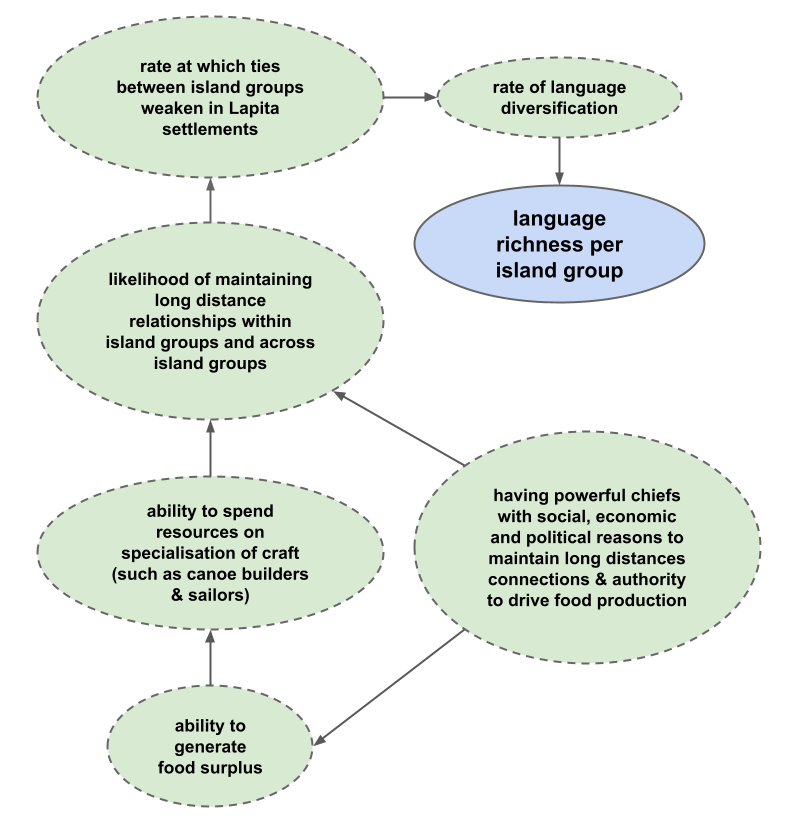
\includegraphics[width=\textwidth]{Predicting_lgs_DAG_andy.png}
\caption{Directed Acyclic Graph of the argument presented in \cite{pawley2007}. Blue = variable to be predicted (response).}
\label{Predicting_lgs_DAG_andy}
\end{figure}

Fig. \ref{Predicting_lgs_DAG_full} in \ref{appendix_DAG_def} contains a larger version that incorporates more of the suggested linkages beyond those suggested by Pawley, for example, that political complexity may affect the modularity and interconnectedness of social networks and this, in turn, affects language splitting. However, most of these factors are more difficult to measure or have not been measured (dashed outlines in the DAGs), whereas ``political complexity'' is a variable in the Ethnographic Atlas (c.f. \citet{gray1998ethnographic}).

In a similar vein to Pawley, \citet{curriemace2009} suggests that more stratified societies are correlated with larger language areas in Africa and Eurasia. If one language covers a large area, then the number of languages per square kilometre is lower than otherwise --- the language density is lower. Their research can be interpreted to mean that more stratified societal structures are more capable of sustaining linguistic homogeneity over a larger geographical area (or possibly reducing diversity by cultural dominance and warfare). Greater maintenance of cultural homogeneity would result in less language splitting over larger areas, and therefore a larger language area correlates with greater stratification. The approach is different from \citet{pawley81, pawley2007}, but the scientific line of argumentation is similar.

Returning to language richness in Remote Oceania, a significant factor to consider besides those already discussed is contact --- in particular with people from the New Guinea region (c.f. \citet{ross2017_new_guinea_region}). Prior to European colonisation, all indigenous communities of Remote Oceania spoke the languages of the Austronesian family (see Fig \ref{RO_overnight_coloured_dots}). This family has its ultimate origins in Taiwan, and spread into the Remote Oceania approximately 3-4,000 years ago (c.f. Fig. \ref{austro_expansion_bellwood}). The peopling of New Guinea, the Bismarck archipelago and much of the Solomon Islands however is older than that, and there is a great amount of language and cultural diversity there that may have influenced Austronesian people during and/or after their journeys east. 

\begin{figure}[ht]
\centering
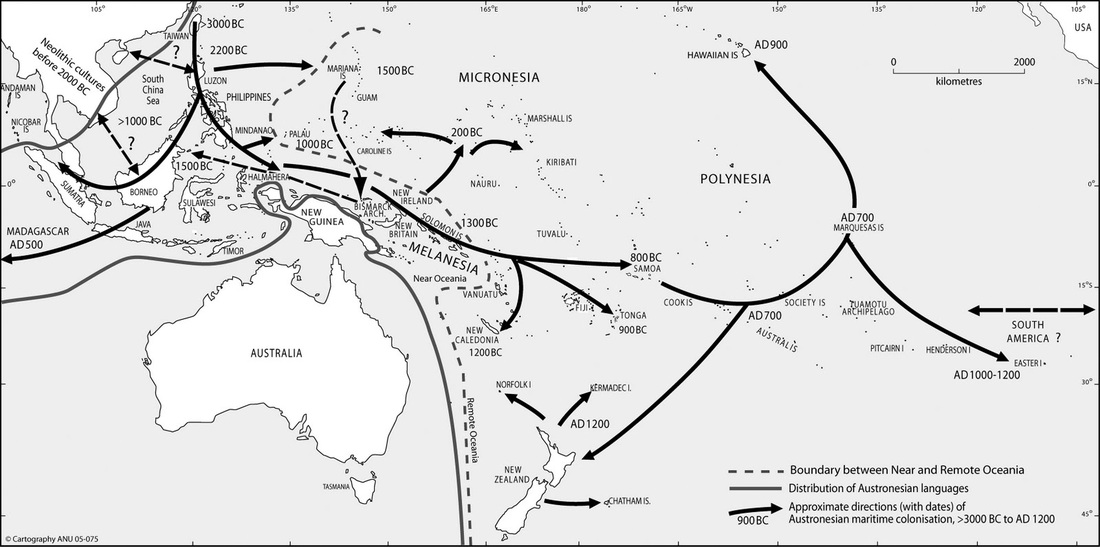
\includegraphics[width=15cm]{ANU_cartography.jpg}
\caption{Map of the expansion of the Austronesian language family, based on work by Peter Bellwood. Map made by ANU CartoGIS and Peter Bellwood.}
\label{austro_expansion_bellwood}
\end{figure}

Recent studies of ancient and modern DNA \citep{lipson_harvad_ancient_dna_vanuatu_2018, posth_jena_ancient_dna_vanuatu_2018} have shown that there is evidence of significant levels of genes that are associated with origins in non-Austronesian speaking communities from New Guinea and Solomons among Vanuatu people. The suggestion is that while the initial settlement of Remote Oceania was likely to be Austronesian (i.e. genetically similar to Asian populations), there have since been more people coming who have non-Austronesian ancestry from the New Guinea region. Interestingly, \citet{posth_jena_ancient_dna_vanuatu_2018} highlight that this had little effect on the languages of the region, communities still speak languages that are clearly Austronesian in origin.

Likewise, further studies such as \citet{liu2022ancient} show similar influence from New Guinea and Solomons northwards in Palau, Chuuk and Pohnpei island groups. It is becoming increasingly clear in the overall scientific literature on the ancient history of Oceania that there were a lot more connections and interactions than previously postulated --- including to island groups of Near Oceania. It is not the case that people travelled to one place, and then stayed put there with little influence from other people of Oceania. Oceania is an interconnected place today, and it was historically too.

It is possible that these interactions, which were more frequent in Vanuatu than in Polynesia, have implications for many domains of human life --- including political organisation and language diversity. Linguist and anthropologist \citet[104]{lynch1981melanesian} has stressed the relevance of contact with non-Austronesian communities from New Guinea, Bismarck, Bougainville and the Solomon Islands as a key factor in explaining why there are more languages in Vanuatu compared to the rest of Oceania \footnote{\citet{lynch1981melanesian} uses the terms ``Papuan'' and contrasts Melanesia and Polynesia. I have chosen to summarise him here in more precise terms in relation to how his work impacts the current study. He writes specifically about the influence of languages of New Britain, Bougainville, central Solomon Islands, Manus and the southeast of New Guinea mainland (Oro province, Milne Bay province and National Capital District) on Oceanic languages of those regions and in Temotu.}. Lynch does not offer a precise account but outlines several different potential scenarios whereby contact with non-Austronesian groups caused greater diversification among Oceanic languages.

Unfortunately, it is difficult to incorporate data on contact with non-Austronesian speakers explicitly in the models of this study. This is primarily due to lack of information on this variable in island groups such as Kanaky (New Caledonia), Ratak \& Ralik (Marshall Islands), Marquesas, Aotearoa and other island groups. However, this factor is very important and we will return to it in the discussions.

%could have impacted the differences in language diversification rates that we see in the region. However, unfortunately, there is not enough data for this to be included as a factor in the analysis of this study but it may be approximated by proxy-variables such as time depth of settlement


%\emph{\textcolor{red}{(Note to Andy, Simon, Mark and Nick: it is possible to include Papuan contact as a rather granular variable in the analysis. I have tried running a variable that just classifies each island group as "Melanesian" or "Not Melanesian" for example. That variable did not come out as significantly predicting the language diversity. It also felt a bit too crude. I talked to Beth about it and she recommended me to leave it out. However, if you would like I can keep it in and give caveats. I don't know yet of any DNA study that I can use for this. Both Posth et al and Lipson et al don't sample New Caledonia or Fiji at all, which makes it tricky to use here.)}}

%\footnote{Note that this is separate from theories of effects of culture and environment on the \emph{nature} of language, such as the work by \citet{wraygrace2007}, \citet{lupyandale2010} and \citet{raviv2019compositional}. Their work focusses on why different kinds of interactional patterns has consequences for the compositionality/complexity of a language. For this study, we are concentrating on linguistic \emph{diversity} as opposed to \emph{disparity}.}.

Finally, there has been a growing interest in environmental effects on language diversification\footnote{For a longer summary of recent studies of language diversification, see \citet{gavin2013toward} and \citet{greenhill2015demographic}.}. One of the oldest and most influential bodies of work in this vein is by Nettle. \citet{NETTLE1998} showed that there is a correlation between number of languages per country and ecological risk (as measured by mean growing season). Nettle suggests that high-risk environments encourage wider social networks and therefore reduce the number of languages in that area. \citet{hua2019ecological} expanded on this idea and explains that ``Smaller social groups are presumed to be more likely to be stable and self-sufficient in areas with a more abundant and reliable year-round food supply.'' \citet{hua2019ecological} constructed a more complex and fine-grained model of how environmental factors influence language diversity. They found that factors associated with risk (precipitation and temperature seasonality and season length) did indeed predict much of the distribution of languages in the world. Similarly, \citet{gavin2017process} showed that a simple model that takes into account rainfall and an upper bound of population size can to a large extent predict the distribution of indigenous languages in Australia. Given the success of these models, the amount and seasonality of rainfall and temperature variables are also included in our model predicting language diversity in Remote Oceania. 


%There are many more papers on demographic, cultural and environmental factors on language diversification, unfortunately there is not space enough here to relate them all. There are two overview papers that summarises many other studies on the topic very well --- \citet{gavin2013toward} and \citet{greenhill2015demographic}. I will refrain from copying their clear and instructive summaries and meta-analysis and instead direct the curious reader to seek those two papers out themselves should they want to explore the topic further.

In their study of global environmental predictors of language diversification, \citet{hua2019ecological} noted that there were certain areas that remained unexplained (New Guinea, Himalayas, West Africa and Mesoamerica). This may be an indication that the model needs to be adjusted to account for more variables or that the variables do not have the same effect globally. A recent study of language diversification in North America \citep{Pacheco_Coelho_2019} showed that the best predictors of language change may vary from place to place and that the factors are interlinked causally in a complex manner. Their study included environmental variables and data on the population. The authors note that political complexity might be an important variable too, but they were, unfortunately, unable to include it \citep[7]{Pacheco_Coelho_2019}.

This study focuses on a particular hypothesis concerning a particular region of the world. It is possible that these models perform less well globally and the results should primarily be compared against the specific theories of \citet{lynch1981melanesian} and \citet{pawley81, pawley2007} about Remote Oceania. As one of the few studies to include data on both environmental and socio-cultural variables, it is able to contribute a valuable perspective to the field of language diversity mechanics.

\FloatBarrier

%The cultural variables in this study are taken from D-PLACE \citep{d_place_all}, environmental data from ecoClimate \citep{ecoclimate} and archealogical dates from \citet{rieth_cochrane_2018}. The cultural variable of ``political complexity'' has been complemented with datasets from \citet{sheehan2018coevolution} and ethnographic sources. The archaeological dates were also further supplemented with data from \citet{levin_seikel_miles_2019, pol_outliers_stat_art, intoh2008ongoing, intoh2007reconnaissance} and \citet{Napolitano_et_al_yap}. 


%We will also be using two environmental variables taken from D-PLACE: Net Primary Production (NPP) and NPP predictability. The Net Primary Production is the grams of carbon uptake per square meter of land per month.
\FloatBarrier
\section{Materials and Method}
\label{pol_complex_method}
The approach of this paper is to gather relevant data on island groups and their societies and then fit a statistical model which aims to predict the number of languages given all the variables. From the composition of variables in the resulting model we can infer which have the greatest predicting power when they are co-estimated.

The unit of analysis is ``island group''. We cannot use modern political boundaries (``French Polynesia'', ``Cook Islands'' etc) because they are often historically and culturally inappropriate. As we want to capture something about the communities at large we are not satisfied with using individual islands. For these reasons, we use two different ways of grouping islands: overnight sailing distances and shared language (see appendix \ref{sec:island_geo} for details).

%Predicting_lgs_DAG_full

A simple test of Spearman's Rank Order correlation reveals that the number of languages and political complexity per island group are indeed moderately correlated (rho  = -0.4, \emph{p} value < 0.001 for islands grouped for shared language). However, this is not sufficient. We want to investigate whether this correlation still holds once we explicitly incorporate other variables that we expect might explain language diversity as well, such as time-depth and environmental factors. 

Variables were included in the model if they meet all three of the following criteria: a) have been suggested as relevant in previous literature, b) there is enough data on the variable in a published source and c) if they relate to the response variable (language richness) in a non-mediated manner (c.f. \citet{pearl1995causal}). This results in the following variables:

\begin{itemize}
\item \textbf{response variable}:
\begin{itemize}
\item language classification, based on \citet{glottolog40} and other sources (see Appendix \ref{sec:language_class}).
\end{itemize}
\item \textbf{predicting variables:}
\begin{itemize}
\item number of vertical levels of jurisdictional hierarchy per society \footnote{Nota Bene that there are other kinds of political complexity besides vertical, for example, horizontal complex exchange networks. See Appendix \ref{appendix_def_pol_complex} for more.}, based on the Ethnographic Atlas \citep{gray1998ethnographic, d_place_all}, \citet{sheehan2018coevolution} and own modifications. Also known as ``political complexity'' and ``EA033'' (see appendix \ref{appendix_def_pol_complex} for details on definition and coding).
\item archaeological dates, grouped into waves \citep{intoh2007reconnaissance, intoh2008ongoing, rieth_cochrane_2018, levin_seikel_miles_2019, pol_outliers_stat_art, Napolitano_et_al_yap}. (See appendix \ref{appendix_def_dates} for details.)
\item historical environmental data from \citet{ecoclimate}: mean temperature, temperature seasonality, mean rainfall and rainfall seasonality. (See appendix \ref{appendix_environ} for details.)
\item environmental data from NASA satellites \citep{running2021modis_aqua, running2021modis_terra}: Net Primary Productivity. See appendix \ref{appendix_environ} for details.)
\item island geography (latitude and shoreline) from the Global Self-consistent, Hierarchical, High-resolution Geography Database (GSHHG) \citep{wessel1996global}.  (See appendix \ref{appendix_environ} for details.)
\end{itemize}
\end{itemize}

The variables Net Primary Production (NPP; the amount of biomass or carbon produced), temperature \& rainfall (mean and seasonality) and absolute latitude are all associated with the suitability of a place for life and they correlate with each other, at least to some degree (c.f. Figs \ref{SPLOM_medium_all_variables} and \ref{SPLOM_SBZR_all_variables}). In this study, they are all tracking a similar concept: the suitability for human populations to thrive in smaller groups. Because of this, we are running a Principal Components Analysis on all seven variables, this allows us to extract a variable that explains most of the information. We ran a Non-Graphical Cattel's Scree Test \citep{cattell1966scree, R-nFactors} to determine the number of optimal components (overnight sailing distance island groups = 2 PCs, shared language island groups = 3 PCs). For more details, see Appendix \ref{appendix_eniron_PCA}.

In order to create a formula for the statistical model, we consider the suggested causal relationships based on previous research (see section \ref{sec:previous_research}). Besides the effect of the environmental variables on language richness, we also hypothesise that there can be a joint effect with the size of the island. Similarly, the time-depth and size of islands may also interact. 

The relationship between variables can be represented in a formalised manner in a Directed Acyclic Graph (DAG; \citet{pearl1995causal} and \citet{mcelreath2020statistical}), see Fig. \ref{Predicting_lgs_DAG_slimmed}. For the full DAG, including excluded variables and variables with missing data, see appendix \ref{appendix_DAG_def}. Interactions are denoted with a deterministic node labelled with $\ast$. 

\begin{figure}[!ht]
\centering
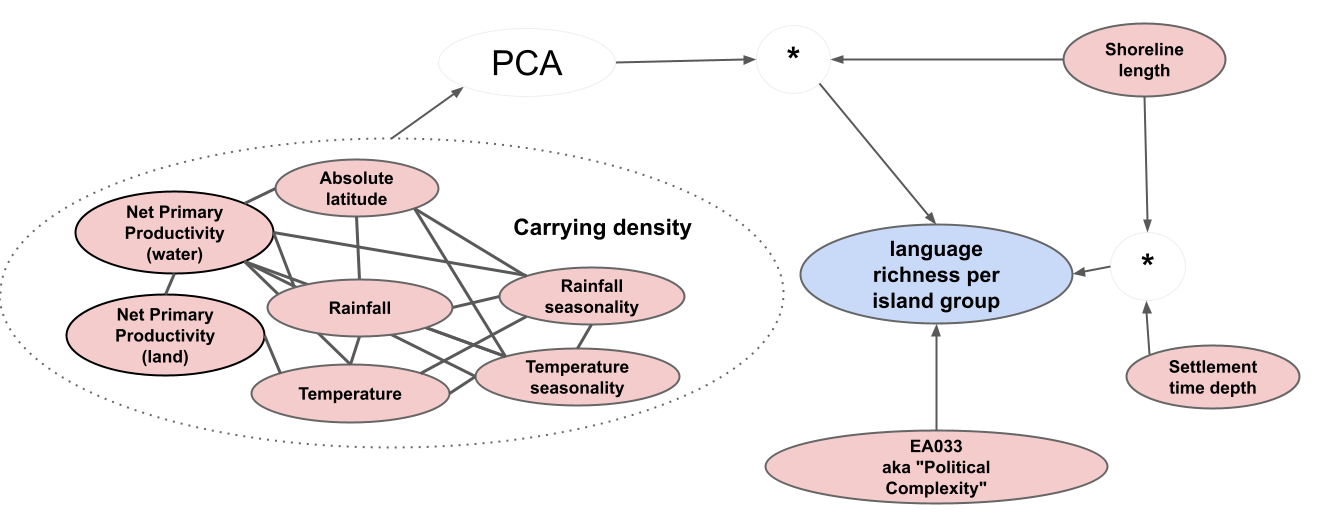
\includegraphics[width=16cm]{Predicting_lgs_DAG_slimmed.png}
\caption{Directed Acyclic Graph of the variables in this study (DAG, c.f. \cite{mcelreath2020statistical}). Blue = variable to be predicted (response), red = predictors. Asterisk nodes represent variable interactions, a type of deterministic DAG-node. PCA represents Principal Components Analysis. PCA was run on the incoming variables, and the optimal number of components (given a Non-Graphical Cattel's Scree Test) were carried forward. Terra and Aqua are the names of the NASA satellites.}
\label{Predicting_lgs_DAG_slimmed}
\end{figure}

This results in the following model formula\footnote {Settlement order was reversed from Fig. \ref{dates_map} such that high numbers represent further back in time.}:

\begin{quotation}

\texttt{Number of languages \textasciitilde{} Political complexity (mode)} + \\
\indent \indent \texttt{Environmental PC1  *  Shoreline (log10 +} \\
\indent \indent\texttt{Environmental PC2  *  Shoreline (log10 +} \\
\indent \indent (\texttt{Environmental PC3 *  Shoreline (log10) +} \\
\indent \indent\texttt{Settlement order *  Shoreline (log10)} \\
\end{quotation}

Shoreline was log-10-transformed. All predicting variables were then also normalized in the conventional manner by subtracting the mean and dividing by the standard deviation.

To test the impact of several variables predicting the same response variable we can use a Bayesian Regression Model \citep{gelman2006data, burkner2017brms}. The distribution of languages per island group is over-dispersed. There are many island groups with one language and only a few with higher numbers (see Figs. \ref{polygon_plot_SBZR} and \ref{polygon_plot_medium} in Appendix \ref{sec:island_geo}). For the overnight-sailing island groups, the group that contains Vanuatu and Temotu has 130 languages, whereas most island groups in Polynesia have 1 or 2. This skewed distribution necessitates a Poisson distribution for the response variable in the model, which is able to adjust the relationship between the mean and the variance appropriately\footnote{This issue was also faced by \citet{gavin2012island} in their study of environmental factors in language diversification in the Pacific. They chose another approach, a reciprocal transformation, based on model fitness compared to two other kinds of transformations of the response variable.}. For further details on the model set-up, see appendix \ref{appendix_model_settings}.

Due to missing data, we are testing our models over 65 out of 104 shared language groups and 56 out of 67 overnight distance groups. This sample still contains some of our more extreme sites, like Santo, Kanaky (New Caledonia mainland) and Malakula. Variables that did not cover Vanuatu and New Caledonia with enough specific data-points are not included in this study, for example historic population data, non-Austronesian gene flow or jurisdictional hierarchy within local communities. 

The results were calculated in R 3.6.0 \citep{R} using the function \texttt{brms::brm()} \citep{burkner2017brms}, tidyverse suite \citep{tidyverse13} and the modEvA-package \citep{barbosa2016package}. For a full list of packages used, see appendix \ref{appendix_r_packages}.

\FloatBarrier
\section{Results}
% BARG
We will first go through the outcomes for the shared language island groups, and secondly the overnight distance groups. In common for both is that political complexity is a relevant predicting factor, with a negative effect (the more political vertical levels, the lower the number of languages). This lends support to the proposal by \citet{pawley81} and \citet{pawley2007}. However, there are details of the result that suggest that the effect may be due to non-Austronesian contact rather than political complexity \emph{per se}.

Fig.~\ref{medium_model_predict} shows the actual observed language counts (purple triangles) and predictions of this model (green boxplots). The model does predict that Santo, Kanaky and Malakula have the highest language counts in the dataset. Our observed language counts for Santo, Kanky and Malakula are 24, 29 and 33 respectively. The model is very close for Santo and Kanaky for its average prediction value but underestimates Malakula by 17 languages. The absolute average difference between the mean predicted values and the observed is 2.8.

%The results show that the model run with the shared-language island groups have an absolute average of difference between the predicting number of languages and observed of 2,8 the overnight-sailing distances island groups of 4.3 Fig.~\ref{medium_model_predict} and Fig.~\ref{SBZR_model_predict} illustrate the specific predictions the models make compared to the observed language counts. 

\begin{figure}[ht]
\centering
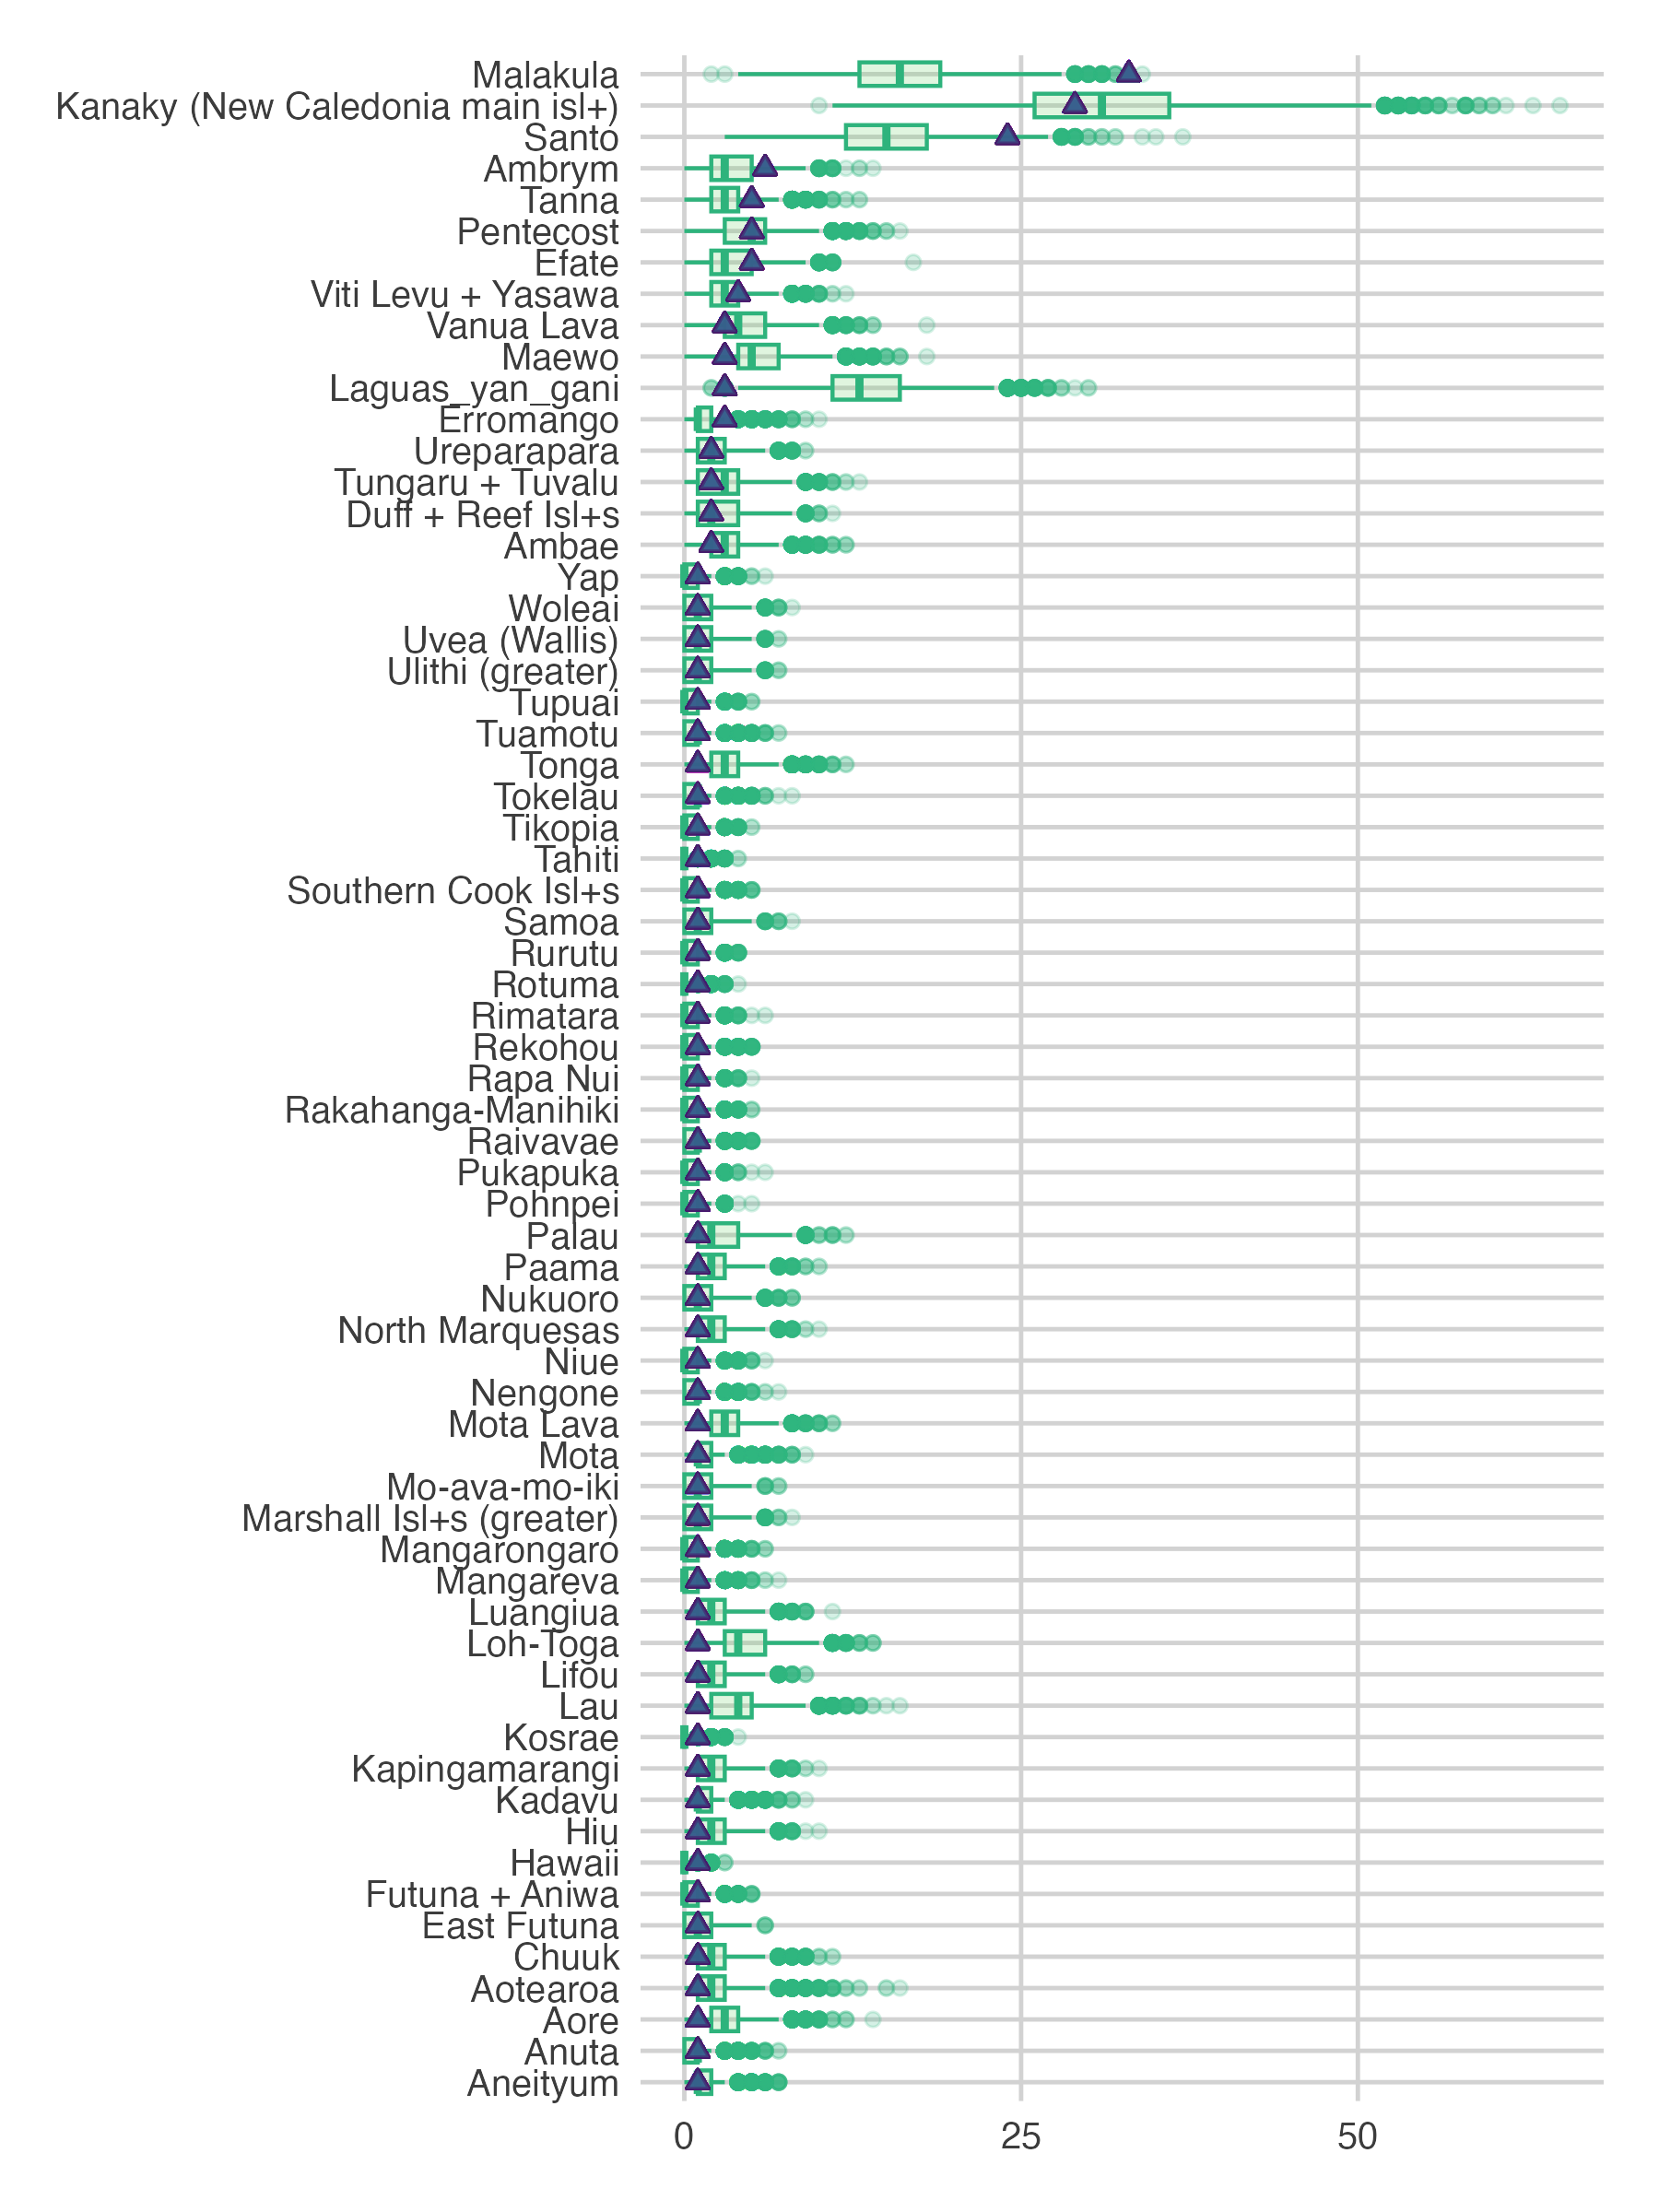
\includegraphics[width=0.75\textwidth]{brms_predict_medium.png}
\caption{Prediction from the model with island grouped for shared language. Number of languages is on the x-axis, observations on the Y. The dark blue triangles represent the observed number of languages, the green boxplot the predictions of the model. Average absolute difference between the mean of the predictions and the observed = 2.8.}
\label{medium_model_predict}
\end{figure}

For the shared language island groups, political complexity (EA033) is the only variable that is different from zero, i.e. the full coefficient distribution does not overlap zero. If we only consider the 95\% credibility interval, as is common practice in statistics, there is one additional term that does not overlap zero: shoreline in interaction with time-depth. Fig \ref{brms_SBZR_group_full_effect_ridge_panels} in Appendix \ref{appendix_supp_figs} shows the full distributions.

If we drop one island group out at a time and re-run the model, we can asses which island groups represent the largest challenge to fitting the model. Most of the island groups can be removed with little effect (see Fig. \ref{brms_medium_dropped_out_plot_diff} in \ref{appendix_supp_figs}), however, when Malakula (central Vanuatu), Kanaky (New Caledonia main island) and Santo (central Vanuatu) are left out, the difference becomes much lower. They are the three island groups with the highest number of languages (see Fig \ref{polygon_plot_medium} in appendix \ref{sec:island_geo}). Political complexity remains the most important predicting factor in these three models, the coefficient distributions do not overlap with zero.

%and shoreline in interaction with time depth are the variables that have a significant impact, i.e. do not cross zero (see coefficent distributions in Figs.  and \ref{brms_medium_group_full_effect_ridge_panels} in appendix \ref{appendix_supp_figs}).

For the overnight-sailing distances, several island groups are much larger than the previous grouping. The islands of Vanuatu  (including Anuta and Tikopia) and Temotu are all within the same group (see Fig \ref{polygon_plot_SBZR} in appendix \ref{sec:island_geo}; this is similar to the groups considered in \citet{pawley2007}). This also leads to a larger discrepancy between the number of languages, with Vanuatu and Temotu having 130 and S\={a}moa still only one. The average absolute difference between the predicted and observed number of languages is greater than for the previous grouping --- 4.3. Fig \ref{SBZR_model_predict} shows the prediction vs observed per island group.

\begin{figure}[ht]
\centering
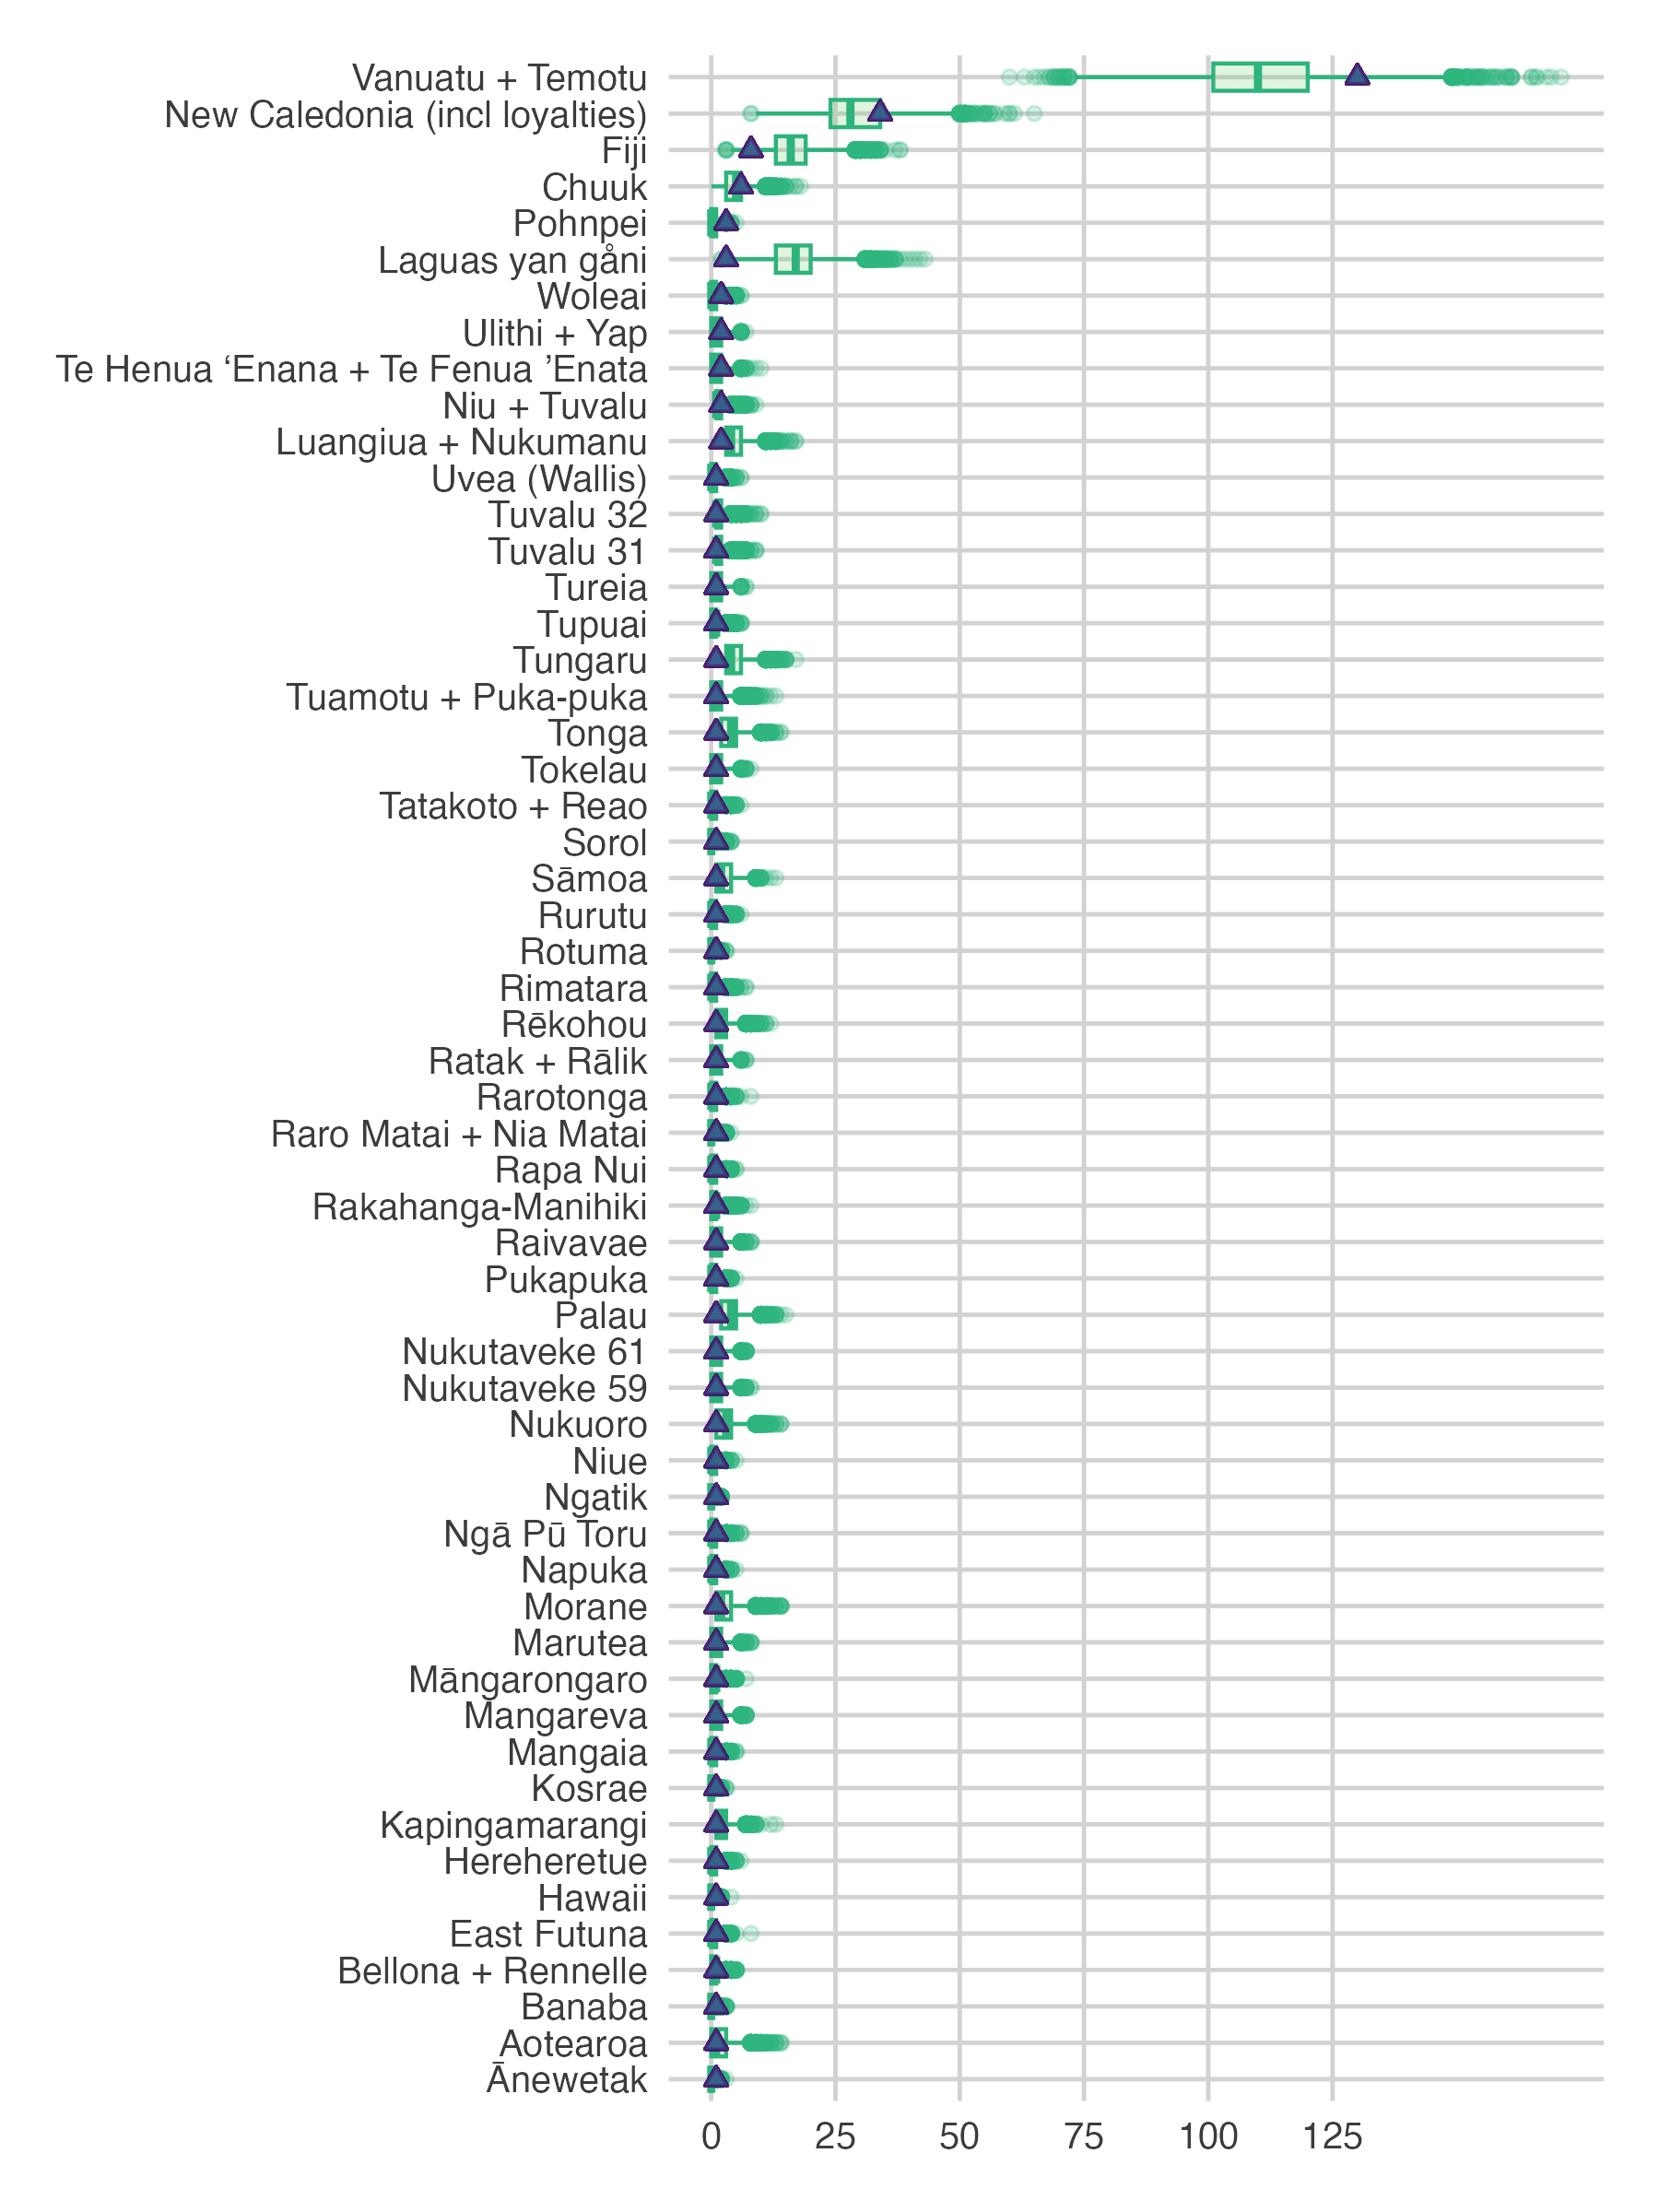
\includegraphics[width=0.75\textwidth]{latex/brms_predict_SBZR.png}
\caption{Prediction from the model with island grouped for overnight sailing distances. Number of languages is on the x-axis, observations on the Y. The dark blue triangles represent the observed number of languages, the green boxplot the predictions of the model. Average absolute difference between the mean of the predictions and the observed  4.3.}
\label{SBZR_model_predict}
\end{figure}

The most important variables in this model (i.e. coefficient distribution does not overlap 0) were: shoreline, political complexity, time depth and time-depth in interaction with shoreline (see Fig \ref{brms_SBZR_group_full_effect_ridge_panels}). However, if we drop out Vanuatu + Temotu this no longer holds. When Vanuatu + Temotu are left out, the coefficient distribution of political complexity overlaps zero. Instead, the environmental PCs, Shoreline and time depth are relevant predictors.\footnote{They are relevant if we consider the 95\% credibility interval. If we take the full distribution, all terms overlap zero.} When Vanuatu + Temotu are dropped out, the overall difference between predicted and observed values goes down significantly (from 4.3 to 2, see Fig. \ref{brms_SBZR_dropped_out_plot_diff}). If we ask this model that has been trained without the Vanuatu + Temotu data to predict how many languages are there, it grossly underestimates and proposes 7 languages (observed = 130). If we drop out any other island group (including Kanaky), political complexity remains a significant factor as it does in the model with all observations.

For tables of the effect Estimate, Rhat and ESS for both models, please see Appendix \ref{BRMS_model_tables}.


%Most of the island groups in this dataset have only one language, and this seems to have caused some issues (despite the Negative Binomial distribution). The model does best at predicting languages in Polynesia (which is dominated by island groups with only one language). Islands groups in Polynesia can have a very long coastline (like the Paumotu archipelago of French Polynesia) or very short one (like Niue). There is not as much difference in shorelines between islands of Vanuatu. The model seems to have struggled with using shoreline to predict languages globally, even leading to the result that Shoreline as a standalone term comes out in the model as negatively predicting the number of languages (though not with a \emph{p} value that passes traditional thresholds of significance). 

%Among the island groups the model predicted \textit{least} successfully is Paama, a very small island of Vanuatu with one language. The model predicted 5.2 languages, the observer value is one. 

%Paama is coded 1 for political complexity \citep{bonnemaison1996graded} and as part of the third wave of settlement \citep{rieth_cochrane_2018}. Most island groups that are coded as low for political complexity and low for settlement are found in Vanuatu and can be somewhat differentiated by Shoreline with Malakula and Santo having longer shorelines and more languages. However, in the full sample there are island groups with much longer shorelines and only one language (Aotearoa and Paumotu). The estimates of the model show that while the interaction of Shoreline and Settlement order has a significant positive influence as an interaction, the effect is not large.



%brms_SBZR_dropped_out_plot_diff


\FloatBarrier
\section{Discussion}
\label{pol_study_discisson}
The results indicate that political complexity could be relevant for understanding the dynamics of language diversification in Remote Oceania, but further studies are needed --- especially regarding Vanuatu. 

When the island group Vanuatu + Temotu was dropped, the model for overnight sailing island groups no longer drew on political complexity as a relevant predictor of language richness. This may indicate that it primarily made use of the term to tell apart Vanuatu + Temotu from all other island groups. Vanuatu + Temotu is by far the island group with the most languages, 130, and it is dominated by societies that are classed as level 1 on the scale of vertical political complexity used by the Ethnographic Atlas \citep{gray1998ethnographic} and other studies \citep{watts_2018}, see Fig. \ref{pol_complex_map} in appendix \ref{appendix_pol_complex}).

Furthermore, if we tease apart the argument concerning political complexity (for example in the full DAG in Fig. \ref{Predicting_lgs_DAG_full} in appendix \ref{appendix_DAG_def} or Fig. \ref{Predicting_lgs_DAG_andy} in section \ref{sec:previous_research}), we find that conceptually the link between the number of languages and political complexity is not direct. It could be mediated through other factors such as network modularity, the propensity to maintain long-distance contact etc. 

\citet{watts_2018} found that politically complex societies in Oceania became Christian at a faster speed. This may indicate that changes propagate through a population quicker if the society is not egalitarian. If Christianity spreads faster in societies with higher complexity, it is possible to reason that other changes also might spread faster. If changes propagate quickly throughout a population, that leaves less possibility for diversification through natural drift or groups in the periphery staying more archaic compared to the centre. This interpretation relies on the understanding that the variable for political complexity (EA033) reveals something not only about jurisdictional power relationships in a given society, but also captures something about the social network of \emph{all} of its members (not just the leaders). Under this theory, people living in societies with higher political complexity would be able to travel further and have wider-ranging social networks, which in turn would lead to greater internal cultural homogeneity.

Maintaining long-distance contact can indeed be a function of shared cultural identity. \citet[218-291]{skirgaard2020multilevel} notes that there are not only fewer languages in the island groups of Polynesia, but they are also more similar to each other lexically than languages in Vanuatu are. This relationship does not hold for grammatical features however, languages in Polynesia are similarly different from each other grammatically as languages of Vanuatu and other island groups in Remote Oceania are (as measured by Grambank features, \citep{grambank_release}). It has been suggested, by \citet{silverstein1981limits}, \citet{francois2011} and others (c.f. \citet{mansfield2023dialect}), that communities pay special attention to words and sound differences as emblematic of shared ties --- but grammar tends to fly under the radar in this respect. This difference between Vanuatu and Polynesia in terms of lexical dissimilarity and language richness, but the similarity in terms of grammatical diversification may indicate that the cause does indeed lie in attitudes and social network organisation rather than merely time and environmental factors.

\citet{curriemace2009} argue that the reason behind their results (higher political complexity = larger language areas) is that societies with higher political complexity are more likely to be able to replace existing groups in an area, or otherwise incorporate (and possibly assimilate) them. It may also be the case that diversity in Polynesia was reduced by later expansionist efforts by societies with higher political complexity. For example, the island of Niuafo'ou which lies between Tonga, 'Uvea and S\={a}moa is home to a language that is most closely related to 'Uvean. This language has however become \emph{more} similar to Tongan during the period of Tongan domination in the area 1000-1300's (see \citet{aswani1998tongan} and \citep[2-9]{tuskamoto_niuafoou}). It may be that politically complex societies do not only \emph{maintain} homogeneity by continuing being in contact after first settlement, but can also reduce diversity which emerges after settlement through incorporation and cultural dominance later.

Whatever the political complexity variable is tracking, it is clear that it is one of the variables that most clearly picks out Vanuatu and Vanuatu is the place with the most languages. Where did this difference in societal organisation come from? As previous studies have indicated (e.g. \citet{lynch1981melanesian}), the answer may lie in contact with people from New Guinea and Solomons. It is possible that contact with non-Austronesian speaking communities further west brought with it societal changes to Vanuatu and some other islands that had made history go a different way there than in islands further east. Besides the possible cultural influence on attitudes and societal organisation, they may also have brought with them their own cultural heritage which would add to the diversity in itself.

%In order to understand language diversification, we need to understand the steps of the process. Before languages have split into different mutually unintelligible varieties, 

%The \citet{WLH1968}



%Both models include political complexity as a statistically significant factor for predicting language diversity in Remote Oceania which gives support to the hypothesis tested in this study. As expected, space and time also came out as significant factors. This indicates that the longer time people lived in a place and the longer shoreline/more land there was, the more languages arise. This is in line with previous research. \citet{curriemace2009} found that politically complex societies (``ethnolinguistic groups'') cover a larger geographical area than societies with low political complexity.  Assuming one language per society\footnote{By using language area as a measurement of the size of ethnolinguistic groups/societies, \citet{curriemace2009} make this assumption.}, a random 10 km$^2$ sample which has a high average value for political complexity (averaging over all language polygons that are found in the cell) will then have fewer languages. For example, the language Turkish is associated with a political complexity score of four \citep{d_place_all} and covers a large area whereas the many languages of the nearby Caucasus are generally coded as low political complexity and cover smaller areas \citep{ethnologue2005}. If we take a 10 km$^2$ sample in Anatolia (where Turkish is spoken) we find fewer languages and higher complexity on average than if we sample the same sized area in the Caucasus. Similarly, we find fewer languages per island group in Remote Oceania the higher the average political complexity.

%A counterexample to this trend globally is the presence of large areas covered by language societies with low political complexity and majority pastoralist subsistence strategies. \citet{curriemace2009} found such cases, but their results concluded that the best predictor for the overall global patterns in their data was still political complexity. Another possible counterexample might be regions of many societies with high complexity where each society covers a small area in close proximity to each other. This is arguably the case for historic city states in Ancient Greece as these covered fairly small areas and had many political levels (see \citet{cartwright_2013}, and \citet[19]{sealey1976history}). However, the city states of Ancient Greece are usually all described as speaking different dialects of the same language, not different languages. This means that the language area of Ancient Greek (which is what \citet{curriemace2009} measured) would still be large and the average political complexity high, which would support their hypothesis.



%It is beyond the scope of this study to fully investigate the causality of language diversification in Remote Oceania. Causality in cultural evolution is very complicated, since factors can interact on many levels and it is difficult to control for unknown variables and proxy effects (c.f \citet{roberts2013linguistic}). In this instance, we will be satisfied with testing if there is a correlation between societal structure and language diversity that is still signifncant once environmental and settlement time has been incorporated into the model.

Unlike the studies by \citet{gavin2012island}, \citet{hua2019ecological} and others, the results of this study indicate that environmental factors such as rainfall seasonality and isolation have less of an impact on language diversity in Remote Oceania. This is most likely because most of the island groups share a similar climate, and there is therefore not enough variation to tease them apart.

%As can be seen from the specific predictions the models make (Fig. \ref{medium_model_predict} and Fig. \ref{SBZR_model_predict}), neither model accurately predicts the key island groups in our dataset (Vanuatu, Kanaky (New Caledonia) and Temotu). Explaining the difference between Melanesian Remote Oceania and the rest is the most important factor in evaluating our hypothesis. Therefore the results should be interpreted as ultimately inconclusive. 

%\citet{Pacheco_Coelho_2019} explore an approach where the predictive power of each variable is not fixed, but changes with respect to location. Such an approach may give more insight into this dataset, and is left as future work.

%Possible limitations with this study are: a) the way that islands groups are defined, b) the manner in which the over-dispersion was accounted for and c) poor measurements of, or missing, key variables. Concerning (a), it may be that a grid-approach (c.f \citet{hua2019ecological}) is more appropriate. One of the problems with a grid approach is that it may work less well in an oceanic environment where connections between islands are not accounted for appropriately, but it should be tested in a similar manner to this study to evaluate if this indeed is a problem. A more finer grained approach similar to  \citet{gavin2012island} where each landmass is the unit of analysis may also be interesting. Both of these approaches may also aid with (b). There are other ways of accounting for (b), over-dispersion in data, besides a Negative Binomial distribution. For example, \citet[4-5]{gavin2012island} used the reciprocal of the language count. Regarding (c), \citet[4-5]{gavin2012island} found that Isolation was a significant variable in their models for predicting language diversity on Oceania (including Near Oceania). It is possible that the manner in which isolation was calculated here was suboptimal and that one or several of the other measurements of Isolation is more appropriate (see section \ref{sec:island_geo}). It was also not possible to include measurements of non-Austronesian contact in this study due to poor data coverage despite the fact that it could be a relevant factor (c.f. \citet{lipson_harvad_ancient_dna_vanuatu_2018, posth_jena_ancient_dna_vanuatu_2018}). 
 

\FloatBarrier
\section{Conclusions}
This study investigated the hypothesis that besides time depth and environmental factors (c.f. \citet{curriemace2009, gavin2012island, hua2019ecological} and \citet{Pacheco_Coelho_2019}), language richness in Remote Oceania is also significantly influenced by interaction patterns that can be measured by political complexity (c.f. \citet{pawley81, pawley2007}). The results lend support to this thesis, with some caveats. 

Political complexity is, perhaps unsurprisingly, a complex variable. There are a number of phenomena in our social world that it could track, including network dynamics and in the case of Remote Oceania specifically --- contact with communities in New Guinea and Solomon Islands. It is clear that in terms of constructing predictive models, it contributes significant power to the case of island groups in Remote Oceania and language richness. However, in order to understand the situation we need to deconstruct this concept further and conduct studies that tease apart the specific circumstances --- especially in Vanuatu. 



%The results of this study lend support to the theory that political complexity is a significant factor in predicting language diversity in Remote Oceania beyond what can be accounted for by environmental factors, size of islands and time-depth of human settlement. However, 


%Due to failed predictions for key regions (Vanuatu in particular), and other methodological limitations, this hypothesis needs to be investigated in future research. It appears that there is still much left to understand about language diversification in the region, and in Vanuatu in particular.

%Future studies should use a grid and/or otherwise more fine grained approach to sampling, test different statistical methods that deal with over-dispersed data, and attempt to include better data on isolation, population and non-Austronesian contact. This study concentrated on the number of languages in a place, but it may also be revealing to include measurements of how different the languages are from each other, in lexicon and/or structure.


%Linking study 2 to study 3
%In study 2 we show that yes internal structure of a community is a factor, that means that the variation within a community can be linked to overall change between communities. In the next study we will look into more detail the way that linguists have approached these two levels of variation, micro and macro.


\newpage



\newpage
\singlespacing
\bibliographystyle{unified_edit_HS_SFM}
\bibliography{latex/HS_Oceanic, latex/used_pkgs, latex/pol_complex_refs}
%\singlespacing



\newpage
\section*{Acknowledgements}

The research leading to this paper has received funding from the Department of Linguistic and Cultural Evolution, Max Planck Institute for Evolutionary, the School of Culture, History and Language at the Australian National University and from the Australian Research Council through The Wellsprings of Linguistic Diversity Laureate Project (awarded to Professor Nicholas Evans 2014-2018) and the Centre of Excellence for the Dynamics of Language (CoEDL).

I am fortunate enough to have colleagues in academia who have been generous enough to discuss conceptual methodological matters with me, these are Stephen Mann, Angela Chira, Russell Gray, Oleg Sobchuk, Richard McElreath, Tiago Tresoldi, Michael Dunn, Hannah Haynie, Outi Vesakoski, Fredric Blum and Luke Maurits. I am also grateful for the advice of Mary Walworth, Ray Harlow, Andrew Pawley, Paul Geraghty and Alexandre François concerning language classification; Matthew Spriggs, Geoff Kushnick and Christopher Ballard regarding archaeology and anthropology of Oceania and finally Oliver Sheehan for helpful discussions regarding coding of the Ethnographic Atlas variables.

I also want to thank my PhD supervisors who reviewed earlier versions of this study for my thesis \citep{skirgaard2020multilevel} and provided insightful input; Nicholas Evans, Andrew Pawley, Mark Ellison and Simon Greenhill.

Any mistakes and misconceptions that remain are my own.

\newpage
\singlespacing
\appendix
\section*{Appendices}
\addcontentsline{toc}{section}{Appendices}
\renewcommand{\thesubsection}{\Alph{subsection}}

\subsection{Data and code availability}
\label{supp_data_availability}

All data in this study is available freely. The data has been gathered from multiple sources, and is aggregated and published along with the code for the study.

Global Self-consistent, Hierarchical, High-resolution Geography Database (GSHHG) \citep{wessel1996global}
the ecoClimate database \citep{ecoclimate} 
United States of America's National Aeronautics and Space Administration's Moderate Resolution Imaging Spectroradiometer (MODIS, \citet{running2021modis_terra, running2021modis_aqua}).

All the R-scripts for data wrangling, analysis and plotting are found on GitHub and Zenodo.

GitHub locations:
\begin{itemize}
\item predicting\_number\_lgs\_in\_remote\_oceania  \url{https://github.com/HedvigS/predicting_number_lgs_in_remote_oceania}
\item glottolog-cldf (v3) \url{https://github.com/glottolog/glottolog/tree/v3.0}
\item dplace-data (v) \url{}
%# double check versions
\end{itemize}

Zenodo locations:
\begin{itemize}
\item predicting\_number\_lgs\_in\_remote\_oceania  \textcolor{red}{TBA Zenodo-url}
\item glottolog-cldf (v3) \url{https://doi.org/10.5281/zenodo.437430}
\item dplace-data (v) \url{https://doi.org/10.5281/zenodo.5554395}
%# double check versions
\end{itemize}




\subsection{Data details}

\FloatBarrier
\subsubsection{Defining Remote Oceania}
The distinction of Near and Remote Oceania was first suggested by \citet{pawley1973dating}\footnote{This is the first occurrence of the two terms, although Green wrote earlier papers which included some of the ideas.} and was further elaborated on in \citet{green1991near}. This distinction is based on geology, flora and fauna. Near Oceania consists of chains of inter-visible large islands and archipelagos, whereas the islands and atolls of Remote Oceania are separated by much greater distances. 

There is a marked difference in the biodiversity of Near and Remote Oceania, due to the greater distances between islands in Remote Oceania. This has consequences for both flora and fauna, as \citet{green1991near} and \citet{pawley2007locatingoceanic} write:

\begin{quotation}
\noindent \emph{all terrestrial mammals other than rats and mice or those which accompanied people reach their eastward limit in the Solomons. The same applies to all fresh-water mussels, and most of the Palaeo-Oriental land-snail fauna. Thirty Papuan and Malayan genera of birds find their eastern limits here, as do 162 genera of seed-plants, about 24\% of the total.}
\end{quotation}
\begin{flushright} \citet[495]{green1991near}
\end{flushright}

\begin{quotation}
\noindent \emph{Even in marine life the difference is marked. The reefs of the Bismarck and Solomons show a much richer diversity of fish, molluscs, echinoderms, crustacea, seaweeds, and other edible life than those of Remote Oceanic [sic].}
\end{quotation}
\begin{flushright}  \citet[19]{pawley2007locatingoceanic} \end{flushright}

The greater distances between the islands of Remote Oceania is also the reason why they were settled by people much later than Near Oceania was (3,000 years versus 20,000-60,000 years ago). It was necessary to develop particular sailing techniques to traverse these greater distances in order to settle the region.

In this study, the region of Remote Oceania is defined slightly differently from the maps in \citet{green1991near} and \citet{pawley2007locatingoceanic}. All Northern Polynesian Outliers in Papua New Guinea and Solomons are incorporated, as is Mapia in northwest Papua New Guinea. The lines in the maps of \citet{green1991near} and \citet{pawley2007locatingoceanic} appear not to include these in Remote Oceania. I have included them in part to complete the Polynesian subgroup of languages and the languages of the Micronesian archipelagos, but also because it appears that these were not inhabited prior to the Austronesian expansion into the rest of Remote Oceania (c.f \citet[23]{kirch2012basline}) which suggests that they are sufficiently distant from the larger islands of Near Oceania to be counted as ``Remote''.

Regarding the terms ``Near'' and ``Remote'', there are two interpretations of what they are referring to:

\begin{enumerate}
    \item islands and atolls of ``Near Oceania'' are nearer \emph{to each other} 
    \item islands and atolls of ``Near Oceania'' are nearer to large landmasses west-wards, such as Australia.
\end{enumerate}

The difference between these two interpretations has no direct bearing on the study at hand, but the first one appears more fitting given the ecological framing of distance for people, flora and fauna to travel to colonise the new land. The islands of the Pacific are often construed as ``islands in a vast sea'' \citep{hauofa_1993} and a reading of ``Remote'' as ``far away from places of power/important places'' may enforce that understanding which is unnecessary and detrimental to our understanding of the history of the region (especially considering the importance of S\={a}moa and Tahiti as centres of power). 

\newpage
\FloatBarrier
\subsubsection{Defining ``language''}
\label{sec:language_class}
This study investigates factors influencing language diversification. The most central part of our data is the number of languages per island group; this is the response variable of our models. It is notoriously difficult to distinguish dialects, languages and language groups and there exist many different competing standards for defining languages. Linguists and others have debated these issues for a long time. Given their importance and centrality to this research, this section will give an introduction to the language identification standards adopted in two of the most commonly used resources: SIL International's ISO 639-3 codes for language names (which is implemented in Ethnologue \citep{ethnologue22}) and Glottolog's glottocodes.

It should be noted that while different language identification standards do differ, their findings do not vary dramatically. For example, SIL's Ethnologue states that there are 7,111 living languages today, Glottolog reports that there are 6,989\footnote{This the number of languoids in glottolog classifies as ``language'' and not labelled as ``extinct''.}. The difference between these two total counts is ``only'' 122 --- which is quite small considering how controversial language identification standards can be. This is in line with Nettle's observation that while linguists often disagree on how precisely to define a language, there is often considerable agreement in practice when it comes to categorising specific language varieties \citep[356]{NETTLE1998}.

The Summer Institute of Linguistics International (SIL) is the official Registration Authority of the International Organization for Standardisation (ISO) standard for codes to represent language names --- ISO 639-3. There are other ISO standards for languages, but ISO 639-3 is the most comprehensive and widely used. Most students and scholars are familiar with this code set from the SIL publication Ethnologue (which in 2016 became fully accessible only to paying subscribers, contributors and users from developing countries). However, it should be noted that the code set is also available independently of Ethnologue at https://iso639-3.sil.org/. The ISO 639-3 is technically separate from Ethnologue, and maintained by separate staff of SIL International.

The purpose of ISO 639-3 is to coordinate language names. There can be many different names for the same language, for example, Armenian is known both as ``Haieren'' and ``Ermenice'' in academic literature \citep{multitree2014}. A code standard is needed in order to coordinate work within language technology, libraries and scholarly research. The ISO published the code standard 639-3 in 2007, but it was based on classifications in editions of Ethnologue published as early as 1984. %The ISO 639-3 code set is very popular and is found in typological surveys as well as language-specific publications. 

How then does ISO 639-3 classify languages? Under the heading ``The Problem of Language Identification'' the editors of Ethnologue outline their approach \citep{ethnologue2019lgident}. While they discuss the inherent complexities with defining languages in a universal standard, and even borrow metaphors from quantum physics (``Language as particle, wave, and field'') they also provide specific criteria in the form of a list:
\emph{\begin{itemize}
\item Two related varieties are normally considered varieties of the same language if speakers of each variety have inherent understanding of the other variety at a functional level (that is, can understand based on knowledge of their own variety without needing to learn the other variety).
\item Where spoken intelligibility between varieties is marginal, the existence of a common literature or of a common ethnolinguistic identity with a central variety that both understand can be a strong indicator that they should nevertheless be considered varieties of the same language.
\item Where there is enough intelligibility between varieties to enable communication, the existence of long-standing distinctly named ethnolinguistic identities coupled with well-developed standardization and literature that are distinct can be treated as an indicator that they should nevertheless be considered to be different languages.
\end{itemize}
} 

These criteria probably correspond rather well to the definition of ``a language'' by non-academics. However, they can be tricky to apply, and they are also very dependent on the particular cultural history and literary development of the communities in question. It is often said that language classification is as much a political issue as it is a matter for scholarly classification. Language is tied to cultural identity and that identity is necessarily defined in opposition to other communities. Self reported group identity is rarely generalisable and possible to distil into a neat universal standard. It has been said that \emph{a language is a dialect with an army and a navy}\footnote{The exact origin of this phrase is not known. It is most often attributed to Max Weinreich, but it may also have been first stated by Joshua Fishman (a student of Weinreich's) or be an expansion of something declared by Antoine Meillet \citep[469]{WB_notes}. Weinreich himself has also said that he got it from an anonymous member of a lecture audience during 1943-4.}, meaning that what is a language versus a dialect may be a product of political power structures in a given region.

The SIL in their definition of language vs dialect also refer to ``intelligibility'', but it is unclear how this is defined and measured. On the page ``Language information'' in the online version of Ethnologue, we learn that there are particular cut-off scores for lexical similarity and intelligibility (85\%):

%\footnote{Any reader who has ever experienced any amount of existential dread or dispute between family members or significant others can probably empathise with the notion that even when two people ``speak the same language'', mutual understanding is not a given.}.

\begin{quotation}
\noindent\emph{Intelligibility and dialect relations. A measure of inherent intelligibility with other varieties is given by percent. Values of less than 85\% are likely to signal difficulty in comprehension of the indicated language.} \[..\]  

\noindent\emph{Intelligibility may not be reciprocal or mutual, thus the wording of the intelligibility description may indicate the direction of the intelligibility}\[..\]

\noindent\emph{Lexical similarity. The percentage of lexical similarity between two linguistic varieties is determined by comparing a set of standardized wordlists and counting those forms that show similarity in both form and meaning. Percentages higher than 85\% usually indicate a speech variant that is likely a dialect of the language with which it is being compared. Unlike intelligibility, lexical similarity is bidirectional or reciprocal.} 
\begin{flushright}\citet{ethnologue2019lgident}\end{flushright}
\end{quotation}

The word lists used are most likely standardised lists of basic vocabulary similar to Swadesh-lists. The particular method of calculating lexical similarity is based on a standardised procedure by \citet{rensch1992calculating}. \citet[326]{swadesh1954perspectives} has suggested a cut-off of lexical similarity as 81\% instead for deeming two varieties to be of the same language. 

It is still unclear how intelligibility is defined and measured. Mutual intelligibility can vary with context and need not be symmetrical \citep[356]{NETTLE1998}. In their study of mutual intelligibility between pairs of different European languages, \citet{gooskens2017measuring} found that Dutch speakers had a higher than 85\% success rate at a spoken picture task in German\footnote{For more information on how this study took into account schooling and passive knowledge of the target language by their participants, please see \citet{gooskens2017measuring}.}. Their study involved many different kinds of tasks, and depending on which one was used certain language pairs would sometimes be considered as the same language by the ISO 639-3 criteria, and sometimes not.

The ISO 639-3 code standard also recognises so-called ``macrolanguages'', for example ``Arabic'' which covers 30 separate languages. Besides the ISO 639-3, there are also other ISO standards for languages and in some of these ``Chinese'' is counted as one language\footnote{Many of the other ISO standards for language names are primarily focussed on library use, as evidenced by the fact that the registration authority for ISO 639-2 is the American Library of Congress.}. The concept of ``macrolanguage'' aids in linking ISO 639-3 to another set of language codes (ISO 639-2). ``Macrolanguages'' also provide an identifier for sets of languages that could be recognised as one language based on shared literature and ethnolinguistic identity, but they are not sufficiently mutually intelligible to qualify as one language by the 639-3 standard. Languages in this category are for example ``Akan'', which is broken into Fanti and Twi in 639-3 and ``Chinese'' which covers 14 languages. This gives us an insight into borderline cases, linguistic entities that by some of the criteria are the same language but which fail on the crucial test of enough mutual intelligibility and/or lexical similarity. 

SIL International welcomes change requests and are continuously updating their classification. Since 2007, they have adopted 88 requests for splitting languages and 152 for merging. They have also rejected 22 requests for splitting and 11 for merging. Looking through a few of these requests, many make explicit reference to Bible translation projects. For example, change request 2018-090 which seeks to merge [nns] into [nbr] is based on a dialect survey which has as its primary aim ``to determine indicators of Bible translation needs for Luke Initiative for Scripture Translation (LIST)'' \citep{change_request_SIL_example}, in order to optimise the ongoing Bible translation work with speakers there.

SIL International is a ``faith-based'' organisation with its roots in Evangelical Christianity. They conduct a lot of their work together with their sister organisation Wycliffe Bible Translations, which is explicitly a missionary organisation. This has led some to ask whether or not the goal of spreading the word of God has influenced the scholarly work of SIL and Ethnologue. For example, the above criteria of ISO 639-3 (mutual intelligibility, shared literature and distinct ethnolinguistic identities) may in practice be heavily influenced by the work of coordinating and optimising Bible translation. Inspired by this observation, \citet{lupkestorch2013} and \citet{blommaert2008artefactual} reformulated the famous statement about a language being ``a dialect with an army and a navy'' as: 

\begin{quotation}
\noindent \emph{a language is a dialect with a missionary and a dictionary}.
\begin{flushright}
\citet{lupkestorch2013} and \citet{blommaert2008artefactual}
\end{flushright}
\end{quotation}


%In other words, if a missionary could use the classification proposed to define a community where they could comfortably work, then that is often what has influenced categorisations of what is and what is not a language. As we shall soon see with Glottolog as well, what defines a language is often left up to the convenience of outsiders and the reasons they have for creating the standard by which language classifications are made. That said, it may be that outsiders and their translation and dictionary projects are actually picking up on relevant facts such as mutual intelligibility and cultural identity. These classifications may not characterise reality, but they may serve as good enough proxy measurements of what we actually want to capture.

Alongside SIL International and the ISO 639-3 code standard for language names, an alternative code set has emerged and is gaining in popularity, namely Glottolog's ``glottocodes''. Glottolog started out from the work of \citet{nordhoff2011glottolog} and the online databse is now on its 4th edition \citep{glottolog40}. The aim of the project is to provide stable identifiers for languages (as well as dialects and families) and coordinate bibliographic information on the world's languages. Similarly to Ethnologue, Glottolog also contains information on language genealogy and endangerment levels \citep{hammarstrom2018simultaneous}. If the aims of the SIL and Ethnologue may be influenced by spreading the Bible, it could be said that Glottolog is dominated more by the aim of coordinating existing bibliographic resources.

Glottolog identifies three different kinds of linguistic entities: families, languages and dialects. These are collectively known as ``languoids''. Families are any entity above a ``language'' (highest order genealogical unit as well as lower level branches) and dialects are anything below ``language''. All of these entities are assigned a unique stable identifier, a ``glottocode''. We will first discuss their definition of ``language'' and then the advantages of providing stable identifiers for dialects as well as languages.

Unlike SIL's ISO 639-3, Glottolog does not discuss shared cultural identity or literature, but focusses solely on mutual intelligibility when defining what is a language and what is a dialect \citep{glottologlanguoids}. On the website, the editors outline their process for language classification as a decision tree (see Fig.~\ref{glottolog_class_tree}), with the first question asked being ``Is the putative language assertably distinct from all other known languages?''. 
%\footnote{\citet{haraldmutual}, one of the editors and founders of Glottolog, writes on the mathematical foundations of defining languages based on mutual intelligibility in dialect continua where A may understand B, and B understand C, but A does not understand C.}

\begin{quotation}
\noindent\emph{By distinct, we mean not mutually intelligible with any other language. In principle, any convincing evidence to this effect is sufficient. For example, direct comparison of language data or testimonies of non-intelligibility to all neighbouring languages is the most straightforward kind of evidence. But also, various types of evidence for isolation from all other humans for a long time could make a convincing case that a language is indeed distinct from all others.}
\end{quotation}
\begin{flushright} \citep{glottologlanguoids}\end{flushright}

\begin{figure}[ht]
\centering
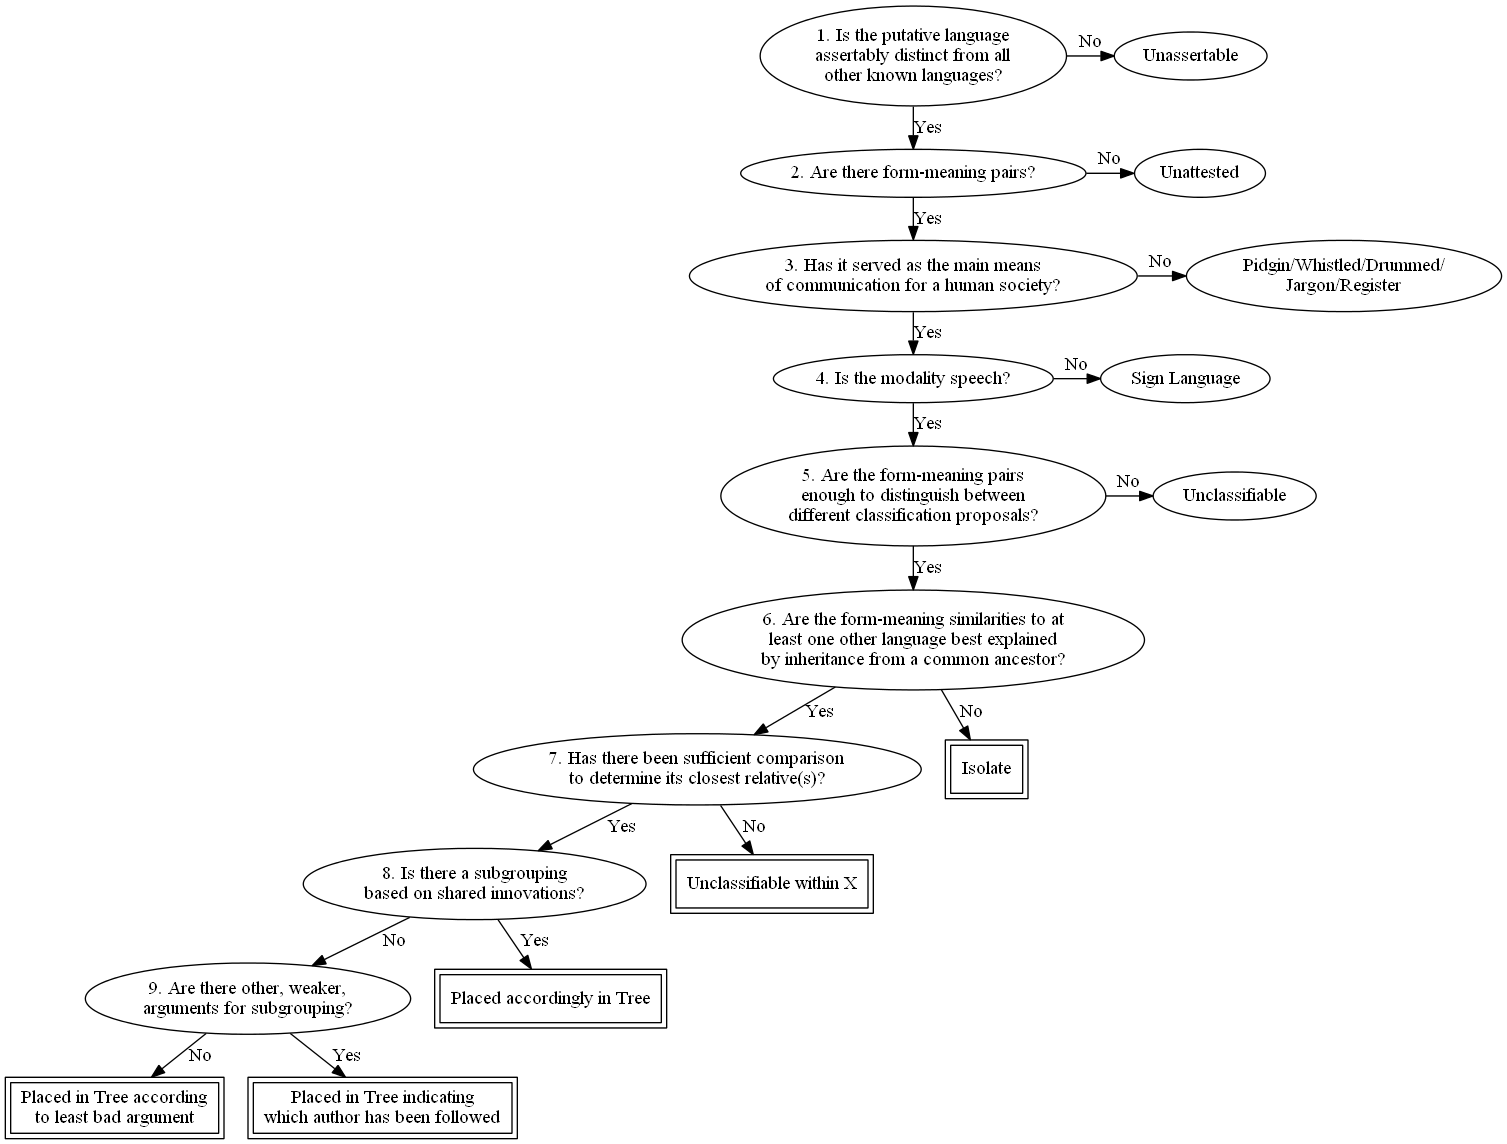
\includegraphics[width=16cm]{Glottolog_classifying_tree.png}
\caption[Decision tree for language identification and classification in Glottolog]{{Decision tree for language identification and classification in Glottolog \citep{glottologlanguoids}.}}
\label{glottolog_class_tree}
\end{figure}

In the quote above from Glottolog on ``distinctiveness'', the editors state that one can use language data and/or reports on mutual intelligibility. When empirical data on mutual intelligibility is missing, ``an approximate minimal requirement is 50 items or so of basic vocabulary'' needed for determining the distinctness of a language and where it should be placed in a genealogical tree  (\citet{glottologlanguoids} and Hammarström p.c.). This is similar to the lexical similarity measurements used by the SIL.
%and Hammarström (p.c.) has confirmed that is what is needed for distinctiveness as well (at least). SIL also makes references to lexical similarity scores, it is plausible that Glottolog and SIL International do not differ dramatically in this respect and that while the precise material and cut-off points may vary: most of the time they will end up with similar classifications for the same language varieties\footnote{In a recent paper, \citep{wichmann_2019_dialects} shows that with his new method of devising lexical similarity cut-off points, SIL tends to have a bias towards splitting rather than joining. Glottolog classifications are not tested in the paper.}. 

One important difference between Glottolog and SIL International lies in how the evidence is documented. Glottolog provides references for every language identification and tree, making it possible for other researchers to examine the evidence on their own. SIL International does not consistently provide this information. While change requests to ISO 639-3 will often refer to reports etc and many language entries have references for at least part of the information provided, there are many instances where the information is not accessible to readers. While the Ethnologue website states that ``sources used for classifications are available on request by contacting the Editor'' \citep{ethnologue2019lgident}, personal correspondence with the editors revealed that the sources are incomplete and cannot be requested in full.

Glottolog also considers whether or not the putative language has ``served as the main means of communication for a human society'' \citep{glottologlanguoids}. This disqualifies most artificial languages, whistle registers, ritual speech registers and pidgins. SIL International does not discuss this particular criteria explicitly. However, among the artificial languages Esperanto is included in the catalogue but  Klingon, High Valyrian and Angosey are not. Unlike most other artificial languages,  Esperanto does have a few native speakers \citep{bergen2001nativization}, which is probably why it is included in Ethnologue. This suggests that SIL does consider something similar to Glottolog's ``main means of communication'' criteria even if they do not spell it out explicitly. Glottolog does catalogue constructed languages, pidgins etc, placing them in so-called ``non-genealogical trees''\footnote{The list of non-genealogical trees in Glottolog are: Sign Language, Unclassifiable, Pidgin, Unattested (data missing), Mixed Language, Artificial Language and Speech Register.}. These groups of languages are included in the catalogue and given glottocodes, but the editors note that they are not subject to the same process of language identification and classification as the rest.%\footnote{It is up to Glottolog's users to filter these out of the dataset should they want to only consider languoids that are clearly classified by Glottolog's principles.}).

The fact that Glottolog provides unique stable identifiers for dialects and families, as well as languages, makes it possible to represent data in finer detail than previously possible. It also allows individual scholars to make different decisions on what is and what is not a language from Glottolog, while maintaining comparability. For example, there are several language varieties spoken on the Austral islands of the Pacific. Glottolog has classified them as being one language (Austral [aust1304]) with four dialects (Ra'ivavae [raiv1237], Rimatara [rima1237], Rurutu [ruru1237] and Tubuai [tubu1240]). However, other linguists disagree and have argued that these should be viewed as four different languages due to wordlists indicating they were not sufficiently mutually intelligible at the time of the arrival of Europeans (Walworth \& François p.c.). In this dataset, these are counted as four separate languages because it appears to be more in line with the state of the world before the arrival of Europeans. It is easy to adjust for this in the dataset (and simple to undo) because the Glottolog dialect codes are linked to the language Austral [aust1304]. 

%In this case study, I have chosen to go with the classificatory decision that these should be viewed as 4 different languages. It was easy for me to change the coding of languages in my data to include these 4 different glottocodes as separate languages instead of ``Austral'' as one. If any researcher in the future wants to make another call they can access the data and run the analysis with another classification. Since there exists glottocodes for the dialects and these are explicitly linked to their language level parent - Austral - it is easy for make the switch.

Being able to refer to dialects and families with a stable identifier is useful and an important difference between the SIL International ISO 639-3 code standard and Glottolog's glottocodes. When working with cross-linguistic and cross-cultural databases, it is often useful to be able to refer to a language variety in a more granular detail than the ISO 639-3 set allows for. \citet{nordhoff2011glottolog} point out that there may be differences between dialects that are crucial to certain research that would be confused if it was only possible to refer in a stable manner to the language level and not also to specific dialects. For example, certain dialects of German make a distinction between /e:/ and /æ:/ whilst others don't. If references were not accurately tied to a language variety, this would be confusing as ``German'' would have different numbers of vowels in different sources. By providing stable identifiers for dialects as well as languages and providing a controlled hierarchy, it is possible for researchers to document their data accurately while still making it possible to aggregate up to the ``language-level'' when it is desirable. For example, Grambank and the Standard Cross Cultural Sample of D-PLACE both contain entries for specific languages and dialects. There are 158 one-to-one matches between the glottocodes of these two databases. In some cases though, the databases contain different dialects of the same language. If we were to lump dialects of the same language together in each of the datasets, the overlap increases to 183.

The definitions of language in ISO 639-3 (as described in Ethnologue \citep{ethnologue2019lgident}) and Glottolog both focus on mutual intelligibility. Ethnologue notes that intelligibility does have to be symmetric, but neither of the resources discuss multilingualism, or multidialectalism in any detail. It is possible that the world used to be much more multilingual than it is today \citep{evans2017did}, and there are still many places where communities are highly competent in many different language varieties. Ethnologue state that they focus on \emph{inherent} intelligibility, as opposed to \emph{acquired}, but in situations where languages are not formally taught but rather present in the community continuously it can be difficult to draw the boundary between inherent and acquired. The underestimation of multilingualism has significant consequences for studies of the evolution of language \citep{roberts2013evolutionary}. However, unless two languages are exclusively spoken in a fully multilingual setting and never outside of it, the total count of languages should remain the same. 

%It is not within the scope, or indeed even the aim, of the present study to provide a universal and unproblematic classification of languages. 
The language classification standards for Glottolog and SIL International do differ conceptually, and many of their differences may reflect their different aims (facilitating academic research by making references more accessible and integrated as compared to facilitating description and translation of the Bible into the world's languages). However, the counts for languages in the world that they produce are not that different in the end.

I will be using the classification of Glottolog, with a few adjustments, since it is more transparent and better referenced. It should be noted that using the ISO 639-3 results in the language count for the Vanuatu being 108, as opposed to 105 in Glottolog, which is not a huge difference. 

The aim of this study is to explore language diversification in Remote Oceania prior to the arrival of European people. Because of this, I have made a few adjustments to the Glottolog classifications of languages in the relevant region. Languages that have come into the region directly because of the arrival of Europeans have been excluded (Bislama, English, French etc). Furthermore, I have made three other changes from Glottolog in the classification of indigenous languages of the region based on other accounts of their mutual intelligibility at the relevant point in time\footnote{Tahitianization and dialect/language levelling has occurred, and therefore languages that used to be more different from each other are now more similar.}. Firstly: in Fiji, Glottolog's Eastern Fijian [fiji1243] is split into three languages: Southeast Fijian [sout2864], Northeast Fijian [nort2842] and Kadavu [kada1285] based on personal correspondence with Andrew Pawley and Paul Geraghty. Secondly, M\={a}ori [maor1246] is split into two languages: Morori [mori1267] on R\={e}kohou (Chatham Islands) and M\={a}ori [maor1246] on mainland Aotearoa (New Zealand). This classification is based on \citet{harlow1973regional} and personal advice from Andrew Pawley. Third and finally, as was previously mentioned, the languages of the Austral Islands have been divided from one to four based on advice from Mary Walworth and Alexandre François.

The splitting of Eastern Fijian [fiji1243] into three languages has as consequence that the total language count for Fiji as one island group based on overnight sailing distances is 8 instead of 5. When the island groups are defined in relation to whether they share at least one language, the great island of Viti Levu is paired with Yasawa into one group sporting 4 languages instead of 2 and Kadavu separates out as a separate island group with 1 language. For M\={a}ori [maor1246] the difference in language classification makes less difference. Aotearoa and  R\={e}kohou were always separated as different overnight distance island groups, each sporting one language (even though it is the same language under Glottolog's definition). For the island groups based on shared language they continue to be separated under the new classification, meaning in practice that we have yet another small Polynesian island group with one language. The situation is similar for the Austral islands. The new classification makes no difference for the island groups as defined by overnight distances, since all four are separated out from each other already. For the island groups based on shared language they continue to be separated out as different island groups. Overall the new classification results in more languages in Fiji, and more small Polynesian island groups with one language each.


\FloatBarrier
\subsubsection{Grouping Islands and atolls}
\label{sec:island_geo}
%polygon_plot_SBZR

%When measuring language diversity, many methods do not deal well with islands and water. For example, all islands with only one language were excluded from the study by \citet{curriemace2009} on the relationship between language territory and ethnographic features. This is unfortunate, but understandable. The authors model of language diversification was not able to accurately enough deal with contact over water.

For this study, we need a good way of grouping islands and atolls in Remote Oceania (5,525 landmasses) that is not dependent on modern politics (e.g. nation states), but that reflects possible meaningful networks in Oceania prior to colonization. For this purpose, we will use two distinct approaches. The first is based on voyaging distances by canoe, and the second is based on whether the islands have a language in common or not. The assumption is that a group of islands is a meaningful unit for comparison if it forms a significant \textit{network of contact} and that this can be approximated by shorter sailing distances or evidenced by the maintenance of a shared language. 

These two principles, overnight sailing distances and sharing a language, have been applied consistently over all islands and all languages using data available in the Ethnologue \citep{ethnologue22}, Glottolog \citep{glottolog3} and in some cases specialist literature (\citet{faaniu1983tuvalu,charpentier2012linguistic, francoisetatl2015, macdonald_2020, omniglot_tuvaluan} and a map of indigenous languages of New Caledonia published by CNRS-LACITO). For more on the definition of languages, see section \ref{sec:language_class}.


%\citet{hauofa_1993}

%\citep[194]{irwin1994prehistoric} inter-island vogagýing existed and micronesian atolls are precarious

\textbf{Grouping islands based on voyaging distances}. \citet{mark_1986, marck2000} has suggested that islands within 100 miles\footnote{Note that Marck uses \emph{land} miles, not \emph{sea} miles (Marck personal correspondence).} are reachable by overnight voyages in a traditional canoe (24h). This is taken to represent a good approximation of island connections of frequent contact and is supported by other accounts, such as \citep[38]{gladwin2009east} who notes a higher frequency of travel between islands within 100 miles of each other. This is a distance people may travel for tribute offerings, trade and community events, which strengthens cultural ties. Further away, and it may not be so easy to get together as often. Fig. \ref{Marck_2000_east_poly} shows this principle applied to central East Polynesia.

\begin{figure}[ht]
\centering
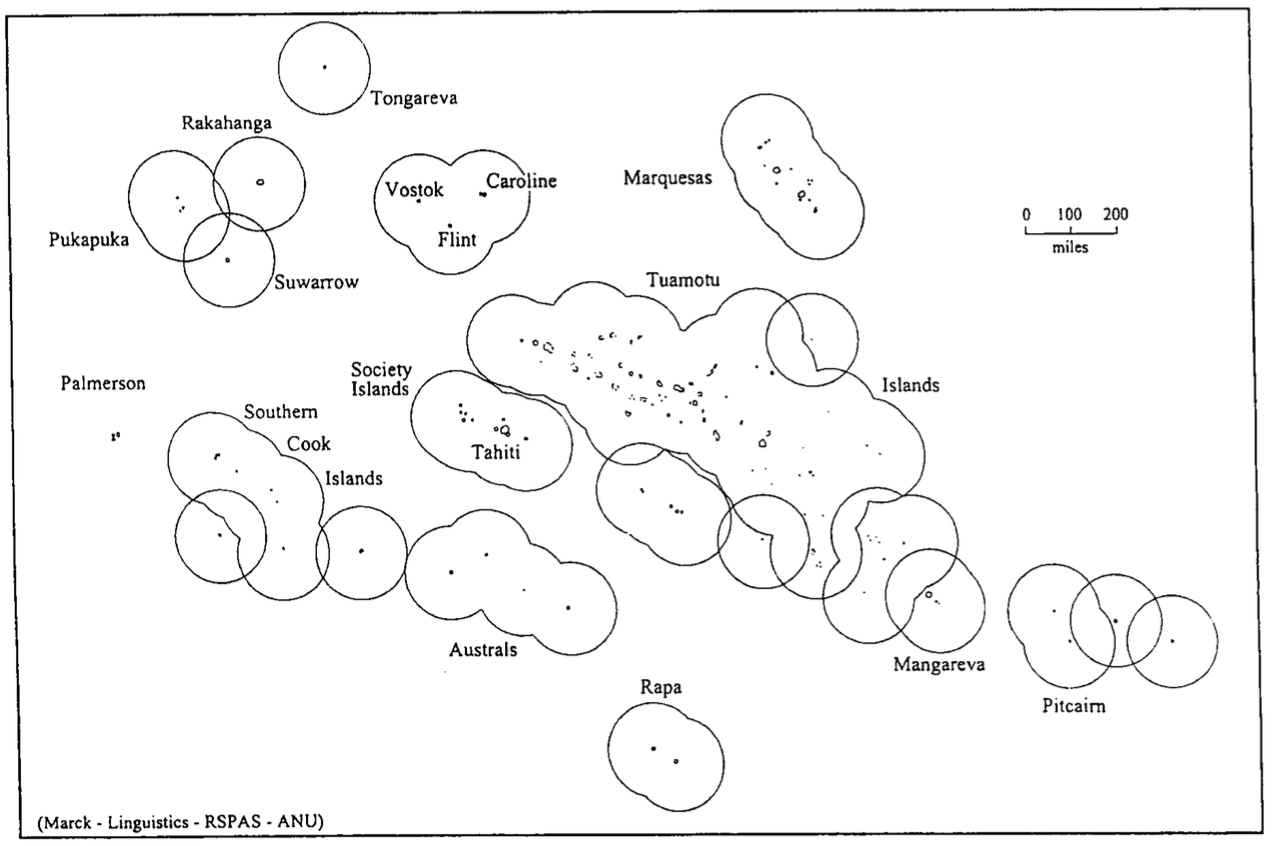
\includegraphics[width=13cm]{marck_2000_east_poly.png}
\caption{{Map of central East Polynesia from \citet{marck2000}, showing 100 mile radii.}}
\label{Marck_2000_east_poly}
\end{figure}

This idea proved useful also in terms of understanding language communities. \citet{mark_1986, marck2000} demonstrates that this way of grouping islands often conforms neatly to linguistic boundaries --- especially in the north and east Pacific. For example, in Fig  \ref{Marck_2000_east_poly} the boundaries mostly line up well with well-established linguistic boundaries (with some exceptions, such as Tuamotus being split Australs merged etc). These island groups also line up somewhat with the ``interaction spheres'' in East Polynesia identified by \citet{rolett2002voyaging}\footnote{\citet{rolett2004environmental} consider islands within 50 km of each other as a meaningful unit, but do not extrapolate on why this is.}. 

However, this way of grouping islands does not take into account currents and winds - they are ``just'' a simple 100 mile distance straight from the coastline. \citet{NZSA_overnight_2023} improved upon this initial idea by incorporating a cost-surface that accounts for wind, currents and canoe profile shapes. The canoe that was used to model the distances was a v-shaped outrigger, see Fig. \ref{kane_fishing_canoe}. The results were largely similar, strengthening the assumption that 100 miles is a decent approximation. It is this latter island grouping that we will use in this study. We will refer to these island groups as \textit{overnight distance groups}. Fig. \ref{polygon_plot_SBZR} shows this grouping, along with the number of languages per group. Out of the 56 island groups of this kind that were possible to include in the analysis, 45 have only one language.

\begin{figure}[ht]
\centering

\includegraphics[width=10cm]{Herb-Kane_Fishing-Canoe-off-North-Kona.jpg}
\caption{{The painting ``A Fishing Canoe off North Kona'' by Herbert Kawainui K{\=a}ne. Illustration of an outrigger canoe with v-shaped hull. Copyright Herbert K. K{\=a}ne, LLC.}}
\label{kane_fishing_canoe}
\end{figure}

\begin{sidewaysfigure}[p]
\centering
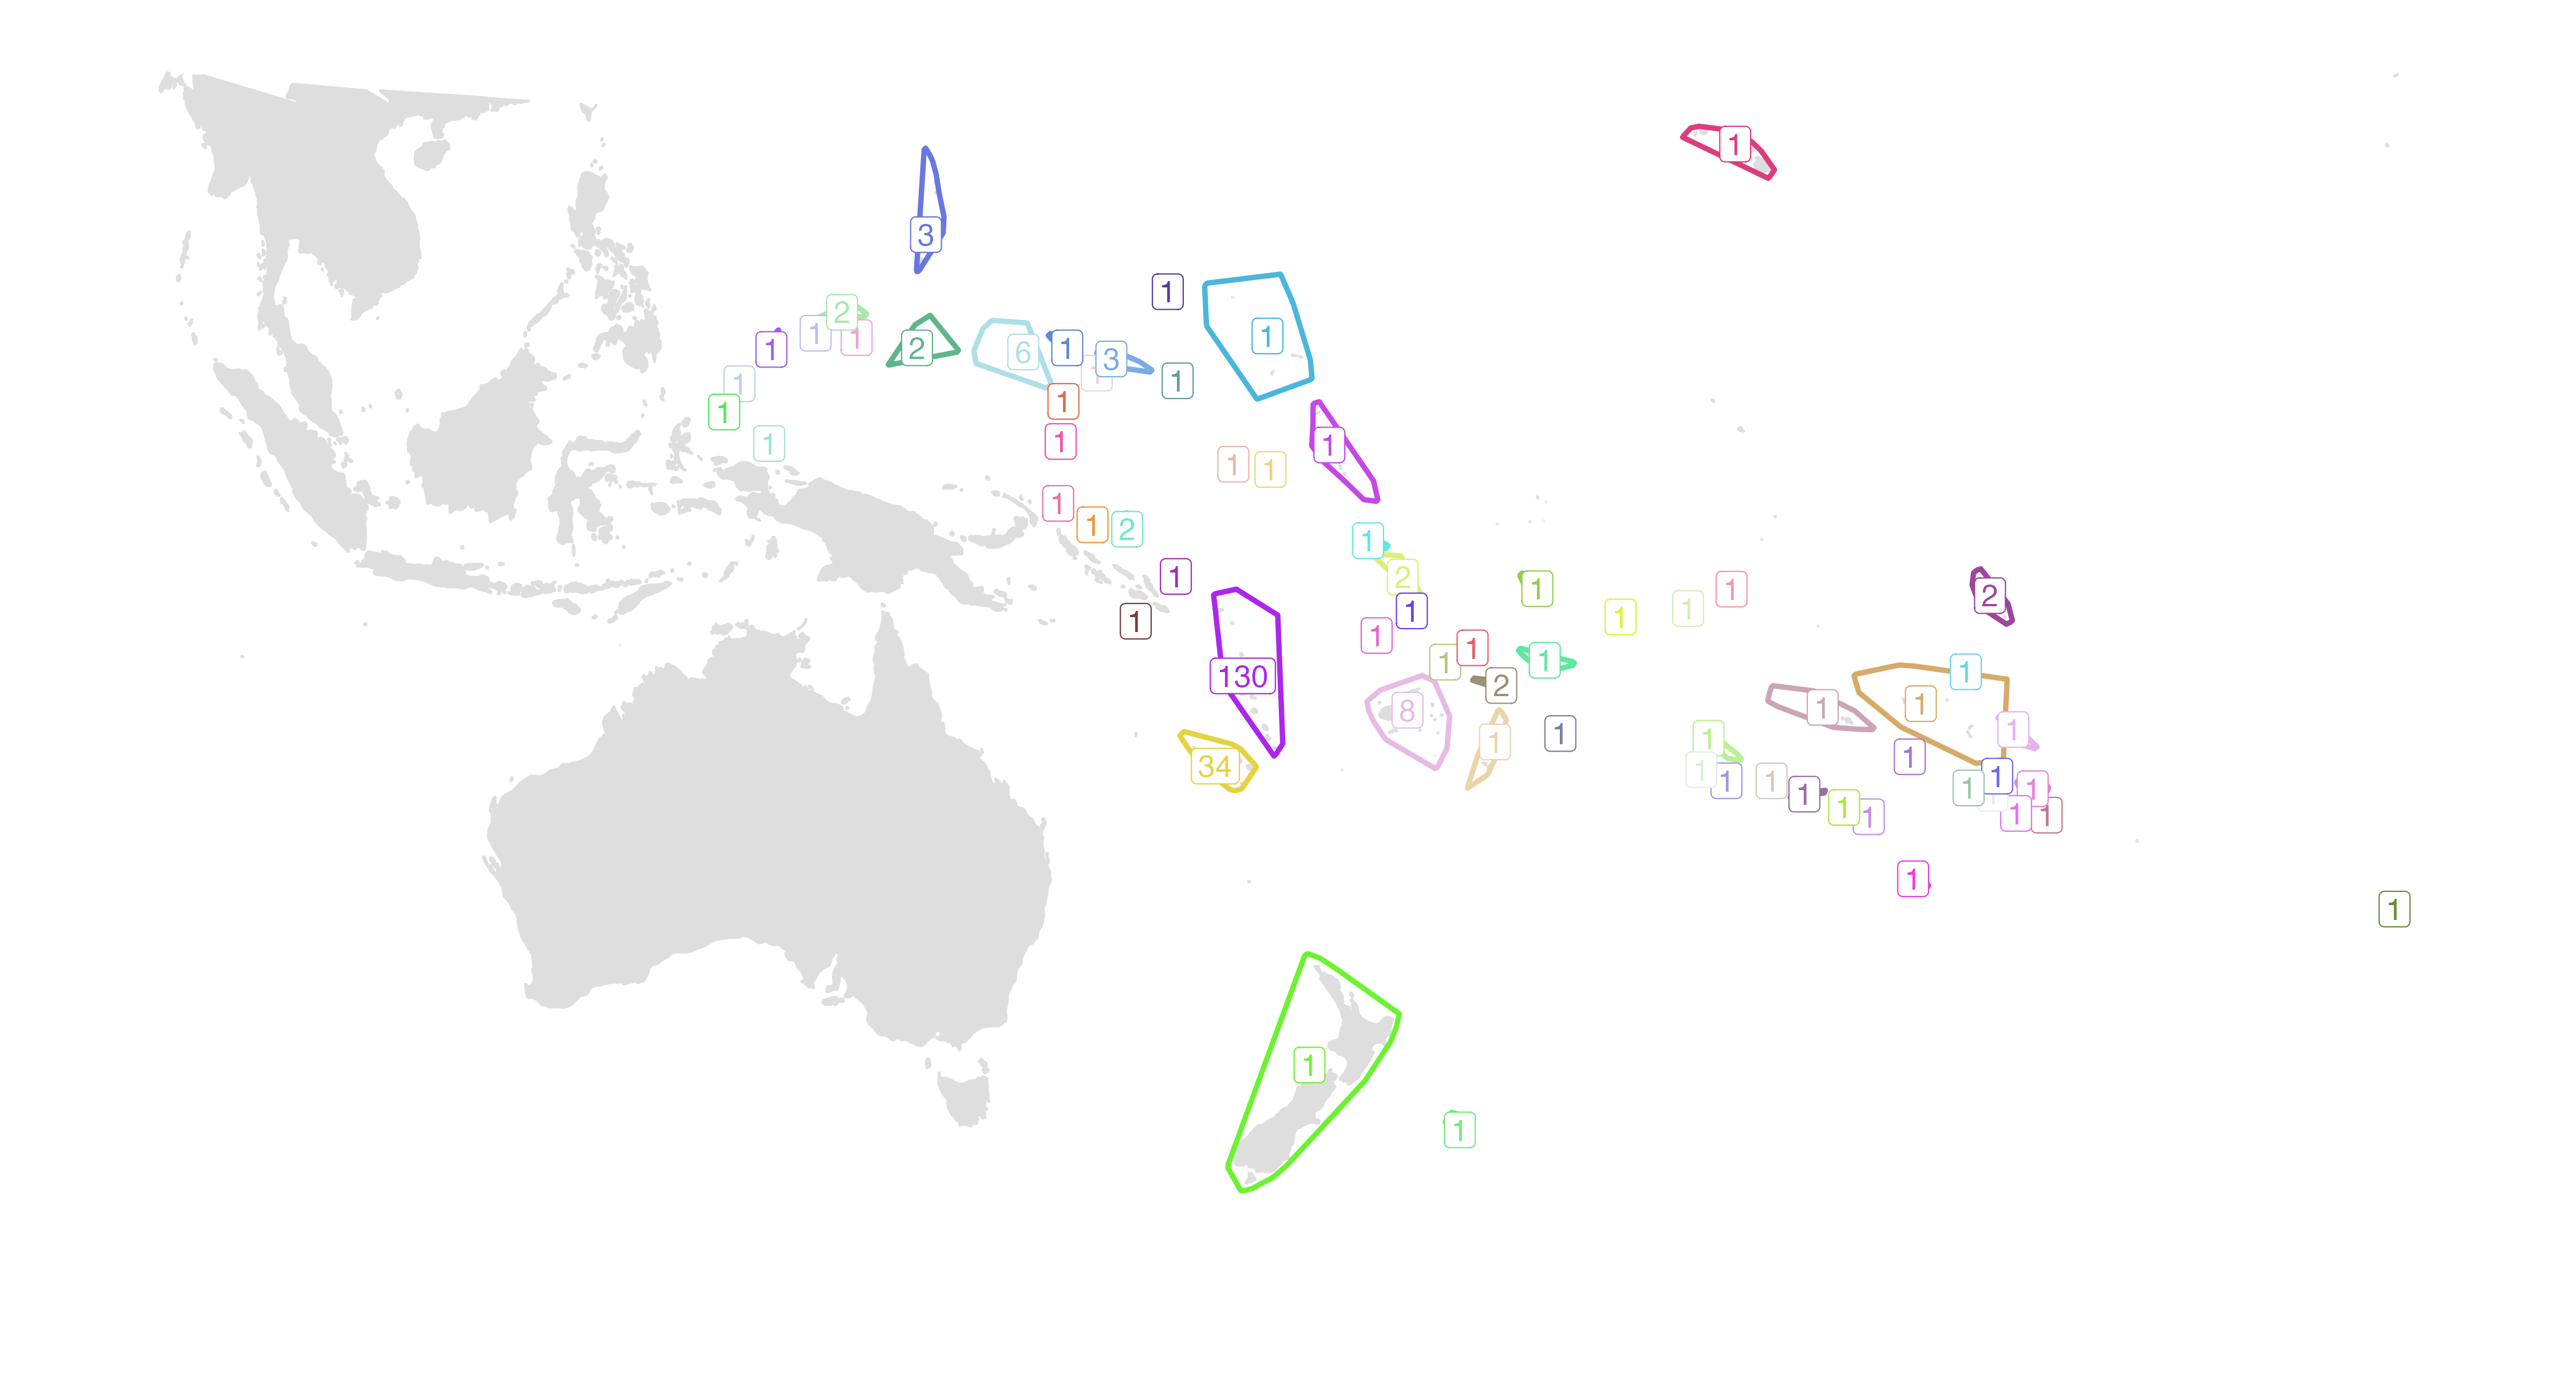
\includegraphics[width=\textwidth]{polygon_SBZR_group_map.png}
\caption{{Distribution of languages per overnight sailing distance island group.}}
\label{polygon_plot_SBZR}
\end{sidewaysfigure}



\textbf{Grouping islands based on (at least one) shared language}. If two islands share a language, they are classified as of the same island group. For example, all islands of the Tuamotu archipelago (where Tuamotuan [tuam1242] is spoken) are merged, even though they are grouped into several separate island groups by the overnight distance approach. Vanuatu, being a land of great language diversity, has a different group for almost every island. Another example is the Tungaru islands (western islands of modern-day Kiribati) and Tuvalu which actually share a language. Most people of the country of Tuvalu speak Tuvaluan, but there is one island, Nui, where Tungaru (Gilbertese [gilb1244]) is also spoken \citep{faaniu1983tuvalu, macdonald_2020, omniglot_tuvaluan}. We will call these island groups \textit{shared language groups}. Fig \ref{polygon_plot_medium} shows these groups, and their language counts. Out of the 65 island groups that were included in the modelling, 21 had only one language.

\begin{sidewaysfigure}[p]
\centering
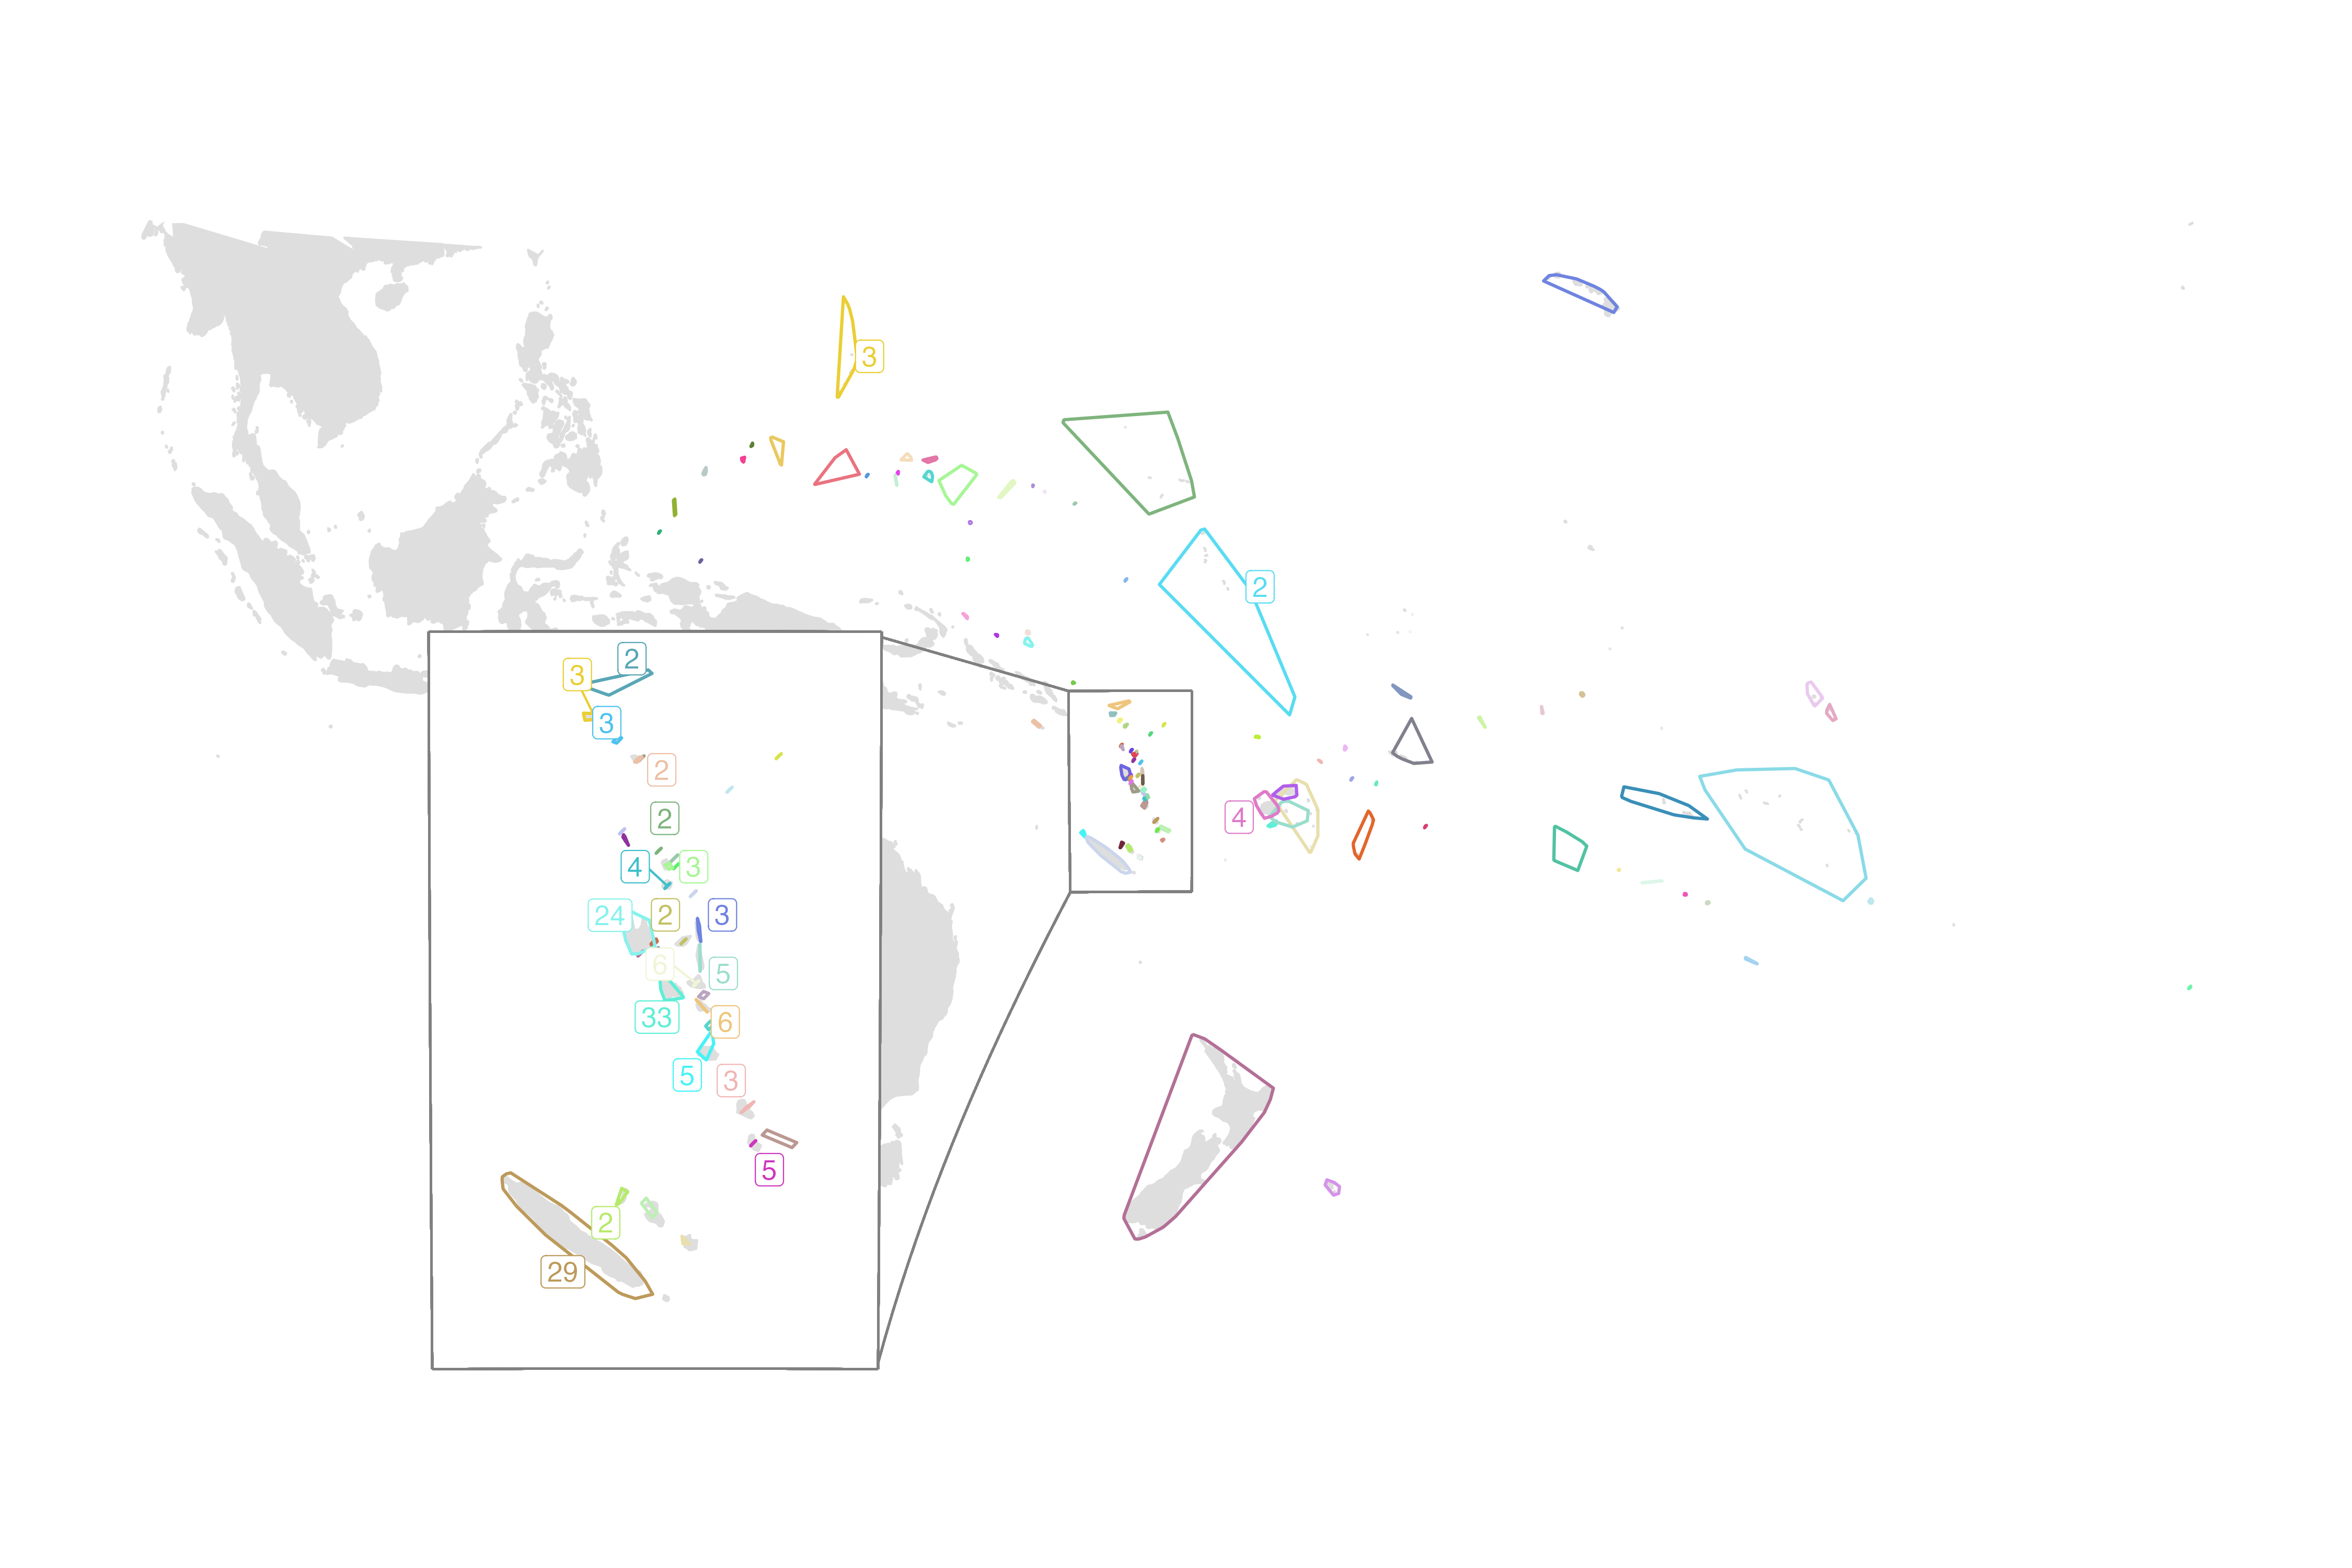
\includegraphics[width=\textwidth]{polygon_medium_group_map_vanuatu_mh_inset.png}
\caption{{Distribution of languages per shared language island group. Island groups with only one language do not have a label as this cluttered the visualisation. All island groups without a label have 1 language.}}
\label{polygon_plot_medium}
\end{sidewaysfigure}

Finally, these island groups should be taken with a grain of salt. They are most likely better than using modern nation-states and they are more explicitly and principally defined than many other island groups in other studies which rely on conventional definitions of well-known island groups or consider each island separately. However, the task of finding definite meaningful social geographic units in Oceania prior to colonization is difficult. Most likely the parameters vary over the space, for example with access to different kinds of sailing technology or different customs. Furthermore, from the initial settlement of Remote Oceania approximately 3,000 years ago until Western colonisation, there must have been a large amount of variation. \citep{rolett2002voyaging} for example discusses the decline in inter-island group voyaging in East Polynesia after 1450 CE. That said, these two approaches offer two different ways of viewing Oceania as socially interconnected space --- one more granular than the other --- and are the best available island groupings for historic research.



%\footnote{This map has been produced by the team of Oceanic linguists at CNRS-LACITO, but it has never been officially published. It appears in other academic papers, for example \citet{speedy2013reflections}, but regretfully it is not possible to provide a stable bibliographical reference to it independently.}.
%For each of these island groups, absolute latitude, total area and shoreline were calculated from the Global Self-consistent, Hierarchical, High-resolution Geography Database (GSHHG), version 2.3.7 \citep{wessel1996global}. The analysis of this study also includes the ratio of shoreline to area, as we may expect islands groups with many small islands and atolls to be different from those with one large island, even if their overall area is the same\footnote{Thank you to the anonymous examiner who suggested including this.}. Area and shoreline were both log-transformed (log 10). This was done both to be in line with previous studies \citep{gavin2012island} and because the distributions had extreme outliers (New Caledonia and Aotearoa/New Zealand). Such outliers end up driving the model in a manner that is not representative of the overall sample. By logging these variables the overall structure and order of data-points remains the same but the influence of the extreme outliers is reduced.

%ANU CartoGIS also provided data for the water area which is covered by the overnight sailing distances, the light-blue shaded areas of Fig.~\ref{RO_overnight_coloured_dots}.The area between and around islands is important because it provides access to fish and seafood (c.f. rice or wheat fields to agriculturalists or tundra and taiga to reindeer herders), islands which have less territory of this kind but equal land area to another island may be able to support fewer people. For the island groups defined by shared language which are smaller than Marck groups, the water area was assigned proportionally to the islands landmass size in comparison to the entire Marck group's landmass (i.e. Malakula makes up)

%A score of isolation was also calculated based on the GSHHG-data as well. There are many different ways of measuring island isolation. \citet{rolett2004environmental} use two measures, distance from home island to island which is >25\% larger than home island and distance to island >75\% larger than home island. \citet{gavin2012island} use distance to the Asian continent (after considering three other measurements). The ``Isolation index'' of the Islands database \citep{dahl1991island}  is calculated as follows: (distance to nearest equivalent or larger island)$^{0.5}$ + (distance to nearest island group or archipelago)$^{0.5}$ + (distance to nearest continent)$^{0.5}$. \citet{weigelt_2013} present an overview and comparison of 17 different island isolation measurements used in biology and conclude that it is advisable to consider stepping-stone pathways, larger islands (besides continents), climatic similarity and the area of surrounding landmasses when studying the richness of species in relation to island isolation.

%In light of this, and given the data available, a simple isolation metric has been calculated. This measurement consists of \textit{the distance from the largest landmass of each island group to the closest landmass which is the largest in its island group}. This is essentially a distance of ``home island'' to closest other ``home island''. For example, for Hawai'i the largest island is the Big Island. The closest island to the Big Island which is also itself the largest in its group is part of the M\={a}ngarongaro atoll (also known as Penrhyn or Tongareva). This distance is 3,191 km. This is the largest distance for our isolation measurements, therefore Hawai'i is the most isolated island group. The metric is calculated separately for the overnight distance groups and shared language groups and was also logged (log 10) for the same reasons that area and shoreline was logged.

Each island group is associated with the languages spoken there, based on information in the various sources cited earlier for defining groups by shared language. Naturally, some islands will have many languages assigned to them, most notably Santo and Malakula in Vanuatu with 24 and 33 languages respectively. Other languages are spread out over many islands and atolls. Tuamotuan [tuam1242] is for example assigned to 1,302 distinct landmasses (in this dataset atolls and reefs that are above water appear as several small landmasses). For shared language groups, these landmasses are all joined under the label `Paumotu'. However, as defined by overnight sailing distances this archipelago is split into several different island groups each with one language. The fact that it is the same language is not accounted for (\citet{gavin2012island} also arrange their data like this).

\FloatBarrier
\subsubsection{``Political complexity''}
\label{appendix_def_pol_complex}
The hypothesis tested in this study relies on a systematic measure of political structure across societies. The most widely used variable in this regard is variable 33 of the Ethnographic Atlas \citep{EA_1971}: ``jurisdictional hierarchy beyond local community'' (EA033). This section gives an overview of how this variable is defined and its distribution in Remote Oceania. 

The Ethnographic Atlas was first published in 1962 and is one of the datasets included in D-PLACE \citep{d_place_all}. EA033 is widely used to represent ``political complexity'' in studies of cultural evolution. This variable has been used to study the relationships between language area, subsistence strategies and political organisation \citep{curriemace2009}; processes of rise and fall of ``political complexity'' in South-east Asia and the Pacific \citep{currie2010rise}; the spread of Christianity in the Pacific \citep{watts_2018}; and co-evolution of intensive use of natural resources and political structure \citep{sheehan2018coevolution}.  

In all of the studies referenced above, EA033 is used as a way of quantifying vertical political structure within a given society beyond the local community. In the rest of this study we will be referring to this variable as ``political complexity''. There is a separate variable (EA032) for jurisdictional hierarchy \emph{within} local communities. This variable could not be included due to missing data. 

``Local community'' is in the ethnographic/anthropological literature is defined as the ``maximal group of persons who normally reside together in face-to-face association'' \citep{yale1945outline}. The size and distribution of local community may vary greatly. For Remote Oceania, the Ethnographic Atlas records entries ranging from less than 50 (Ponape) to between 400-1000 (Tikopia).

``Society'' is not defined explicitly in most of the literature, but it is sometimes used interchangeably with ``ethnic group'' or ``culture''. \citet{roger1981cultural} write:

\begin{quotation}
\noindent\emph{[A]ll the communities that are connected politically and economically (and hence comprise a kind of total social system) can be taken as comprising a \textbf{society}. Characteristically, a society comprises a total social system whose members share a common language and cultural tradition}. 
\begin{flushright}
\citep[22]{roger1981cultural} \footnote{Ironically, later in this section \citet[23]{roger1981cultural} quote \citet[422]{schwartz1978culture} in saying that the ``Manus people'' as a society are easily linguistically bounded, when linguists have counted up to 19 languages on the island \citep{glottolog40}. In D-PLACE \citep{d_place_all} the society ``Manus'' in the Ethnographic Atlas is specifically linked to one language out of these 19, Titan [tita1241].} 

\end{flushright}
 \end{quotation}

It is not possible to give more detail to the definition of ``society'' as employed in the Ethnographic Atlas dataset, but it does seem to correspond to ``language community'' to a great extent. In cases where societies are multilingual (c.f. \citet{evans2017did}), it is less likely that the definition relies on one shared language. It is, however, unclear how such cases are represented in the Ethnographic Dataset.

In some instances, it may be that ``local community'' and ``society'' are one and the same. For example, the total population for the ``ethnic group'' (variable EA202) of the society Tikopia is 1,300 which is not that much larger than the mean size of the local community (EA031) noted above. On the other hand, the total population of the ethnic group of Ponape is 8,000, which would result in an estimate of 160 local communities given the value of mean size of local community (EA031).
  
Political complexity (EA033) as a variable is observed per society, i.e. it does \emph{not} capture relationships \emph{between} distinct societies. It also does not track the political structure \emph{within} the local community\footnote{Ethnographic Atlas variable 32 captures jurisdictional hierarchies \emph{within} local communities.} or \emph{horizontal} political relationships within a society (e.g. political relationships between equal genealogical groups). It specifically measures \emph{vertical} jurisdictional levels \emph{within} a given society, \emph{beyond} the local community. Furthermore, it targets ``jurisdictional'' authority --- not just the existence of rank. In other words, the levels of authority need to be tied to some kind of jurisdictional power, most likely the power to exert punishment for transgressions and the possibility to declare war upon other societies. 

Specifically, it is necessary to underline that despite the common name for this variable in the Ethnographic Atlas --- ``Political complexity'' --- it does not include politically complex systems such as the Kula exchange ring\citet{damon2002kula}, see Fig \ref{kula_ring}. Exchange systems of trade/debt are definitely complex and political, but they are not included in EA033 as they do not track \emph{vertical} complexity.

\begin{figure}[ht]
\centering
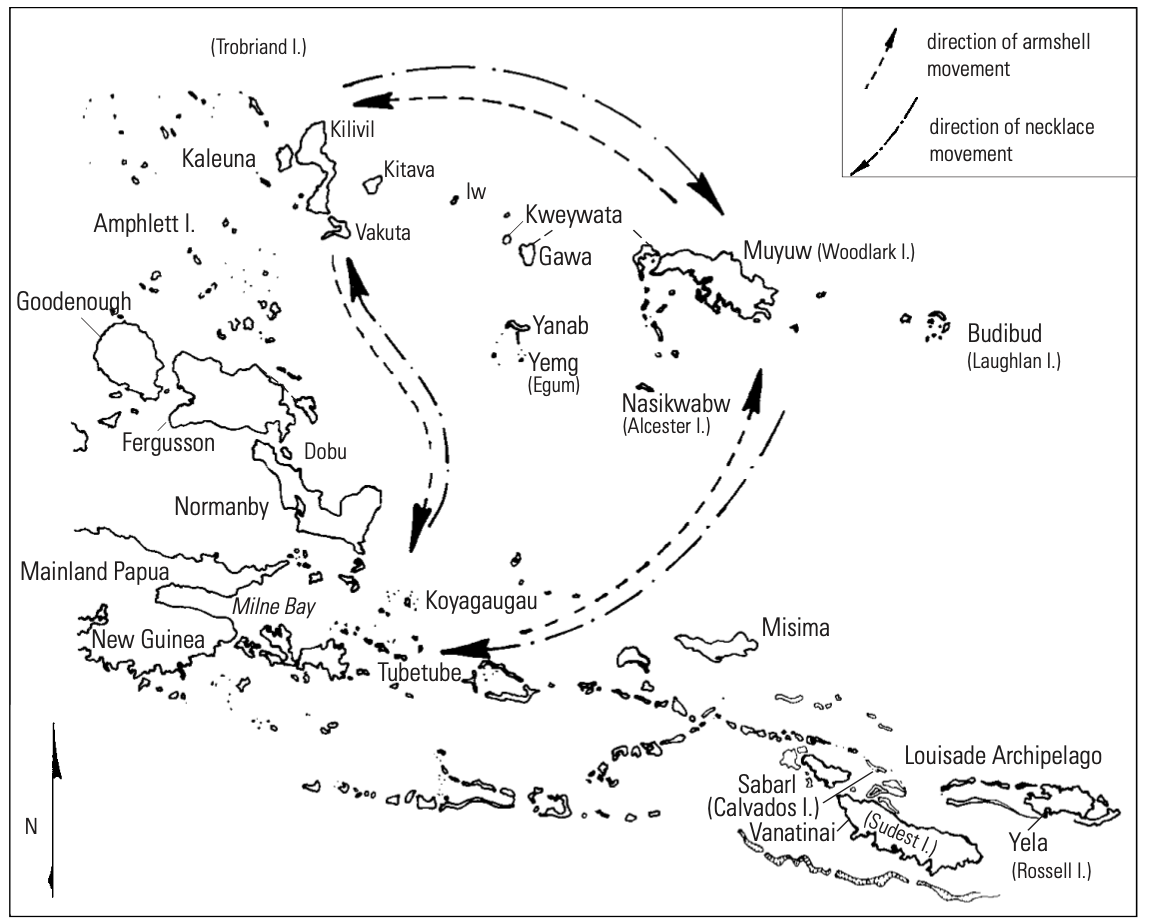
\includegraphics[width=10cm]{latex/kula_ring_damon.png}
\caption{Kula exchange ring, from \citet{damon2002kula}.}
\label{kula_ring}
\end{figure}


The possible values societies can take for this variable of political complexity are:

\begin{enumerate}
\item No levels (no political authority beyond community)
\item One level (e.g., petty chiefdoms)
\item Two levels (e.g., larger chiefdoms)
\item Three levels (e.g., states) 
\item Four levels (e.g., large states)
\end{enumerate}

\citet{giuliano2018ancestral} write: 

\begin{quotation}
\noindent\emph{[I]f the local village chief is the highest level of authority, and he or she does not answer to anyone above them, then the variable would take on a value of [1]. If above the chief, there was a district leader, then above this, there was a territory leader, and above this a provincial leader, and above this the paramount chief, then this variable would take on the value of [5].} 
\begin{flushright}
\citet[9]{giuliano2018ancestral}
\end{flushright}
\end{quotation}

This way of characterising political structure aligns well with ethnographic accounts of political structures in Western Polynesia, as we have for example seen in descriptions by \citet{sahlins63}. Consider Fig.~\ref{meleiseapyramid} \citep[22]{meleisea1995} for example, which illustrates the ideal characterisation of political power in S\={a}moa. The village level (\emph{matai} titles) corresponds to value 1 for EA033, subdistrict (\emph{ali'i} titles) level 2, district level (\emph{ali'i pa'ia / ao} titles) 3 and nation (\emph{tafa'if\={a} / tupu} titles) corresponds to level 4. S\={a}moa is however coded as level 3 since paramount titles are very unstable in the archipelago, even though they theoretically do exist.

%\footnote{There exists some variation in the literature as to where to start this scale, either with 1 = no political authority beyond community, or 1 = missing data. We will be using the default scale in the Ethnographic Atlas Codebook from \citet{gray1998ethnographic} here and adjust quotes from other publications to this scale so as to reduce confusion.}

\begin{figure}[ht]
\centering
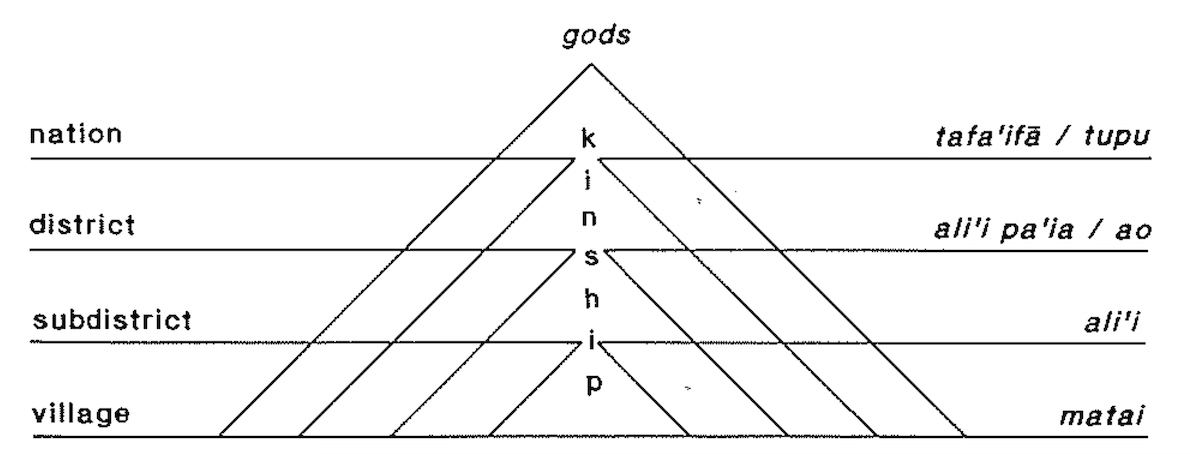
\includegraphics[width=13cm]{pyramid_meleisea.png}
\caption[Illustration of traditional political organisation of S\={a}moa.]{{Illustration of the traditional political organisation of S\={a}moa from \citet[22]{meleisea1995}.}}
\label{meleiseapyramid}
\end{figure}

However, this framework is less easy to apply to the Melanesian islands of Remote Oceania where political structure often is described more in terms of autonomous and equal groups organised into horizontal structures such as exchange networks --- both within and between societies (c.f. \citet{bonnemaison1996graded} and \citet{huffman1996trading}). \citet{bolton1998chief} points out that the very concept of ``chief'' is new to Vanuatu, writing that chiefs were first introduced by Europeans to fill the role of ``representative for a community towards outsiders'' and then transformed into ``representative for traditional culture (kastom)'' \citep[185]{bolton1998chief}. In this study, political complexity is assumed to be a proxy measurement of social network cohesiveness (c.f. \citet{grace_1992_aberrant}). Differences between modern Vanuatu ``chiefs'' and pre-European political structures are therefore unlikely to be large enough to give rise to dramatically different scores in this metric. As has been shown in previous studies, while this metric may be coarse grained and not capture all the nuances of political life in the region, it appears to still be useful in testing hypotheses such as the one investigated in this study.

%, it may still be valuable to us in a) operationalising the hypothesis of Turner/Sahlins/Pawley

%Given this, what does it mean to go looking for ``chiefs'' and ranks in Vanuatu and what would descriptions of such institutions in ethnographies actually capture?

%Problematic as this variable may be in faithfully capturing relevant facts of political structure in all the societies in our sample, it may still be valuable to us in a) operationalising the hypothesis of Turner/Sahlins/Pawley and b) capturing something about social networks and group identity (even if it only measures this by proxy). In this case study, we are testing the hypothesis that societies that are rules by ``powerful chiefs'' and have more levels of vertical jurisdictional structures are slower at diversifying than societies with a more egalitarian/horizontal structure. Given that this is what we are testing, I believe that variable EA033 can still serve us well even if it does not capture the nuances of power structures equally well throughout the region.

Given our language classification earlier, there are 233 language communities in our maximal sample. The ethnographic data is collected per society, and as was mentioned earlier it is possible for different societies to have the same language. Societies with the same language have been merged and our smallest cultural units of analysis are the language-society\footnote{American S\={a}moans and Upolu S\={a}moans were the only societies that needed merging in this fashion.}. Each language is associated with the islands and atolls where it is described as spoken. The full geographical dataset contains 5,525 unique landmass polygons\footnote{The total number of polygons in the geographical dataset is 9,750, but this includes New Guinea and uninhabited islands (Phoenix Islands for example). 5,525 is the number of unique polygons that can be associated with a community of Remote Oceania.} which have been grouped into our smallest geographical unit of analysis: 104 shared language island groups. In the analysis, we will also be aggregating the islands into 69 overnight distance groups.

D-PLACE has a value recorded for political complexity for 44 ``language-societies'' in Remote Oceania. There have also been more recent studies where other authors have added more entries. We will be using additional data-points from a separate publication by \citet{sheehan2018coevolution}, resulting in another 27 data-points. There was an overlap between these two datasets, 26 language-socities having a coding both in the original Ethnographic Atlas dataset in D-PLACE and in Sheehan et al. Of these, 11 societies (i.e. 43\%) were coded exactly the same. Upon closer investigation of the instances where the coding differed, I found that Sheehan et al often had access to \textit{more} data, more \textit{comprehensive} data and more \textit{recent} data. Each of these instances was re-evaluated, and most often the coding from Sheehan et al was kept\footnote{I am grateful to Sheehan for very helpful personal correspondence during this process.}. The data was also further supplemented with information from \citet[201]{bonnemaison1996graded}, resulting in 66 more data-points in Vanuatu. 



%For the instances where they had represented the same society with different values, I consulted the relevant ethnographies myself and made my own coding decision. In the most cases, my evaluation of the data sided with the interpretation by Sheehan et al. Given that Sheehan et al have access to more recent and more comprehensive ethnographic material, it shouldn't be surprising that they have made different decisions and that a second look is more likely to agree with their evaluation than the older dataset. 

%Reading ethnographies is difficult, and involves a lot of interpretation and additional knowledge of context. It is not that dissimilar from reading grammars (which I have more experience with). If anything, reading ethnographies is tricker than reading grammars since there is more variation in how to describe ``a culture'' than there is on how to describe ``a language''. I had the fortune to be able to correspond with Sheehan and discuss particular cases in greater detail, which was very valuable. During these investigations, I also came across a typology of political systems in Vanuatu compiled by \citet{bonnemaison1996graded} (see Fig.~\ref{Bonnemaison_map}) which provided more data-points. In reading \citet{bonnemaison1996graded, sahlins63},  and discussing with Sheehan, I concluded that it is possible to infer a level of 1 for EA033 where Bonnemaison describes a society as having a ``grade-taking system''. It is however unclear if a coding of 2 or higher can be made when societies are described as ``chieftainship of ``Polynesian'' type, so I did not record those observations in our dataset. In the end, I arrived at a dataset that had good enough coverage for this study (130 out of 233 language-societies and 61/105 island groups) and that I felt confident represented the description of these societies well. 

%\begin{figure}[ht]
%\centering
%\includegraphics[width=13cm]{Bonnemaison_1996_vanuatu_map.png}
%\caption{{Map of traditional systems of power in Vanuatu, from \citet[201]{bonnemaison1996graded}.}}
%\label{Bonnemaison_map}
%\end{figure}


It should be noted that this data does not represent the state of these societies for the entire period between first settlement and European arrival. As \citet{meleisea1995} writes, anthropology of the Pacific often depicts an unrealistic ``ethnographic present''. For example, \citet[185]{schoeffel87} writes about the shift in the political world of S\={a}moa under the rule of Salam\={a}sina which gave rise to a greater distinction between two kinds of chiefs: \emph{tul\={a}fale} and \emph{ali'i}. \citet[249]{kirch2017road} also mentions this distinction, but notes that it mainly came to prominence in the 1500's. As a way of avoiding this problem, the D-PLACE database \citep{d_place_all} contains information on the focal years of the description. The data for the variable on political complexity in Remote Oceania varies from 1800 (Hawai'i) and 1940 (Vanua Levu). This study assumes that even more recent data may sufficiently accurately reflect the state of past societies, such that it remains useful for testing the central hypothesis.

Fig.~\ref{pol_complex_map} represents the coding of political complexity for the relevant societies. A more detailed table can be found in appendix \ref{appendix_pol_complex}. While it is indeed the case that societies of Melanesian Remote Oceania tend to have lower levels of political complexity, it should be noted that many societies in Polynesia and Micronesia also score a value of 1.

\begin{sidewaysfigure}
\centering
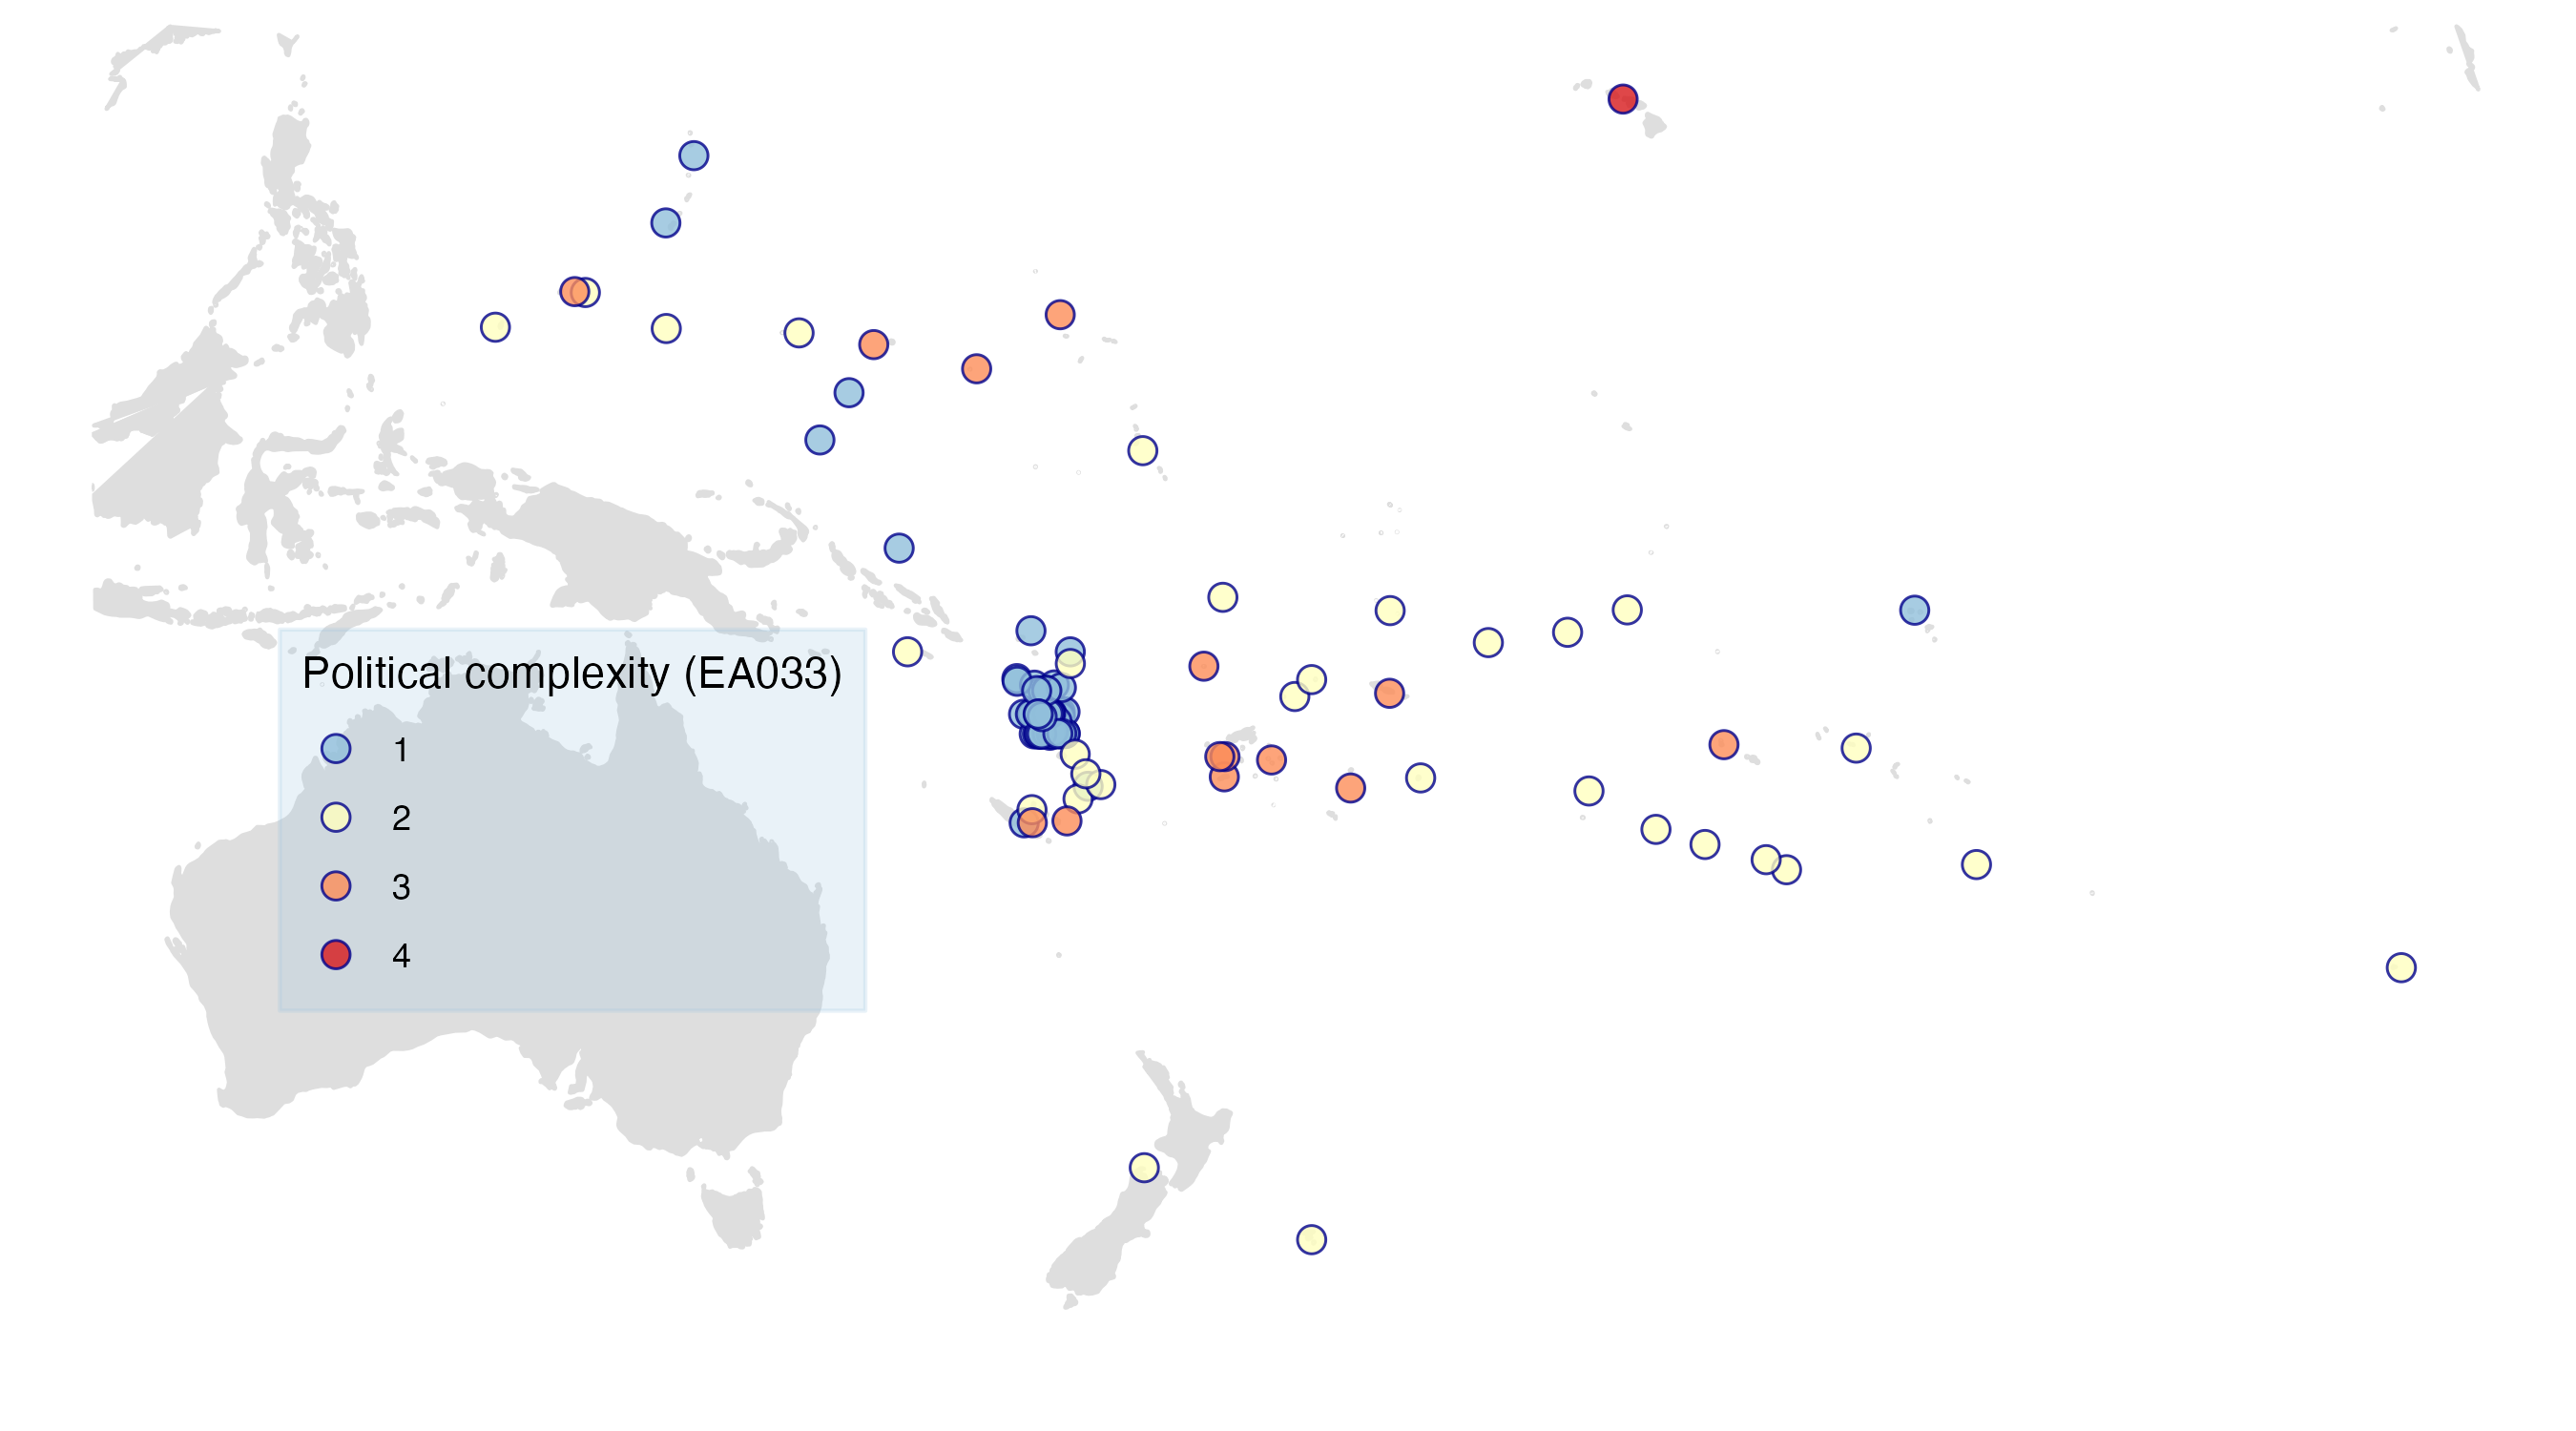
\includegraphics[width=19cm]{map_pol_complex.png}
\caption[Map of Remote Oceania: Political complexity]{{Map of Remote Oceania with associated values for political complexity (EA033).}}
\label{pol_complex_map}
\end{sidewaysfigure}

For the calculations of this study, the mode political complexity per island group was used. 

\FloatBarrier
\subsubsection{Waves of settlement}
\label{appendix_def_dates}
In order to test whether political complexity is driving language diversification in Remote Oceania, we need to control for other relevant variables --- in particular time depth of human settlement. The time of settlement indicates how long a community is likely to have been in a certain place. It can also be a proxy measurement of how similar neighbours are likely to be. If a place has only been inhabited by humans for a short amount of time, then it is likely that the communities that exist there today are not so different from each other. However, in order to take into account similarity between communities fully it is necessary to explicitly include measurements of cultural similarity or phylogenetic distance --- which is not part of the methodology of this study, but is left for future studies.

For most islands in our dataset, there is at least one archaeological study indicating time of first settlement. The archaeological data here is mainly based on an overview of the literature by \citet{rieth_cochrane_2018}, supplemented by the following studies: \citet{intoh2007reconnaissance, intoh2008ongoing, carson2012recent, kirch2012basline, Napolitano_et_al_yap, ellis2012saipan} and \citet{levin_seikel_miles_2019}. 

For most of the island groups, the labels provided in \citet{rieth_cochrane_2018} or the other sources neatly corresponded to the island groups in our data (e.g. Mangareva = Mangareva). However, sometimes the label refers to a larger area, this is the case of ``Austral Islands'' which in our dataset is broken down into Rimatara, Tupuai, Ra'ivavae and Rurutu respectively. In such cases it is assumed that the time can be generalised over the smaller island groups (this is also the case for the political complexity metric). Furthermore, some island groups have not been subject to archaeological research, but they are known to have been settled in association with another place which has been studied. For example, while there have been no archaeological excavations on the Sorol atoll of Micronesia, it is known to be closely related to Ulithi \citep[23]{quackenbush1968sonsorol} and it is likely that it was settled at a similar time. In such cases, the time depth is inferred based on information from nearby islands. For every island, the table in the appendix \ref{dates_table_appendic} lists the label of the island group in the source and if the settlement timing has been inferred based on evidence from nearby islands or not.

Archaeological dates are based on radiocarbon findings which are calibrated based on conditions at the excavation site and other finds there. There exists different calibration methods\footnote{Radiocarbon calibration is the process by which radiocarbon years are converted into calendar years. Because the ratio of atmospheric $^{14}$C/$^{12}$C, which is a key element in this process, has not been stable historically, different methods exist and these may produce different results.}. In order to make the dates from different sites directly comparable they need to be re-calibrated in the same way. It was not possible to access all the necessary information on each publication and re-calibrate the dates appropriately. Instead of using the raw dates from the different studies, the islands have been sorted into a settlement order with twelve waves based on the dates in the literature and descriptions of what was settled in the same wave. Fig.~\ref{dates_map} illustrates the settlement wave order per island. Exact dates and references are found in appendix \ref{dates_table_appendic}.

For comparison across island groups, the oldest settlement order per group was used. Unfortunately, this means that settlement data for Polynesian outliers in Southern Vanuatu, who arrived much more recently, is ignored.

\begin{sidewaysfigure}
\centering
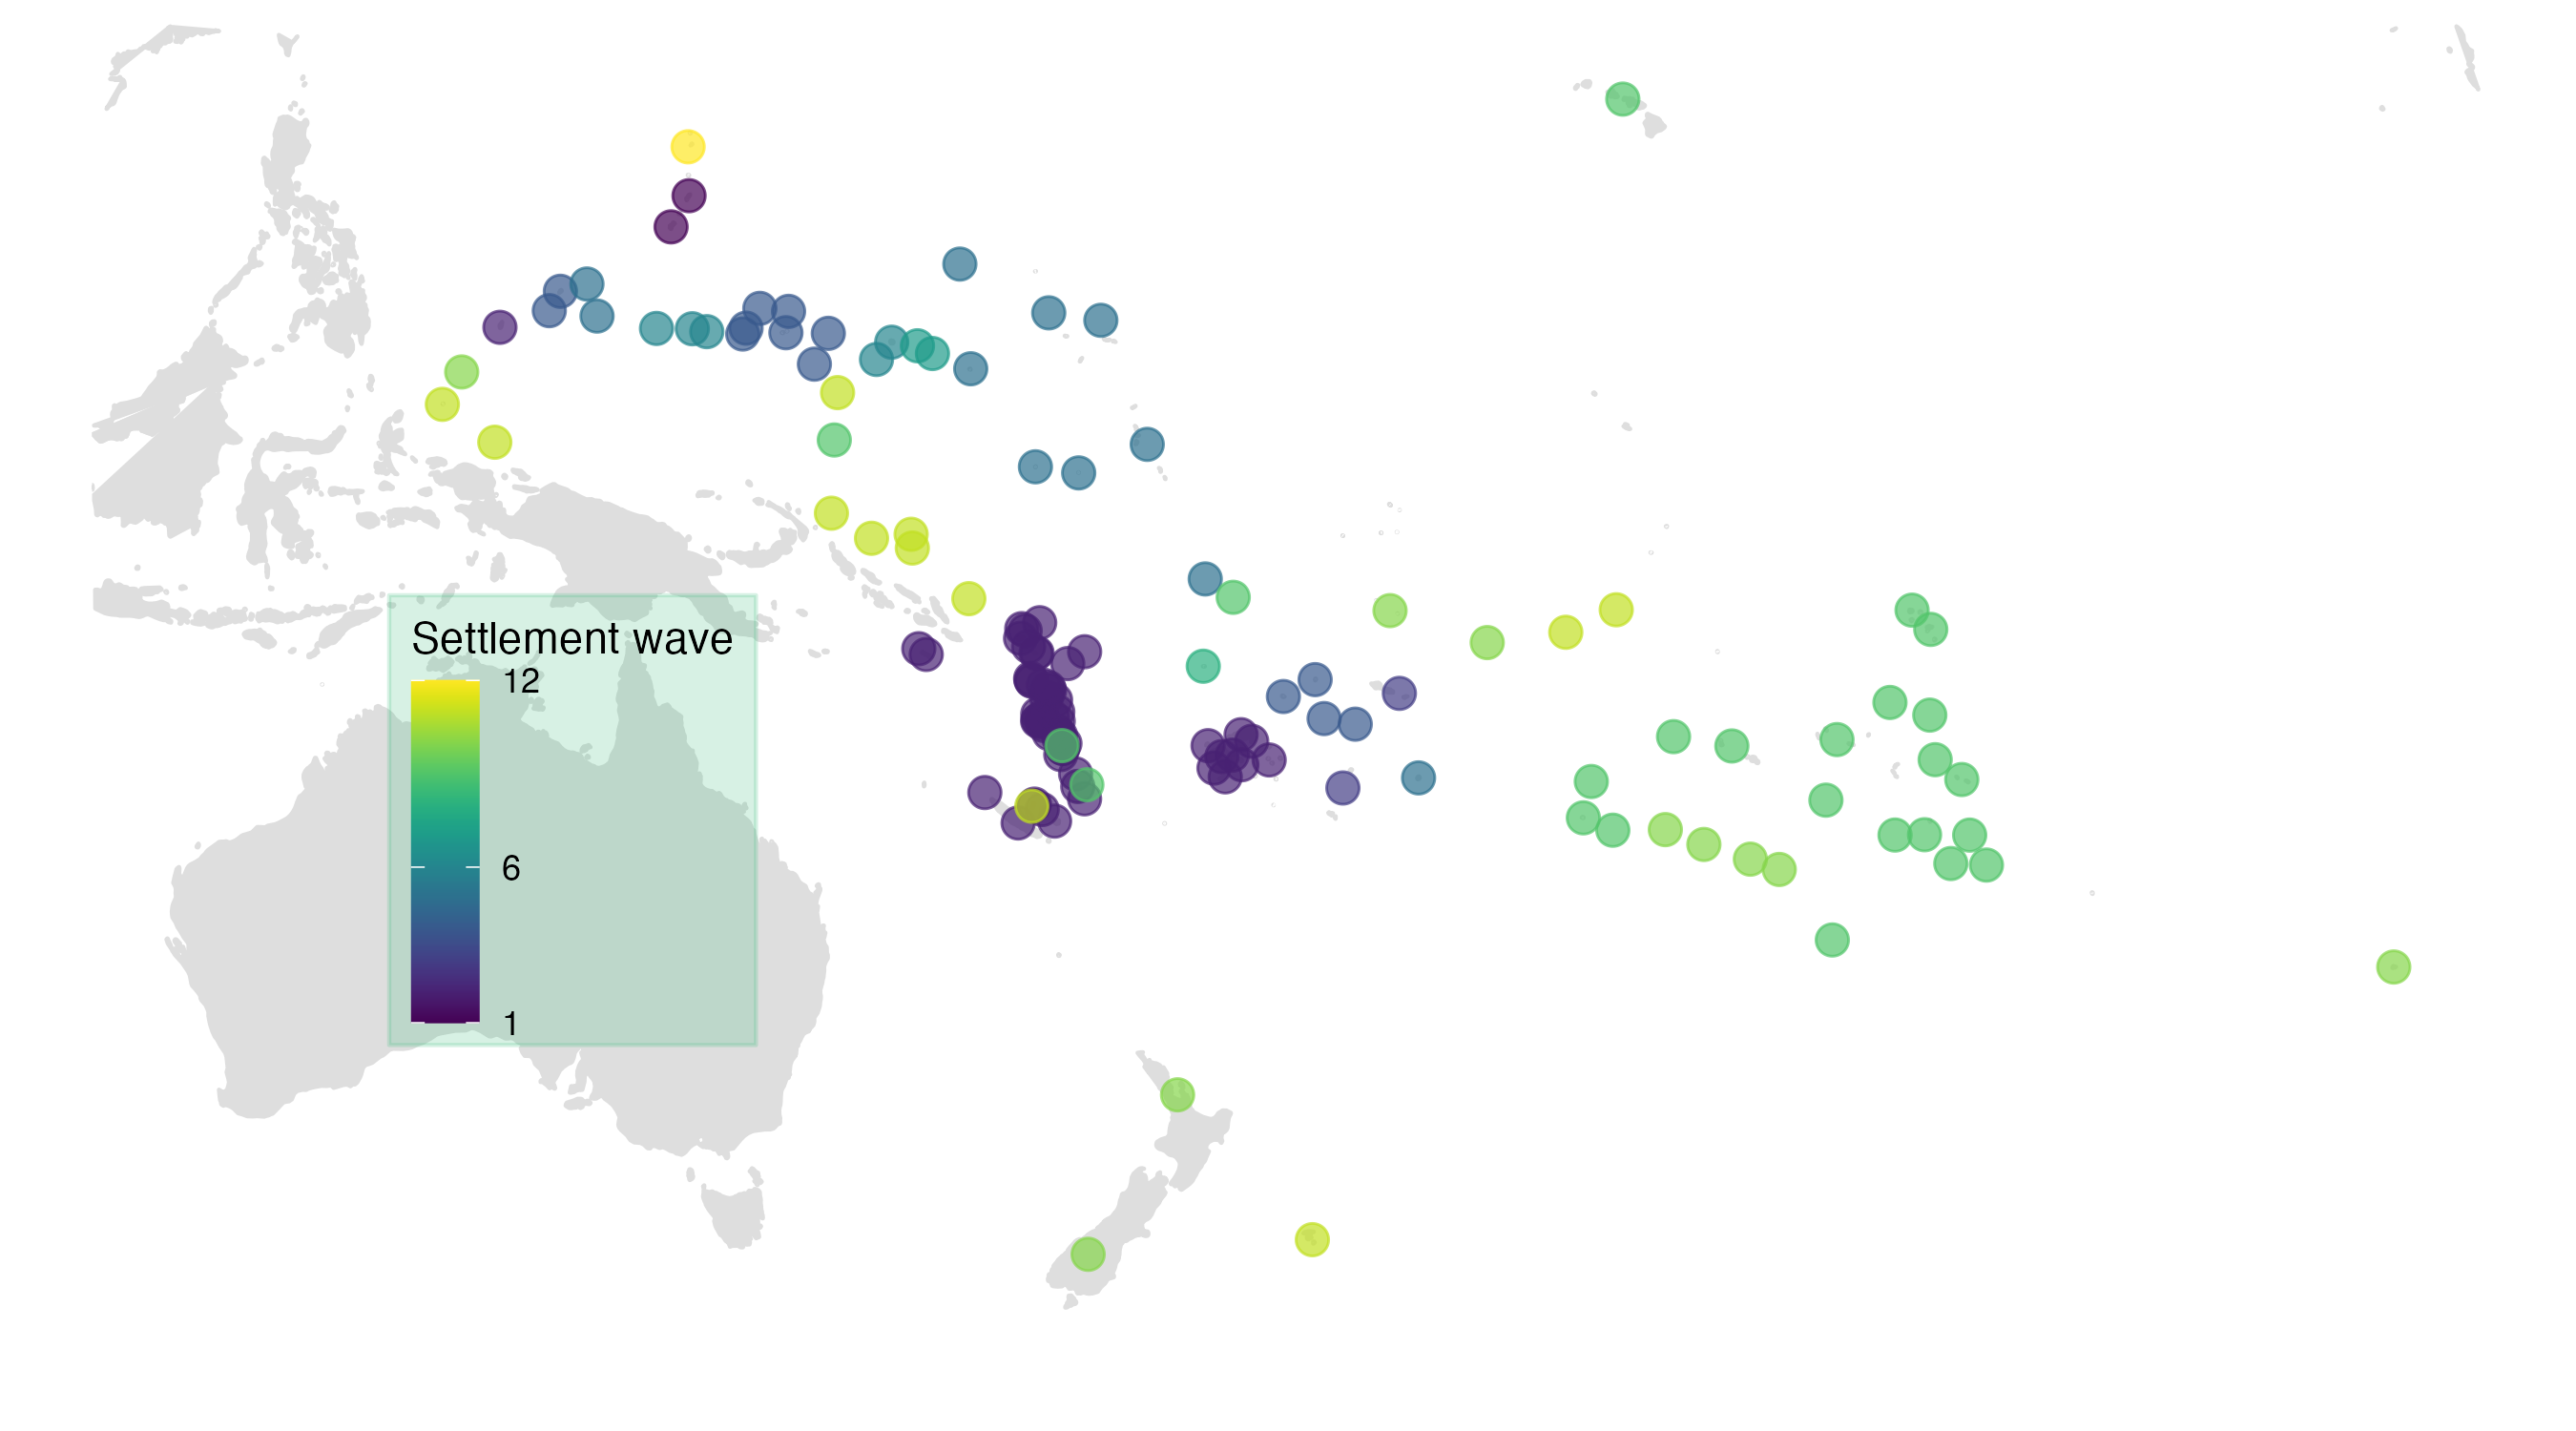
\includegraphics[width=19cm]{Map_RO_dates.png}
\caption{{Map of island groups in Remote Oceania labelled with settlement order.}}
\label{dates_map}
\end{sidewaysfigure}

\FloatBarrier
\subsubsection{Other environmental factors} 
\label{appendix_environ}
As previous studies of language diversification have shown (e.g. \citet{ greenhill2015demographic, gavin2017process, Pacheco_Coelho_2019, hua2019ecological}), environmental factors such as latitude, rainfall etc can be useful in estimating language richness. This is due to the connection between these variables and the ability to sustain several self-sufficient smaller groups.

%In many parts of the world, we have limited data on actual population dynamics --- in particular historically. How many people lived on Efate island 1,000 years ago? This is hard to know. Estimations of carrying capacity can give us an upper limit on how many humans could possible live in an area. The link to languages is as follows: the more groups of people who can sustain themselves on a smaller area each, the more languages there can be in that region.

We are using measurements of absolute latitude, Net Primary Production, Precipitation (rainfall), temperature and size of islands to estimate the environments ability to sustain small groups. The data comes from Global Self-consistent, Hierarchical, High-resolution Geography Database (GSHHG) \citep{wessel1996global}, the ecoClimate database \citep{ecoclimate} and the Moderate Resolution Imaging Spectroradiometer (MODIS, \citet{running2021modis_terra, running2021modis_aqua}). The coordinates of the centroids of each land mass from GSHHG was used to extract the information from ecoClimate and MODIS. The ecoClimate data used are simulations of the pre-industrial period ($\sim$1760).

The Net Primary Production (NPP) data from from MODIS is from 2001, 2002, 2003 and 2004 (these are the oldest available information). NPP reflects the amount of carbon captured by plants in an ecosystem, after accounting for losses due to respiration. The data is gathered by two space satellites (Terra and Aqua) of the United States of America's National Aeronautics and Space Administration (NASA). They collect spectral indices of land-based vegetation, which are then used to infer NPP which is acculmated into a grid where each cell is 500 meters by 500 meters. For more details, see \citet{running2015daily} \footnote{The manual is for a previous release, where the grid cells were 1km by 1km. The more recent release is 500m by 500m.}.

In total, the following environmental variables are included in the study:

\begin{itemize}
\item Global Self-consistent, Hierarchical, High-resolution Geography Database (GSHHG)
\begin{itemize}
    \item Absolute latitude
    \item Shoreline
\end{itemize}
\item ecoClimate
\begin{itemize}
\item Bio1: Annual mean temperature (Celsius)
\item Bio4: Temperature seasonality (standard deviation *100)
\item Bio12: Annual precipitation (mm/m2)
\item Bio15: Precipitation seasonality (coefficient of variation)
\end{itemize}
\item Moderate Resolution Imaging Spectroradiometer (MODIS)
\begin{itemize}
    \item MOD17A3HGF.061: NPP data from the satellite Terra
    \item MYD17A3HGF.061: NPP data from the satellite Aqua
\end{itemize}
\end{itemize}

%number_of_languages_vs_pop_1950_log10.png
%number_of_languages_vs_pop_1950.png

\FloatBarrier

\newpage
\subsubsection{PCA of environmental variables}
\label{appendix_eniron_PCA}


\newpage
\subsection{Caveat regarding time-span}
\label{appendix_time_span}
%Collected thoughts in regards to validity of ethnographic data, may be cut.

To understand the vast majority of human history and diversification, we should consider the state of societies as they were before the introduction of Western colonisation, industrialisation, globalization etc as these have only been around in the last 500 years. Behaviourally modern humans emerged between 90,000 and 160,000 years ago (\citet{powell2009late}: \cite{marean2007early}). The last 500 years represent between 0.6\% and 0.3\% of our history. If we consider only the time period of more sedentary living and agriculture, i.e. approx the last 11,000 years (c.f. \citet{kislev2006early}) the proportion of time since Columbus landing in the Caribbean is 4.5\%.

The aforementioned processes, while recent, have resulted in mass immigration/invasion (c.f. \citet{invasion_day}) to places like the Americas, South Africa, Australia and New Zealand and oppressive policies that reduce language diversity. They have had a massive impact in the comparatively short time span that they have been active and are not only perpetuated by Western forces but also other powerful groups (see for example the case of Indonesian power in Western New Guinea \citep{gietzelt1989indonesianization}). Another driving force that is relatively recent and related is the emergence of modern nation-states (c.f. \citet{foucault2007security}, \citet[21-22]{oakes2001language}). In connection with the aforementioned forces, the formation of modern nation-states has further reduced diversity that was present within groups (through means like ideological movements (e.g.the \emph{Volkgeist}-movement), nationally standardized mass education, mass media, print-media etc). The creation of nation-states and their continued development is tied to ideas of one sole homogeneous culture (c.f. \citet{encyclo_nationalism}), which often results in the disappearance of regional variation, minority languages etc within what we today conceive of as ``countries''/``nation-states''. 

The massive effect of these forces in the last 500 years means that as a historical scientist, there is a big difference between considering the human landscape before and after this point --- especially in terms of cultural history and diversity. \citet[7340-7341]{curriemace2009} find that the data available for language territories in Australia and the Americas is so affected by colonial history and population replacement to make it impossible to include it in the analysis alongside the other regions. 

There is also a problem with data pertaining to history before these massive forces step onto the stage. Ethnographic accounts are often ``snapshots'' with unclear time-depth 
 \citep[113]{bedford2008northern}. Human culture everywhere is dynamic and changing. This is one of the reasons why the ethnographic database D-PLACE \citep{d_place_all} includes ``focal year'' for each variable.




\newpage
\subsection{Regarding population and the number of languages}
\label{appendix_pop_vs_languages}
While it is true that the number of languages is not entirely evenly spread out over the population, it is still the case that there is a general trend connecting a greater number of people with a greater number of languages (as can be seen in Figs \ref{fig:un_pop_plot} and \ref{fig:un_pop_plot_log10}). However, due to difficulties with data, this is hard to study historically. In this particular study, population numbers could not be included due to a lack of detailed and reliable enough data on enough island groups prior to Western colonization. While resources like \citet{elcat} have population numbers for many places, it does not sufficiently cover Oceania to allow the variable to be included. This is similar to \citet[7340-7341]{curriemace2009} who found that the data available for language territories in Australia and the Americas is so affected by colonial history and population replacement to make it impossible to include it in the analysis alongside the other regions. 

Figs \ref{fig:un_pop_plot} and \ref{fig:un_pop_plot_log10} show the relationship between the number of languages per modern country/territory \citep{glottolog4_5} and its population in 1950 \citep{UN_pop}, with Remote Oceanic countries and territories highlighted. Modern nation-states are not historically relevant cultural units in many places in the world, include the Pacific. For example, Cook Islands (also known as Avaiki Nui) and the Federated States of Micronesia encompasses many island groups with diverse histories (c.f. Fig \ref{RO_overnight_coloured_dots} and Appendix \ref{sec:island_geo}). However, even with this noise, there is a relationship --- more people $\rightarrow$ more languages.

\begin{figure}[ht]
    \centering
    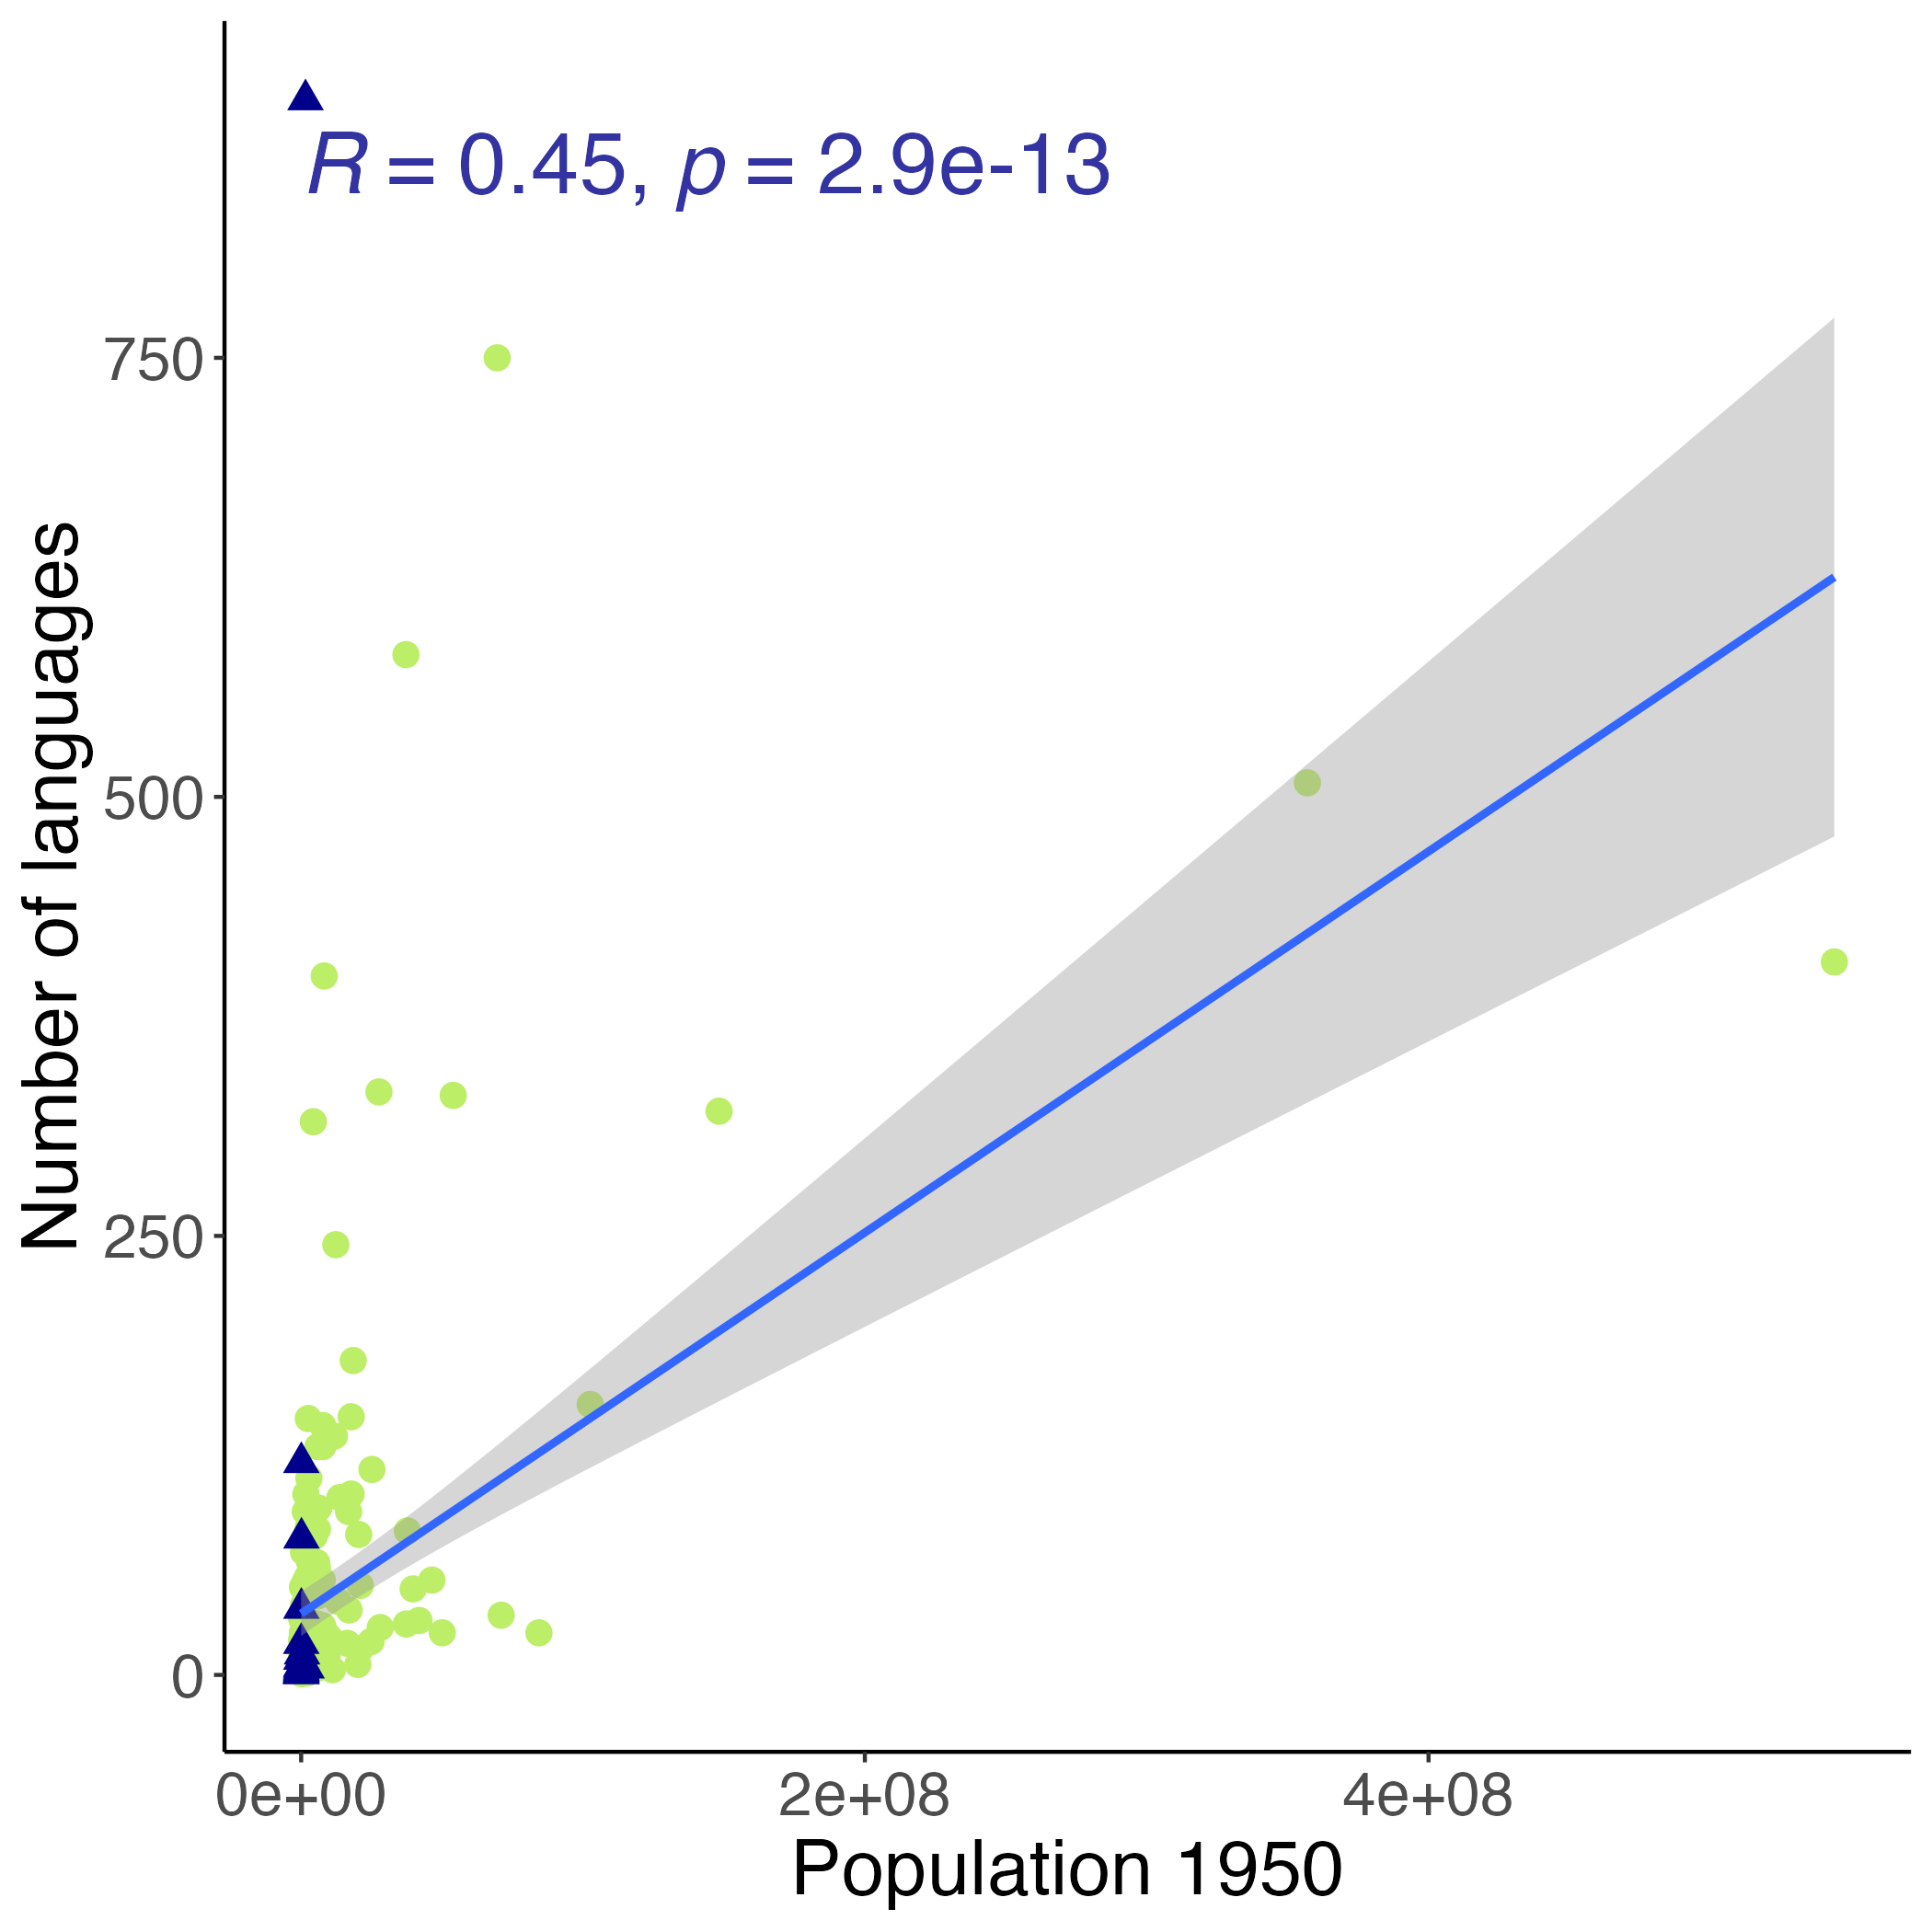
\includegraphics[width=.8\linewidth]{number_of_languages_vs_pop_1950.png}
    \caption{Population in 1950 per country (x-axis) and number of languages per country (y-axis). Dark blue triangles = countries with at least some landmasses in Remote Oceania, green circles = all other countries.}
        \label{fig:un_pop_plot}
    \end{figure}
\begin{figure}[ht]
    \centering
          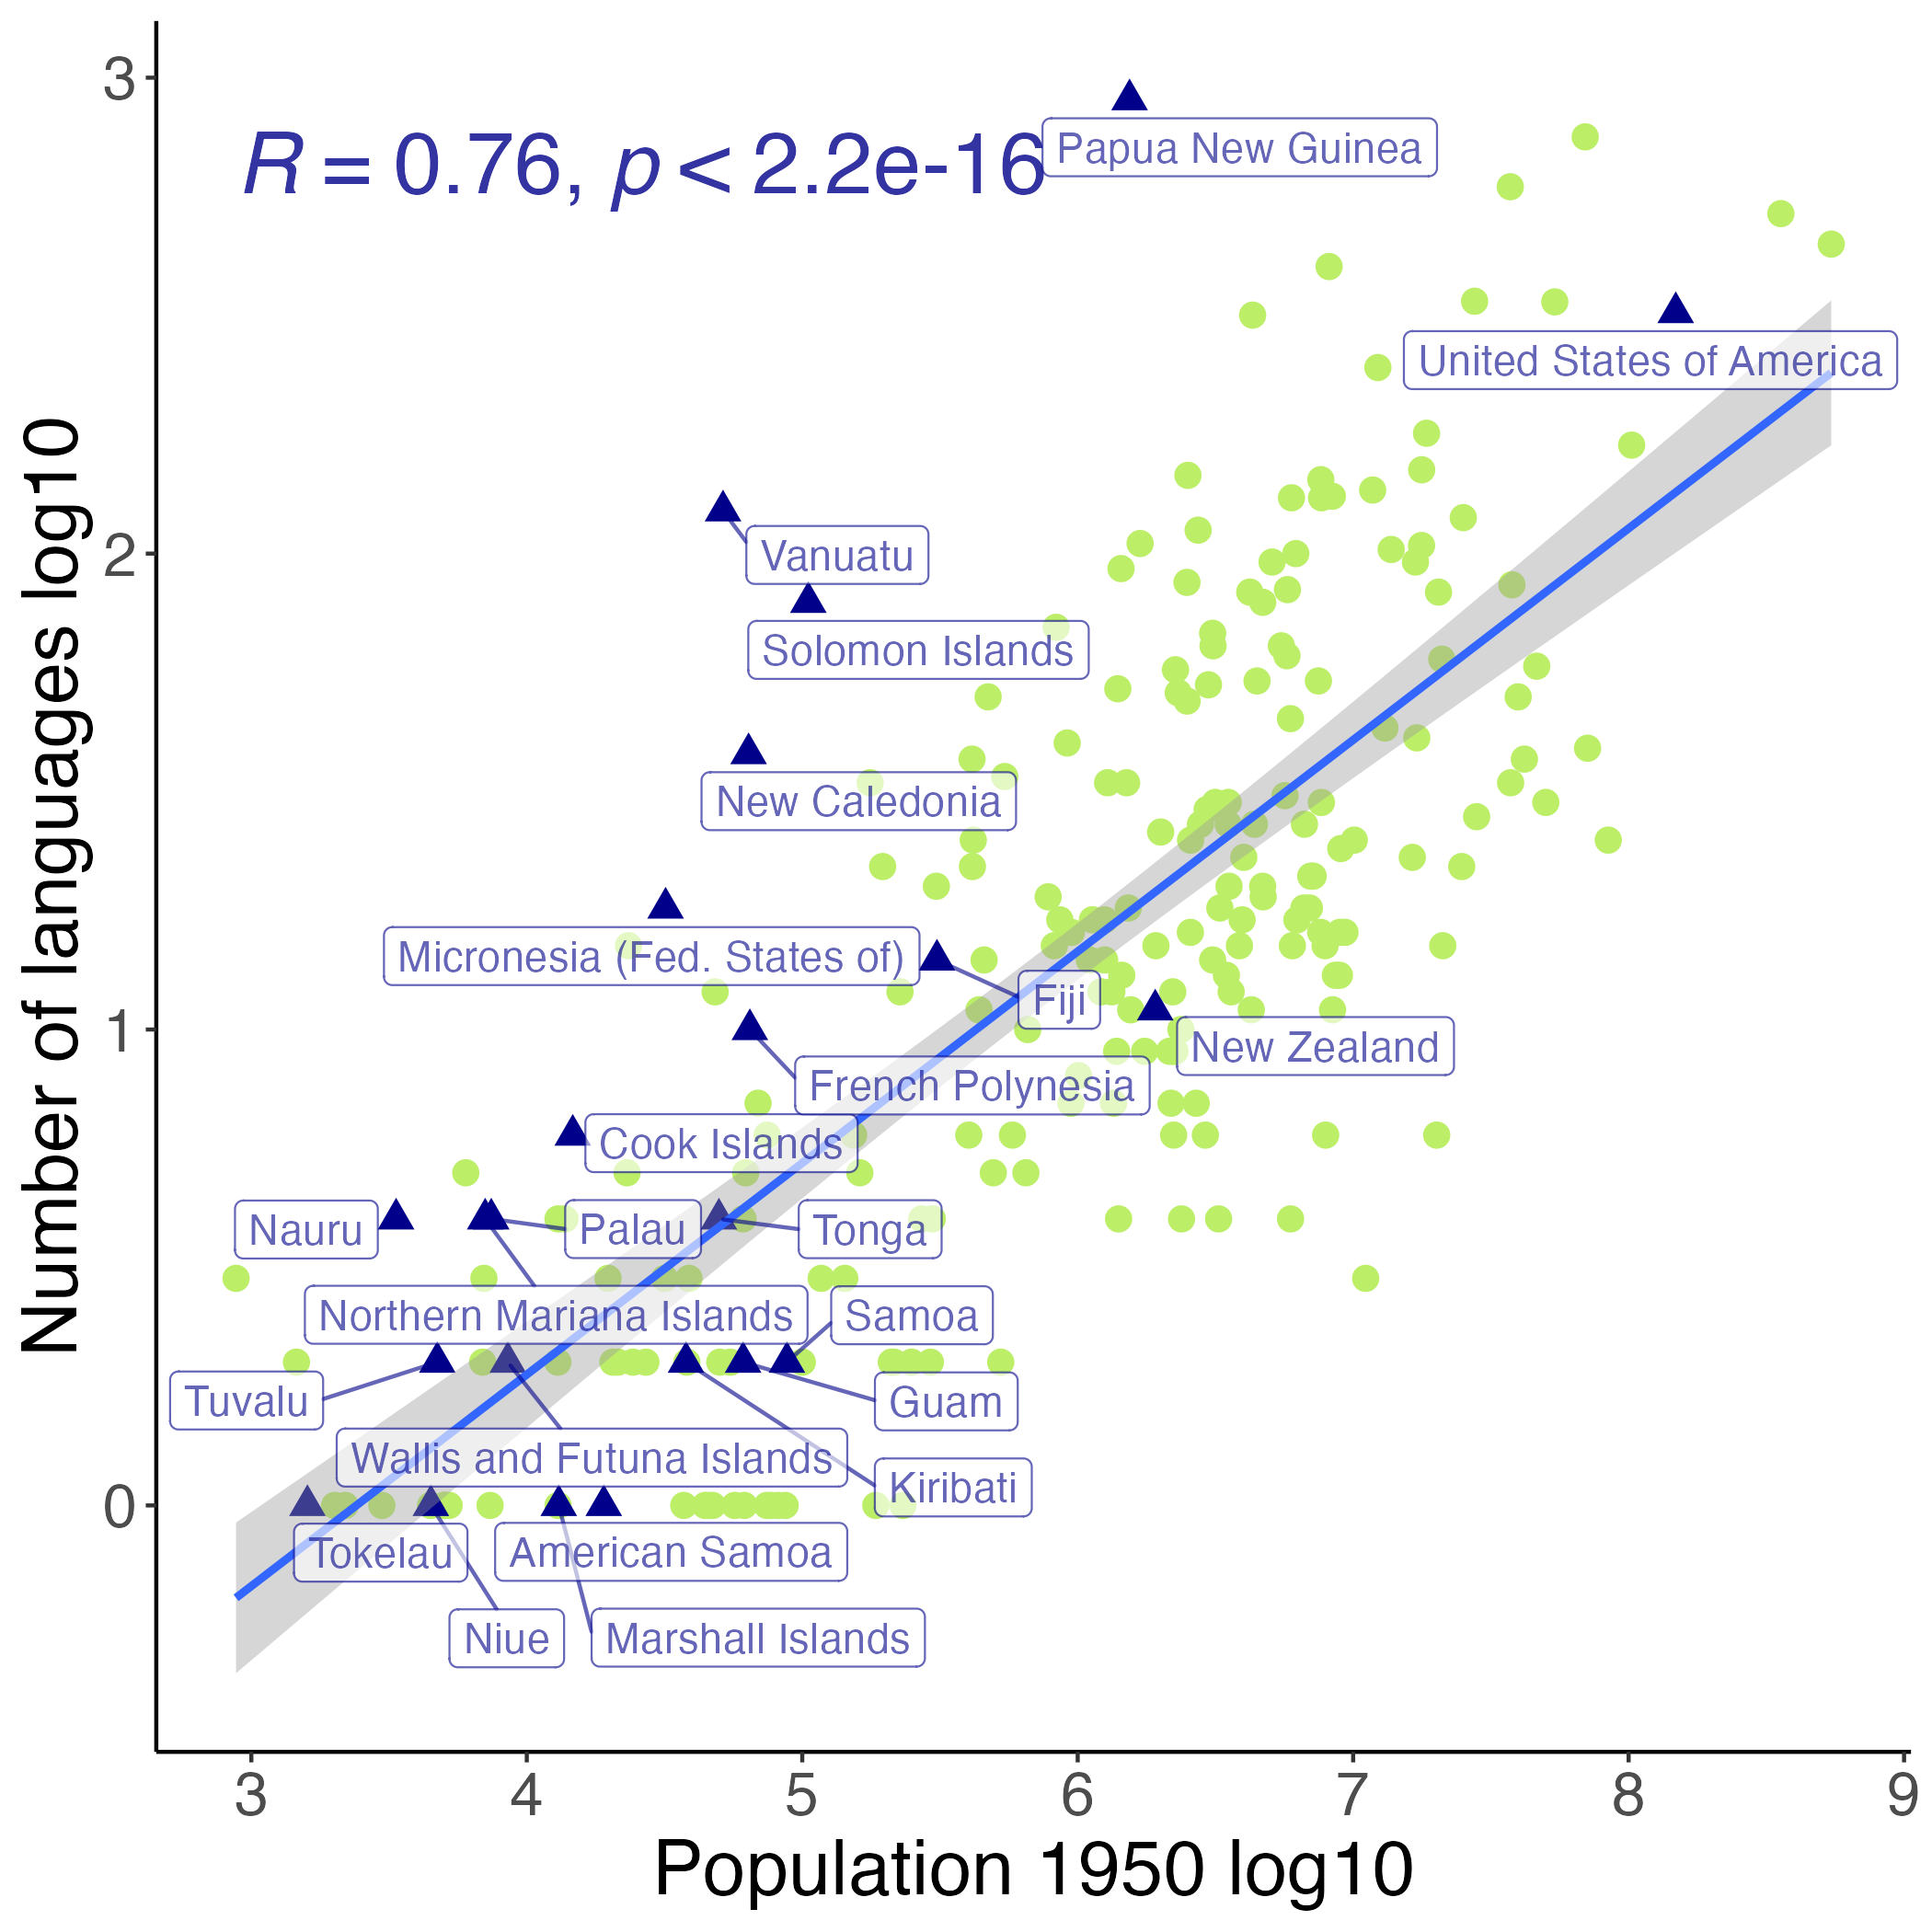
\includegraphics[width=.8\linewidth]{number_of_languages_vs_pop_1950_log10.png}
    \caption{Population in 1950 per country (x-axis) and number of languages per country (y-axis) - log-10-transformed. Dark blue triangles = countries with at least some landmasses in Remote Oceania, green circles = all other countries.}
    \label{fig:un_pop_plot_log10}
    \end{figure}

While it is not possible to include population size as a variable, it is possible that the environmental variables are relevant here as they may suggest island groups that could be home to larger populations. Fig. \ref{SPLOM_country_all_variables} shows the relationship between the population data and language count data above to the variables of this study. The first four rows represent the data summarised per entire countries  (i.e. from  \citet{UN_pop} and \citet{glottolog4_5}) and the rest are per island group in Remote Oceania. This means there is a mismatch of units of analysis, for example: Hawai'i is a part of the United States of America and therefore is included in the data point for the entire USA. The ``lg count (island group)'' contains only the number of languages in Hawai'i in the island groups included in this study, i.e. 1.

\begin{figure}[ht]
    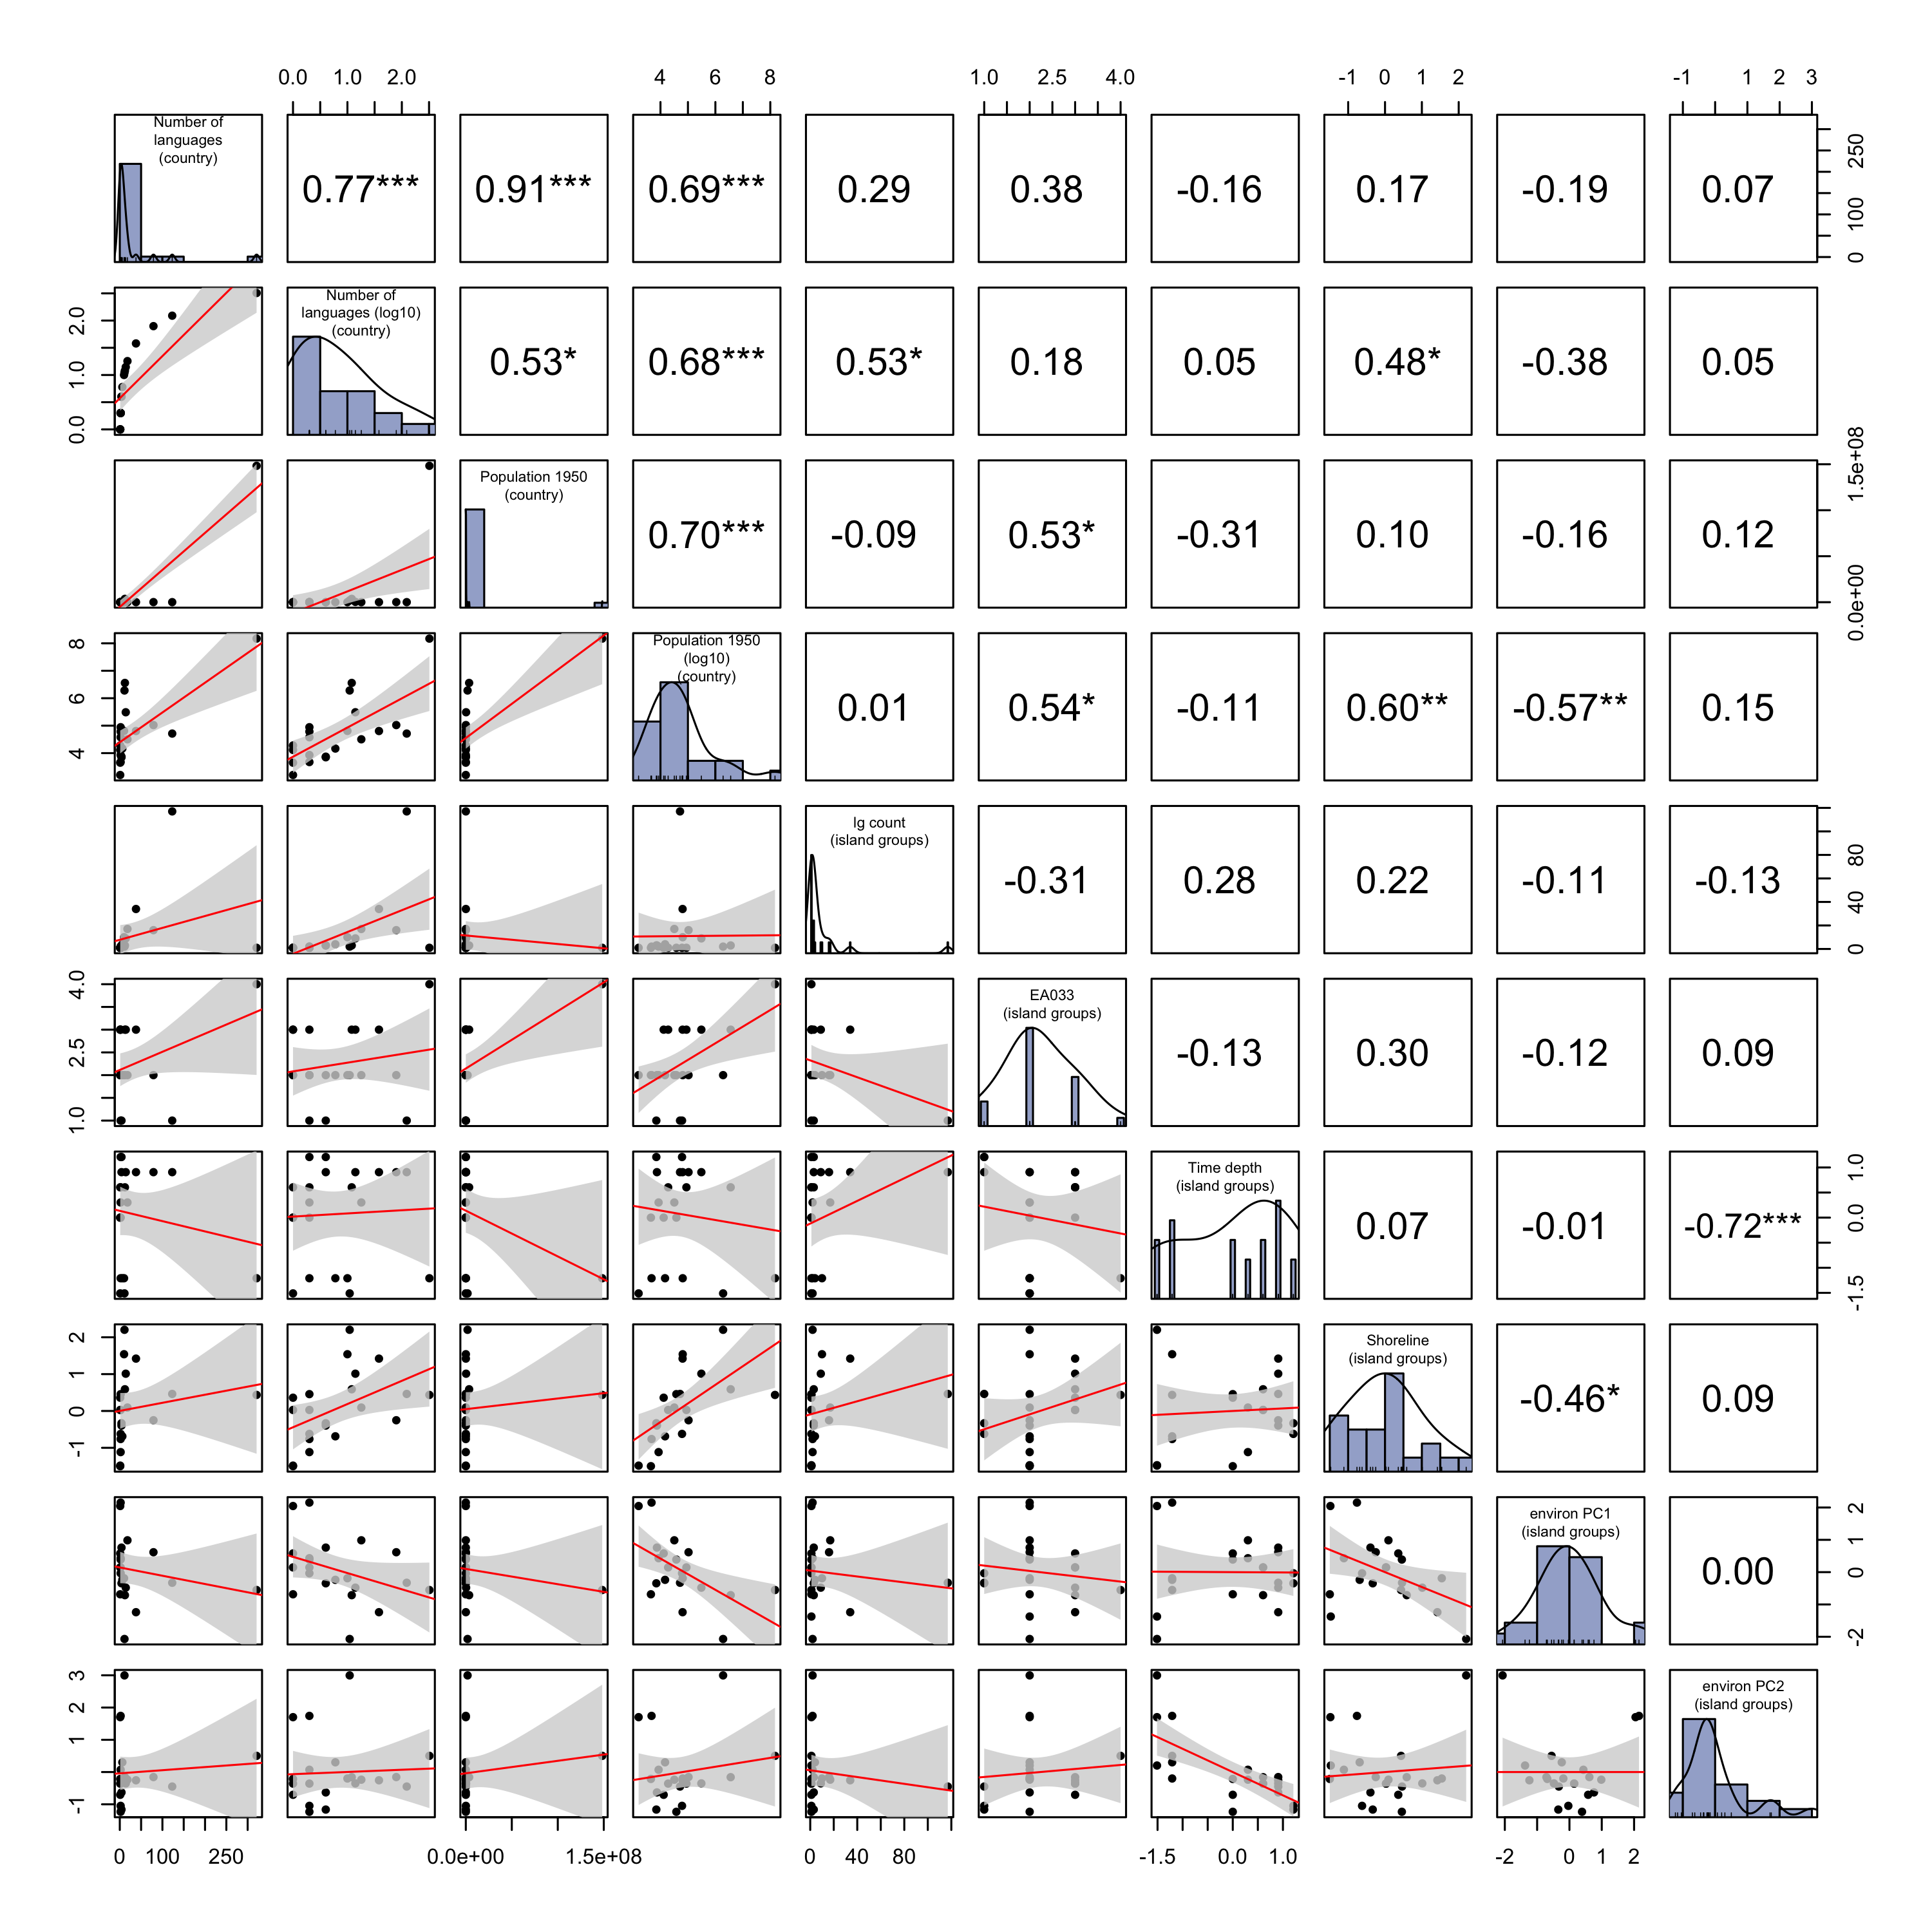
\includegraphics[width=15cm]{latex/SPLOM_country_all_variables.png}
\caption{Scatterplot matrix of all variables available, over countries. Note that the population data is taken from \citet{UN_pop} and refers to the whole country, i.e. the population of the entire USA --- not just Hawai'i..}
\label{SPLOM_country_all_variables}
\end{figure}


There is a negative correlation of -0.56 between the population (log10) per country and the environmental PC1 per island group. This may indicate that the environmental PCs are picking up on information relevant to population size.

\FloatBarrier
\newpage
\subsection{Table of political complexity per island group }
\singlespacing
\label{appendix_pol_complex}

% latex table generated in R 4.4.2 by xtable 1.8-4 package
% Tue Nov 26 22:11:05 2024
\begin{longtable}{p{4.5cm}p{2cm}p{2cm}p{4cm}p{4cm}}
  \toprule
Island group (overnight-sailing) & Island group (shared language) & Political complexity (EA033) & glottocodes & References \\ 
  \midrule
Aotearoa & Aotearoa & 2 & maor1246 & \citet{sahlins1958social}, \citet{buck1952}, \citet{kirch1984evolution}, \citet{van1995maori} \\ 
  Banaba & Tungaru + Tuvalu & 2 & gilb1244 & \citet{lambert1966}, \citet{lambert1975makin}, \citet{lambert1991}, \citet{macdonald1982cinderellas} \\ 
  Chuuk & Chuuk & 2 & chuu1238 & \citet{goodenough1991}, \citet{goodenough2002under}, \citet{mahony1960taro} \\ 
  East Futuna & East Futuna & 2 & east2447 & \citet{kirch1994wet} \\ 
  Fiji & Kadavu & 3 & kada1285 & \citet{kuhlken2002intensive}, \citet{scarr1984fiji}, \citet{walter1978examination} \\ 
  Fiji & Lau & 3 & laua1243 & \citet{hocart_1929}, \citet{quain_1948}, \citet{thompson1940a}, \citet{thompson1940b} \\ 
  Fiji & Viti Levu + Yasawa & 3 & sout2864, nort2843 & \citet{kuhlken2002intensive}, \citet{scarr1984fiji}, \citet{walter1978examination} \\ 
  Hawaii & Hawaii & 4 & hawa1245 & \citet{kirch1994wet}, \citet{kirch2010chiefs} \\ 
  Hereheretue & Tuamotu & 2 & tuam1242 & \citet{emory1975material} \\ 
  Kanaky (main island + Loyalties) & Kanaky (New Caledonia main island) & 1 & ajie1238 & \citet{winslow1991} \\ 
  Kanaky (main island + Loyalties) & Kanaky (New Caledonia main island) & 3 & xara1244 & \citet{young1991goodenough} \\ 
  Kanaky (main island + Loyalties) & Lifou & 2 & dehu1237 & \citet{hadfield_1920}, \citet{ray1917people} \\ 
  Kanaky (main island + Loyalties) & Nengone & 3 & neng1238 & \citet{dubois1984gens}, \citet{guiart1952organisation} \\ 
  Kapingamarangi & Kapingamarangi & 1 & kapi1249 & \citet{buck1950} \\ 
  Kosrae & Kosrae & 3 & kosr1238 & \citet{athens2007prehistoric}, \citet{graves1986late}, \citet{peoples1991} \\ 
  Laguas yan gåni (Guam + Northern Marianas) & Laguas yan gåni (Guam + Northern Marianas) & 1 & cham1312, caro1242 & \citet{cordy1983social}, \citet{thompson_1971}, \citet{josephandmurray1951}, \citet{spehr1954} \\ 
  Luangiua + Nukumanu & Luangiua & 1 & onto1237 & \citet{sahlins1958social}, \citet{bayliss1974constraints}, \citet{donner1991} \\ 
  Mangaia & Avaiki Nui (south) & 2 & raro1241 & \citet{bellwood1971varieties}, \citet{buck1934}, \citet{crocombe_1967}, \citet{hayes1981cook}, \citet{walter1996} \\ 
  Mangareva & Mangareva & 2 & mang1401 & \citet{buck1938}, \citet{conte2004archaeological}, \citet{green2000mangarevan} \\ 
  Marquesas & Te Henua ‘Enana (North Marquesas) & 1 & nort2845 & \citet{sahlins1958social} \\ 
  Marutea & Tuamotu & 2 & tuam1242 & \citet{emory1975material} \\ 
  Mo-ava-mo-iki (Bellona + Rennelle) & Mo-ava-mo-iki (Bellona + Rennelle) & 2 & renn1242 & \citet{birketsmith1956}, \citet{monberg1991bellona} \\ 
  Morane & Tuamotu & 2 & tuam1242 & \citet{emory1975material} \\ 
  Māngarongaro & Māngarongaro & 2 & penr1237 & \citet{buck1932b} \\ 
  Napuka & Tuamotu & 2 & tuam1242 & \citet{emory1975material} \\ 
  Ngatik & Pohnpei & 3 & pohn1238 & \citet{hanlon2019upon}, \citet{haun1984prehistoric}, \citet{raynor1991indigenous}, \citet{riesenberg1968native} \\ 
  Ngā Pū Toru & Avaiki Nui (south) & 2 & raro1241 & \citet{bellwood1971varieties}, \citet{buck1934}, \citet{crocombe_1967}, \citet{hayes1981cook}, \citet{walter1996} \\ 
  Niu + Tuvalu & Tungaru + Tuvalu & 2 & gilb1244, tuva1244 & \citet{lambert1966}, \citet{lambert1975makin}, \citet{lambert1991}, \citet{macdonald1982cinderellas}, \citet{goldsmith1991} \\ 
  Niue & Niue & 2 & niue1239 & \citet{loeb1978}, \citet{smith1983niue}, \citet{walter_anderson1995} \\ 
  Nukuoro & Nukuoro & 1 & nuku1260 & \citet{carroll1966nukuoro}, \citet{carroll1975pacific}, \citet{eilers_1934} \\ 
  Nukutaveke 59 & Tuamotu & 2 & tuam1242 & \citet{emory1975material} \\ 
  Nukutaveke 61 & Tuamotu & 2 & tuam1242 & \citet{emory1975material} \\ 
  Palau & Palau & 2 & pala1344 & \citet{force1960leadership} \\ 
  Pohnpei & Pohnpei & 3 & pohn1238 & \citet{hanlon2019upon}, \citet{haun1984prehistoric}, \citet{raynor1991indigenous}, \citet{riesenberg1968native} \\ 
  Pukapuka & Pukapuka & 2 & puka1242 & \citet{beagleholeandbeaglehole1938}, \citet{macgregor1935} \\ 
  Raivavae & Raivavae & 2 & raiv1237 & \citet{aitken1930ethnology}, \citet{bollt2008excavations}, \citet{edwards2003archaeological} \\ 
  Rakahanga-Manihiki & Rakahanga-Manihiki & 2 & raka1237 & \citet{buck1932a} \\ 
  Rapa Nui & Rapa Nui & 2 & rapa1244 & \citet{sahlins1958social}, \citet{kirch1984evolution}, \citet{metraux_1971} \\ 
  Raro Matai + Nia Matai & Tahiti & 3 & tahi1242 & \citet{oliver2019ancient} \\ 
  Rarotonga & Avaiki Nui (south) & 2 & raro1241 & \citet{bellwood1971varieties}, \citet{buck1934}, \citet{crocombe_1967}, \citet{hayes1981cook}, \citet{walter1996} \\ 
  Ratak + Rālik & Ratak + Rālik & 3 & mars1254 & \citet{carruci1991marshall}, \citet{erdland1914}, \citet{williamson_1982} \\ 
  Rotuma & Rotuma & 3 & rotu1241 & \citet{gardiner1898natives}, \citet{howard1963conservatism}, \citet{howard1991} \\ 
  Rurutu & Rurutu & 2 & ruru1237 & \citet{aitken1930ethnology}, \citet{bollt2008excavations}, \citet{edwards2003archaeological} \\ 
  Rēkohou & Rēkohou & 2 & mori1267 & \citet{sahlins1958social}, \citet{buck1952}, \citet{kirch1984evolution}, \citet{van1995maori} \\ 
  Sorol & Ulithi (greater) & 2 & ulit1238 & \citet{lessa1950}, \citet{lessa1966} \\ 
  Sāmoa & Sāmoa & 3 & samo1305 & \citet{sahlins1958social}, \citet{buck1930}, \citet{keesing1934}, \citet{watters_1958} \\ 
  Tatakoto + Reao & Tuamotu & 2 & tuam1242 & \citet{emory1975material} \\ 
  Tokelau & Tokelau & 2 & toke1240 & \citet{hooper1973demographic}, \citet{macgregor1937} \\ 
  Tonga & Tonga & 3 & tong1325 & \citet{kirch1984evolution}, \citet{cummins1977tongan}, \citet{ferdon1988early} \\ 
  Tuamotu + Puka-puka & Tuamotu & 2 & tuam1242 & \citet{emory1975material} \\ 
  Tungaru & Tungaru + Tuvalu & 2 & gilb1244 & \citet{lambert1966}, \citet{lambert1975makin}, \citet{lambert1991}, \citet{macdonald1982cinderellas} \\ 
  Tupuai & Tupuai & 2 & tubu1240 & \citet{aitken1930ethnology}, \citet{bollt2008excavations}, \citet{edwards2003archaeological} \\ 
  Tureia & Tuamotu & 2 & tuam1242 & \citet{emory1975material} \\ 
  Tuvalu 31 & Tungaru + Tuvalu & 2 & tuva1244 & \citet{macdonald1982cinderellas}, \citet{goldsmith1991} \\ 
  Tuvalu 32 & Tungaru + Tuvalu & 2 & tuva1244 & \citet{macdonald1982cinderellas}, \citet{goldsmith1991} \\ 
  Ulithi + Yap & Ulithi (greater) & 2 & ulit1238 & \citet{lessa1950}, \citet{lessa1966} \\ 
  Ulithi + Yap & Yap & 3 & yape1248 & \citet{huntetal1949}, \citet{muller1917}, \citet{murdocketal1944b}, \citet{salesius1906}, \citet{schneider1953}, \citet{schneider1957_yap}, \citet{schneider1962}, \citet{tetens_savages}, \citet{tetensandkubary1873} \\ 
  Uvea (Wallis) & Uvea (Wallis) & 2 & wall1257 & \citet{burrows1937}, \citet{pollock1995power} \\ 
  Vanuatu + Temotu & Ambae & 1 & east2443, west2513 & \citet{bonnemaison1972systeme} \\ 
  Vanuatu + Temotu & Ambrym & 1 & sout2859 & \citet{tonkinson1981church} \\ 
  Vanuatu + Temotu & Aneityum & 2 & anei1239 & \citet{humphreys1926}, \citet{spriggs1982taro}, \citet{spriggs1986landscape} \\ 
  Vanuatu + Temotu & Anuta & 1 & anut1237 & \citet{feinberg1988socio}, \citet{feinberg1991}, \citet{kirch2002te} \\ 
  Vanuatu + Temotu & Aore & 1 & aore1237 & \citet{bonnemaison1996power} \\ 
  Vanuatu + Temotu & Duff + Reef Islands & 1 & ayiw1239 & \citet{davenport1969} \\ 
  Vanuatu + Temotu & Efate & 2 & nort2836 & \citet{facey1981hereditary} \\ 
  Vanuatu + Temotu & Erromango & 2 & siee1239 & \citet{humphreys1926}, \citet{spriggs1989archaeological} \\ 
  Vanuatu + Temotu & Futuna + Aniwa & 2 & futu1245 & \citet{capell1958culture} \\ 
  Vanuatu + Temotu & Hiu & 1 & hiww1237 & \citet{bonnemaison1996power} \\ 
  Vanuatu + Temotu & Loh-Toga & 1 & loto1240 & \citet{bonnemaison1996power} \\ 
  Vanuatu + Temotu & Maewo & 1 & baet1237, cent2058, mari1426 & \citet{bonnemaison1996power} \\ 
  Vanuatu + Temotu & Malakula & 1 & aulu1238, avok1244, axam1237, bign1238, burm1263, bwen1239, dixo1238, katb1237, labo1244, lare1249, lete1241, ling1265, litz1237, maee1241, malf1237, malu1245, mara1399, mask1242, mpot1241, nese1235, nisv1234, niti1249, port1285, rere1240, unua1237, urip1239, vinm1237, vivt1234, sout2857 & \citet{bonnemaison1996power}, \citet{deacon1934} \\ 
  Vanuatu + Temotu & Mota & 1 & mota1237 & \citet{bonnemaison1996power} \\ 
  Vanuatu + Temotu & Mota Lava & 1 & motl1237 & \citet{bonnemaison1996power} \\ 
  Vanuatu + Temotu & Paama & 1 & paam1238 & \citet{bonnemaison1996power} \\ 
  Vanuatu + Temotu & Pentecost & 1 & saaa1241 & \citet{lane1956} \\ 
  Vanuatu + Temotu & Santo & 1 & butm1237, polo1242, akei1237, ambl1237, fort1240, lore1244, mere1242, moro1286, noku1237, piam1242, rori1237, saka1289, shar1244, tamb1253, tasm1246, tial1239, tolo1255, valp1237, wail1242, wusi1237, tang1347 & \citet{bonnemaison1996power} \\ 
  Vanuatu + Temotu & Tanna & 1 & sout2869 & \citet{lindstroem1991} \\ 
  Vanuatu + Temotu & Tikopia & 2 & tiko1237 & \citet{kirch1994wet}, \citet{sahlins1958social}, \citet{firth1939primitive}, \citet{firth1959social}, \citet{firth1991} \\ 
  Vanuatu + Temotu & Ureparapara & 1 & leha1243, leha1244 & \citet{bonnemaison1996power} \\ 
  Vanuatu + Temotu & Vanua Lava & 1 & leme1238, vera1241, vure1239 & \citet{bonnemaison1996power} \\ 
  Woleai & Woleai & 2 & wole1240 & \citet{alkire1991woleai}, \citet{burrowsandspiro1953} \\ 
  Ānewetak & Ratak + Rālik & 3 & mars1254 & \citet{carruci1991marshall}, \citet{erdland1914}, \citet{williamson_1982} \\ 
   \bottomrule
\caption{Table of political complexity values (EA033).} 
\label{appendix_pol_complex_xtable}
\end{longtable}


\newpage
\subsection{Table of settlement date per island group based on archaeology}
\singlespacing
\label{dates_table_appendic}

\FloatBarrier
\newpage
\subsection{Input data tables}
\singlespacing
\label{appendix_data tables}

% latex table generated in R 4.3.1 by xtable 1.8-4 package
% Fri Aug 25 17:55:22 2023
\begin{longtable}{p{4.5cm}p{1.4cm}p{1.4cm}p{1.4cm}p{1.4cm}p{1.7cm}p{1.7cm}p{1.7cm}}
  \toprule
Island group (shared language) & Lang count & Shoreline & environ PC1 & environ PC2 & environ PC3 & Political complexity (EA033) & Time depth \\ 
  \midrule
Malakula & 33 & 1.010 & -0.612 & -0.836 & -0.662 & -1.110 & 0.864 \\ 
  Kanaky (New Caledonia main island) & 29 & 2.275 & -1.420 & -0.254 & -1.210 & -1.110 & 0.864 \\ 
  Santo & 24 & 1.038 & -0.340 & -0.853 & -0.347 & -1.110 & 0.864 \\ 
  Ambrym & 6 & -0.706 & 0.372 & 1.623 & -2.086 & -1.110 & 0.864 \\ 
  Efate & 5 & 0.559 & -0.675 & -0.429 & -1.082 & 0.182 & 0.864 \\ 
  Pentecost & 5 & -0.173 & -0.218 & -0.356 & -0.601 & -1.110 & 0.864 \\ 
  Tanna & 5 & -0.308 & -1.063 & -0.592 & -0.950 & -1.110 & 0.864 \\ 
  Viti Levu + Yasawa & 4 & 1.238 & -0.597 & -0.572 & -0.337 & 1.474 & 0.864 \\ 
  Erromango & 3 & -0.141 & -0.775 & -0.101 & -1.303 & 0.182 & 0.864 \\ 
  Laguas yan gåni & 3 & 0.703 & -0.303 & -1.148 & -1.140 & -1.110 & 1.146 \\ 
  Maewo & 3 & -0.194 & -0.123 & -0.383 & -0.448 & -1.110 & 0.864 \\ 
  Vanua Lava & 3 & -0.272 & 0.160 & -0.438 & 0.068 & -1.110 & 0.864 \\ 
  Ambae & 2 & -0.804 & 0.557 & 1.558 & -1.813 & -1.110 & 0.864 \\ 
  Duff + Reef Islands & 2 & -0.636 & 0.906 & -0.532 & 1.537 & -1.110 & 0.864 \\ 
  Tungaru + Tuvalu & 2 & 1.363 & 0.691 & -0.930 & -0.013 & 0.182 & 0.018 \\ 
  Ureparapara & 2 & -0.774 & -0.050 & -1.023 & 0.392 & -1.110 & 0.864 \\ 
  Aneityum & 1 & -0.500 & -0.970 & 0.121 & -1.272 & 0.182 & 0.864 \\ 
  Anuta & 1 & -2.042 & 1.360 & 1.510 & -0.124 & -1.110 & 0.864 \\ 
  Aore & 1 & -0.578 & -0.274 & -0.384 & -0.787 & -1.110 & 0.864 \\ 
  Aotearoa & 1 & 3.025 & -2.534 & 2.598 & 2.541 & 0.182 & -1.393 \\ 
  Avaiki Nui (south) & 1 & 0.210 & -0.708 & 0.082 & 0.110 & 0.182 & -1.111 \\ 
  Chuuk & 1 & 0.800 & 0.831 & -1.221 & 1.477 & 0.182 & 0.300 \\ 
  East Futuna & 1 & -0.408 & 0.272 & -0.306 & 0.597 & 0.182 & 0.300 \\ 
  Hawaii & 1 & 1.331 & -0.745 & 0.375 & 0.746 & 2.766 & -1.111 \\ 
  Hiu & 1 & -0.709 & 0.045 & -1.031 & 0.588 & -1.110 & 0.864 \\ 
  Kadavu & 1 & 0.324 & -0.740 & -0.163 & -0.472 & 1.474 & 0.864 \\ 
  Kapingamarangi & 1 & -1.305 & 1.535 & 1.011 & -0.955 & -1.110 & -1.111 \\ 
  Kosrae & 1 & -0.269 & 1.040 & -1.206 & 1.262 & 1.474 & 0.018 \\ 
  Lau & 1 & 1.435 & -0.633 & -0.523 & -0.057 & 1.474 & 0.864 \\ 
  Lifou & 1 & -0.010 & -1.095 & 0.145 & -1.496 & 0.182 & 0.864 \\ 
  Loh-Toga & 1 & -0.070 & 0.191 & -0.617 & 0.322 & -1.110 & 0.864 \\ 
  Luangiua & 1 & -0.797 & 1.763 & 1.102 & -0.133 & -1.110 & -1.675 \\ 
  Mangareva & 1 & 0.123 & -0.675 & 0.783 & 1.372 & 0.182 & -1.111 \\ 
  Mo-ava-mo-iki & 1 & -0.106 & 0.237 & -1.095 & 0.876 & 0.182 & 0.864 \\ 
  Mota & 1 & -1.077 & -0.045 & -1.002 & 0.451 & -1.110 & 0.864 \\ 
  Mota Lava & 1 & -0.694 & 0.168 & -0.442 & 0.075 & -1.110 & 0.864 \\ 
  Māngarongaro & 1 & -0.785 & 1.351 & 1.137 & -0.988 & 0.182 & -1.675 \\ 
  Nengone & 1 & -0.165 & -1.172 & 0.290 & -1.364 & 1.474 & 0.864 \\ 
  Niue & 1 & -0.523 & -0.771 & -0.410 & 0.075 & 0.182 & 0.018 \\ 
  Nukuoro & 1 & -1.283 & 1.732 & 0.870 & -0.718 & -1.110 & -1.675 \\ 
  Paama & 1 & -0.654 & -0.603 & -0.874 & -0.523 & -1.110 & 0.864 \\ 
  Palau & 1 & 0.534 & 0.818 & -1.211 & 1.437 & 0.182 & 0.864 \\ 
  Pohnpei & 1 & 0.509 & 0.932 & -1.175 & 1.414 & 1.474 & -0.264 \\ 
  Pukapuka & 1 & -0.834 & 0.780 & -0.384 & 0.952 & 0.182 & -1.393 \\ 
  Raivavae & 1 & -0.360 & -0.714 & 1.501 & 0.072 & 0.182 & -1.393 \\ 
  Rakahanga-Manihiki & 1 & -0.952 & 1.396 & 1.320 & -0.483 & 0.182 & -1.675 \\ 
  Rapa Nui & 1 & -0.498 & -1.583 & 0.218 & -0.397 & 0.182 & -1.393 \\ 
  Ratak + Rālik & 1 & 1.259 & 0.604 & -1.046 & 0.334 & 1.474 & 0.018 \\ 
  Rimatara & 1 & -1.082 & -0.787 & 0.588 & 0.125 & 0.182 & -1.393 \\ 
  Rotuma & 1 & -0.779 & 0.848 & 0.316 & 0.722 & 1.474 & -0.829 \\ 
  Rurutu & 1 & -0.416 & -0.946 & 0.479 & 0.429 & 0.182 & -1.393 \\ 
  Rēkohou & 1 & 0.707 & -2.574 & 2.634 & 2.163 & 0.182 & -1.675 \\ 
  Sāmoa & 1 & 1.179 & 0.150 & -0.788 & 0.972 & 1.474 & 0.582 \\ 
  Tahiti & 1 & 1.346 & -0.179 & -0.409 & 0.555 & 1.474 & -1.111 \\ 
  Te Henua ‘Enana & 1 & 0.823 & -0.201 & -1.951 & -2.525 & -1.110 & -1.111 \\ 
  Tikopia & 1 & -1.595 & 1.233 & 1.512 & -0.402 & 0.182 & 0.864 \\ 
  Tokelau & 1 & -0.508 & 1.755 & 1.333 & 0.378 & 0.182 & -1.393 \\ 
  Tonga & 1 & 1.477 & -0.871 & -0.331 & -0.074 & 1.474 & 0.582 \\ 
  Tuamotu & 1 & 2.367 & -0.210 & -0.450 & 0.723 & 0.182 & -1.111 \\ 
  Tupuai & 1 & -0.674 & -0.897 & 0.828 & 0.398 & 0.182 & -1.393 \\ 
  Ulithi (greater) & 1 & -0.003 & 0.710 & -0.636 & 0.973 & 0.182 & 0.018 \\ 
  Uvea (Wallis) & 1 & -0.382 & 0.466 & -0.358 & 0.919 & 0.182 & 0.300 \\ 
  Woleai & 1 & -0.828 & 1.691 & 1.176 & -0.123 & 0.182 & -0.264 \\ 
  Yap & 1 & -0.741 & 1.507 & 1.351 & -0.168 & 1.474 & 0.300 \\ 
   \bottomrule
\caption{Table of input values to model, shared language island groups.} 
\label{appendix_medium_table}
\end{longtable}


% latex table generated in R 4.4.2 by xtable 1.8-4 package
% Fri Nov 22 15:23:20 2024
\begin{longtable}{p{4.5cm}p{1.4cm}p{1.4cm}p{1.4cm}p{1.4cm}p{1.7cm}p{1.7cm}}
  \toprule
Island group (overnight-sailing) & Lang count & Shoreline & environ PC1 & environ PC2 & Political complexity (EA033) & Time depth \\ 
  \midrule
Vanuatu + Temotu & 130 & 1.292 & -0.338 & 0.992 & 1.000 & 11.000 \\ 
  Kanaky (main island + Loyalties) & 34 & 2.128 & -1.347 & 1.066 & 3.000 & 11.000 \\ 
  Fiji & 8 & 1.755 & -0.644 & 0.923 & 3.000 & 11.000 \\ 
  Chuuk & 6 & 0.782 & 0.649 & 0.705 & 2.000 & 9.000 \\ 
  Laguas yan gåni (Guam + Northern Marianas) & 3 & 0.652 & -0.358 & 1.871 & 1.000 & 12.000 \\ 
  Pohnpei & 3 & 0.450 & 0.648 & 0.776 & 3.000 & 7.000 \\ 
  Luangiua + Nukumanu & 2 & -0.671 & 1.412 & -0.682 & 1.000 & 2.000 \\ 
  Marquesas & 2 & 0.868 & -0.222 & 2.945 & 1.000 & 4.000 \\ 
  Niu + Tuvalu & 2 & -0.214 & 1.516 & -1.107 & 2.000 & 4.000 \\ 
  Ulithi + Yap & 2 & -0.004 & 0.438 & 0.537 & 2.000 & 9.000 \\ 
  Woleai & 2 & -0.802 & 1.379 & -0.733 & 2.000 & 7.000 \\ 
  Aotearoa & 1 & 2.839 & -2.490 & -2.493 & 2.000 & 3.000 \\ 
  Banaba & 1 & -1.522 & 1.033 & -0.235 & 2.000 & 8.000 \\ 
  East Futuna & 1 & -0.421 & 0.067 & 0.383 & 2.000 & 9.000 \\ 
  Hawaii & 1 & 1.231 & -0.828 & -0.174 & 4.000 & 4.000 \\ 
  Hereheretue & 1 & -0.518 & -0.485 & -0.191 & 2.000 & 4.000 \\ 
  Kapingamarangi & 1 & -1.273 & 1.268 & -0.318 & 1.000 & 4.000 \\ 
  Kosrae & 1 & -0.289 & 0.713 & 0.926 & 3.000 & 8.000 \\ 
  Mangaia & 1 & -0.807 & -1.086 & 0.253 & 2.000 & 4.000 \\ 
  Mangareva & 1 & 0.083 & -0.806 & -0.816 & 2.000 & 4.000 \\ 
  Marutea & 1 & 0.075 & -0.509 & -0.887 & 2.000 & 4.000 \\ 
  Mo-ava-mo-iki (Bellona + Rennelle) & 1 & -0.134 & 0.014 & 0.980 & 2.000 & 11.000 \\ 
  Morane & 1 & -1.294 & -0.069 & -2.198 & 2.000 & 4.000 \\ 
  Māngarongaro & 1 & -0.779 & 1.112 & -0.346 & 2.000 & 2.000 \\ 
  Napuka & 1 & -0.402 & -0.056 & 0.668 & 2.000 & 4.000 \\ 
  Ngatik & 1 & -1.469 & 1.505 & -0.553 & 3.000 & 7.000 \\ 
  Ngā Pū Toru & 1 & 0.089 & -0.607 & 0.371 & 2.000 & 4.000 \\ 
  Niue & 1 & -0.530 & -0.843 & 0.727 & 2.000 & 8.000 \\ 
  Nukuoro & 1 & -1.252 & 1.432 & -0.245 & 1.000 & 2.000 \\ 
  Nukutaveke 59 & 1 & 0.314 & -0.609 & -0.690 & 2.000 & 4.000 \\ 
  Nukutaveke 61 & 1 & 0.314 & -0.609 & -0.690 & 2.000 & 4.000 \\ 
  Palau & 1 & 0.473 & 0.511 & 0.877 & 2.000 & 11.000 \\ 
  Pukapuka & 1 & -0.826 & 0.508 & 0.323 & 2.000 & 3.000 \\ 
  Raivavae & 1 & -0.376 & -0.781 & -0.977 & 2.000 & 3.000 \\ 
  Rakahanga-Manihiki & 1 & -0.938 & 1.132 & -0.707 & 2.000 & 2.000 \\ 
  Rapa Nui & 1 & -0.506 & -1.529 & 0.529 & 2.000 & 3.000 \\ 
  Raro Matai + Nia Matai & 1 & 1.245 & -0.330 & 0.530 & 3.000 & 4.000 \\ 
  Rarotonga & 1 & -0.436 & -0.925 & 0.148 & 2.000 & 4.000 \\ 
  Ratak + Rālik & 1 & 1.161 & 0.363 & 1.177 & 3.000 & 8.000 \\ 
  Rimatara & 1 & -1.061 & -0.853 & -0.180 & 2.000 & 3.000 \\ 
  Rotuma & 1 & -0.774 & 0.579 & -0.252 & 3.000 & 5.000 \\ 
  Rurutu & 1 & -0.429 & -1.010 & -0.185 & 2.000 & 3.000 \\ 
  Rēkohou & 1 & 0.638 & -2.495 & -2.312 & 2.000 & 2.000 \\ 
  Sorol & 1 & -1.436 & 1.325 & -0.844 & 2.000 & 8.000 \\ 
  Sāmoa & 1 & 1.086 & -0.059 & 0.694 & 3.000 & 10.000 \\ 
  Tatakoto + Reao & 1 & 0.258 & -0.387 & 0.320 & 2.000 & 4.000 \\ 
  Tokelau & 1 & -0.516 & 1.410 & -1.065 & 2.000 & 3.000 \\ 
  Tonga & 1 & 1.369 & -0.927 & 0.708 & 3.000 & 10.000 \\ 
  Tuamotu + Puka-puka & 1 & 2.210 & -0.341 & 0.721 & 2.000 & 4.000 \\ 
  Tungaru & 1 & 1.250 & 0.209 & 1.530 & 2.000 & 8.000 \\ 
  Tupuai & 1 & -0.674 & -0.962 & -0.487 & 2.000 & 3.000 \\ 
  Tureia & 1 & -0.488 & -0.655 & -0.650 & 2.000 & 4.000 \\ 
  Tuvalu 31 & 1 & -0.221 & 1.500 & -1.127 & 2.000 & 4.000 \\ 
  Tuvalu 32 & 1 & -0.221 & 1.500 & -1.127 & 2.000 & 4.000 \\ 
  Uvea (Wallis) & 1 & -0.397 & 0.226 & 0.305 & 2.000 & 9.000 \\ 
  Ānewetak & 1 & -0.882 & 0.712 & 0.287 & 3.000 & 8.000 \\ 
   \bottomrule
\caption{Table of input values to model, overnight-sailing island groups.} 
\label{appendix_SBZR_table}
\end{longtable}






\subsection{Languages per island group}
\label{Subregions}
\singlespacing

\subsection{Data tables for island groups (shared language and overnight distance}
\singlespacing
%This section contains the necessary data for the analysis in study \ref{study_pol_complex}. The data is divided up into the two kinds of island groups: shared language (section \ref{shared_language_groups} and overnight sailing distances (section \ref{overnight_groups}). Each section contains two tables: a) data on political complexity, time depth, area, shoreline, isolation and latitude and b) the environmental variables from the ecoClimate datbase.


\begin{itemize}
\item Bio1: Annual mean temperature
\item Bio4: Temperature seasonality (standard deviation *100) - mean for island group
\item Bio12: Annual precipitation/rainfall (mm/m2)- mean for island group
\item Bio15: Precipitation/rainfall seasonality (coefficient of variation)- mean for island group
\end{itemize}

All measurements, except the response variable, were scaled and centred to make the coefficients easier to interpret and compare. Shorelines were also log-10-transformed. For reasons of space, this data is displayed in two separate tables for each island grouping and the numbers are rounded to 4 digits.

\newpage
\subsection{Defining of Directed Acyclic Graph and variables}
\label{appendix_DAG_def}

 There are set procedures for how to prune and translate a DAG for modelling (\citet{pearl1995causal} and \citet{mcelreath2020statistical}). 

This dataset does not contain information on population size because there is no resource with sufficient coverage for all of the island groups. \citet{raviv2019larger} and other studies have shown that community size may influence language diversification independently from network structure. I am including variables that may correlate with population size, such as area, rainfall and temperature. It is possible to interpret the effect of those variables as related to population size.


%Another environmental factor that has been used in previous studies is island isolation. How distant are the islands from each other, or from a large landmass? This is a common variable in studies of species richness  in biology. The theory is that the more isolated an island is, the harder it is to reach for plants and animals --- the lower the immigration rate and therefore lower biological diversity. It has been shown, among other results, that isolation can account for 85\%-90\% of variance of species richness in birds on islands \citep{kalmar2006global}. \citet{terrell1976island} suggested that isolation may also be helpful in explaining the distribution of languages over islands of Near Oceania. The more isolated an island is, the fewer people would reach it and this would lead to lower cultural diversity as well as biodiversity. In a recent study, \citet{gavin2012island} showed that isolation is indeed a relevant factor in explaining language diversity in Oceania at large. 

%However, while isolation and other environmental factors significantly explained much of the distribution of languages in their study, it did not account for as much as in studies of biological species. In her description of S\={a}moa, \citet[287]{mead1937samoans} writes of an economy of plenty that still maintains cultural homogeneity over several islands. This would seem to contradict the ecological risk hypothesis. \citet{gavin2012island} conclude that human diversity may also be influenced by social, economic and political factors. This aligns well with the theories of Oceanic scholars. Results from this study may contribute to our understanding of these factors.



\begin{sidewaysfigure}[p] 

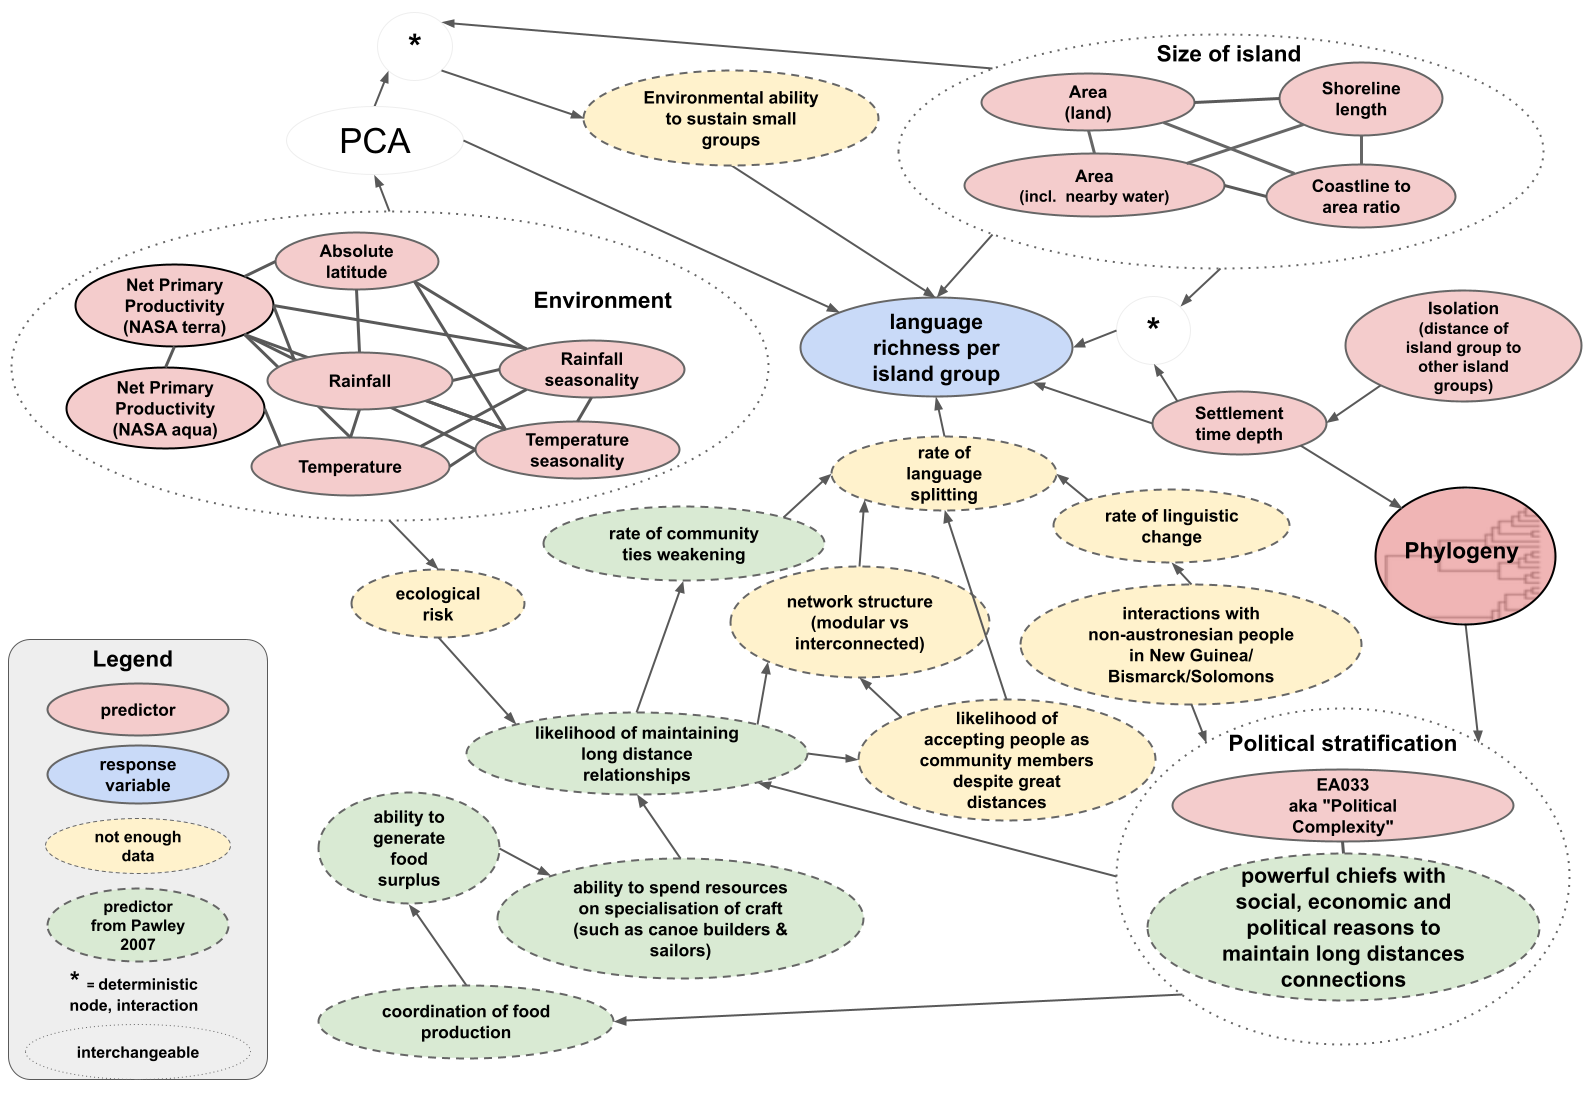
\includegraphics[width=19cm]{Predicting_lgs_DAG_full.png}
\caption{Directed Acyclic Graph of the variables in this study. Blue = variable to be predicted (response).}
\label{Predicting_lgs_DAG_full}
\end{sidewaysfigure}

\newpage
\subsection{Model settings}
\label{appendix_model_settings}
\citep{burkner2017brms}


% BARG
% https://www.nature.com/articles/s41562-021-01177-7/tables/1


%A. Why Bayesian. If the audience requires it, explain what benefits will be gleaned by a Bayesian analysis (as opposed to a frequentist analysis).

%B. Goals of analysis. Explain the goals of the analysis. This prepares the audience for the type of models to expect and how the results will be described.

%Step 1. Explain the model

%A. Data variables. Explain the dependent (predicted) variables and independent (predictor) variables.

%B. Likelihood function and parameters. For every model, explain the likelihood function and all the parameters, distinguishing clearly between parameters of primary theoretical interest and ancillary parameters. If the model is multilevel, be sure that the hierarchical structure is clearly explained, along with any covariance structure if multivariate parameter distributions are used.

%C. Prior distribution. For every model, explain and justify the prior distribution of the parameters in the model.

%D. Formal specification. Include a formal specification (mathematical or computer code) of the likelihood and prior, located either in the main text or in in publicly and persistently accessible online supplementary material.

%E. Prior predictive check. Especially when using informed priors but even with broad priors, it is valuable to report a prior predictive check to demonstrate that the prior really generates simulated data consistent with the assumed prior knowledge.

%Step 2. Report details of the computation

%A. Software. Report the software used, including any specific added packages or plugins.

%B. MCMC chain convergence. Report evidence that the chains have converged, using a convergence statistic such as PSRF, for every parameter or derived value.

%C. MCMC chain resolution. Report evidence that the chains have high resolution, using the ESS, for every parameter or derived value.

%D. If not MCMC. If using some computational procedure other than MCMC, be aware of and report inherently inaccurate approximations, especially for the limits of credible intervals.

%Step 3. Describe the posterior distribution

%A. Posterior predictive check. Provide a posterior predictive check to show that the model usefully mimics the data.

%B. Summarize posterior of variables. For continuous parameters, derived variables and predicted values, report the central tendency and limits of the credible interval. Explicitly state whether you are using density-based values (mode and HDI) or quantile-based values (median and ETI), and state the mass of the credible interval (for example, 95%).

%C. BF and posterior model probabilities. If conducting model comparison or hypothesis testing, report the BF and posterior probabilities of models for a range of prior model probabilities.

%Step 4. Report decisions (if any) and their criteria

%A. Why decisions? Explain why the decisions are theoretically meaningful and which decision procedure is being used. Regardless of which decision procedure is used, if it addresses null values, it should be able to accept the null value not only reject it.

%B. Loss function. If utilities and a loss function for a decision rule are defined, these should be explained and reported.

%C. ROPE limits. If using a continuous-parameter posterior distribution as the basis for decision, state and justify the limits of the ROPE and the required probability mass.

%D. BF, decision threshold and model probabilities. If using model comparison or hypothesis testing as the basis for a decision, state and justify the decision threshold for the posterior model probability, and the minimum prior model probability that would make the posterior model probability exceed the decision threshold.

%E. Estimated values too. If deciding about null values, always also report the estimate of the parameter value (central tendency and credible interval).

%Step 5. Report sensitivity analysis

%A. For broad priors. If the prior is intended to be vague or only mildly informed so that it has minimal influence on the posterior, show that other vague priors produce similar posterior results.

%B. For informed priors. If the prior is informed by previous research, show what posterior results from a vague prior or from a range of differently informed priors.

%C. For default priors. If using a default prior, show the effect of varying its settings. Be sure that the range of default priors constitutes theoretically meaningful priors, and consider whether they mimic plausible empirically informed priors.

%D. BFs and model probabilites. If the analysis involves model comparison or hypothesis testing, then for each prior report not only the BFs but also the posterior model probabilities for a range of prior model probabilities.

%E. Decisions. If making decisions, report whether decisions change under different priors. For BFs, report changes in the minimum prior model probability needed to achieve decisive posterior model probability.

\newpage
\subsection{BRMS model tables}
\label{BRMS_model_tables}
Following the principles of Bayesian Analysis Reporting Guidelines \citep{kruschke2021bayesian}, we are reporting Rhat (convergence of chains) and ESS

\begin{landscape}
% latex table generated in R 4.3.1 by xtable 1.8-4 package
% Thu Aug 24 21:33:07 2023
\begin{table}[ht]
\centering
\begin{tabular}{p{5cm}p{2cm}p{2cm}p{2cm}p{2cm}p{2cm}p{2cm}p{2cm}}
  \toprule
term & Estimate & Est.Error & l-95\% CI & u-95\% CI & Does 95\% interval straddle zero? & Bulk ESS & Tail ESS \\ 
  \midrule
EA033 & -0.848 & 0.119 & -1.089 & -0.621 & no & 86903.116 & 78680.772 \\ 
  environ\_PC1 & -0.339 & 0.184 & -0.700 & 0.022 & yes & 62722.893 & 72819.676 \\ 
  environ\_PC1:Shoreline & 0.173 & 0.142 & -0.096 & 0.460 & yes & 56177.329 & 72113.543 \\ 
  environ\_PC2 & 0.191 & 0.199 & -0.202 & 0.577 & yes & 55715.732 & 68364.257 \\ 
  environ\_PC3 & 0.166 & 0.144 & -0.117 & 0.448 & yes & 77362.236 & 78385.290 \\ 
  Intercept & 0.260 & 0.168 & -0.080 & 0.583 & yes & 69183.952 & 73793.051 \\ 
  Time depth & 0.482 & 0.136 & 0.224 & 0.758 & yes & 85944.050 & 77272.546 \\ 
  Shoreline & 0.640 & 0.175 & 0.300 & 0.992 & yes & 57283.173 & 69766.242 \\ 
  Shoreline:environ\_PC2 & -0.343 & 0.190 & -0.700 & 0.048 & yes & 60024.526 & 67019.249 \\ 
  Shoreline:environ\_PC3 & 0.097 & 0.124 & -0.158 & 0.330 & yes & 75070.000 & 75363.372 \\ 
  Shoreline:Time depth & 0.452 & 0.128 & 0.210 & 0.714 & yes & 90331.190 & 73841.991 \\ 
   \bottomrule
\end{tabular}
\caption{Table of BRMS model outcomes, shared-language island groups (all observations included).} 
\label{BRMS_effects_medium}
\end{table}

\end{landscape}

\begin{landscape}
% latex table generated in R 4.3.1 by xtable 1.8-4 package
% Thu Aug 24 00:32:11 2023
\begin{table}[ht]
\centering
\begin{tabular}{p{5cm}p{2cm}p{2cm}p{2cm}p{2cm}p{2cm}p{2cm}p{2cm}}
  \toprule
term & Estimate & Est.Error & l-95\% CI & u-95\% CI & Does 95\% interval straddle zero? & Bulk ESS & Tail ESS \\ 
  \midrule
EA033 & -0.918 & 0.063 & -1.044 & -0.797 & no & 86638.570 & 78681.590 \\ 
  environ\_PC1 & 0.036 & 0.136 & -0.227 & 0.306 & yes & 97731.893 & 78917.307 \\ 
  environ\_PC1:Shoreline & 0.147 & 0.105 & -0.056 & 0.355 & yes & 73831.690 & 79033.044 \\ 
  environ\_PC2 & -0.696 & 0.150 & -0.988 & -0.399 & no & 80961.192 & 79018.840 \\ 
  Intercept & -0.227 & 0.157 & -0.546 & 0.070 & yes & 89617.251 & 81197.703 \\ 
  Time depth & 0.407 & 0.154 & 0.104 & 0.709 & yes & 72478.466 & 75930.439 \\ 
  Shoreline & 1.008 & 0.166 & 0.681 & 1.332 & yes & 78008.053 & 75478.131 \\ 
  Shoreline:environ\_PC2 & 0.084 & 0.133 & -0.187 & 0.336 & yes & 65445.484 & 75126.246 \\ 
  Shoreline:Time depth & 0.823 & 0.133 & 0.570 & 1.090 & yes & 63779.842 & 72874.694 \\ 
   \bottomrule
\end{tabular}
\caption{Table of BRMS model outcomes, overnight-distance island groups (all observations included).} 
\label{BRMS_effects_SBZR}
\end{table}

\end{landscape}



\newpage
\subsection{Supplementary figures}
\label{appendix_supp_figs}

\begin{figure}[ht]

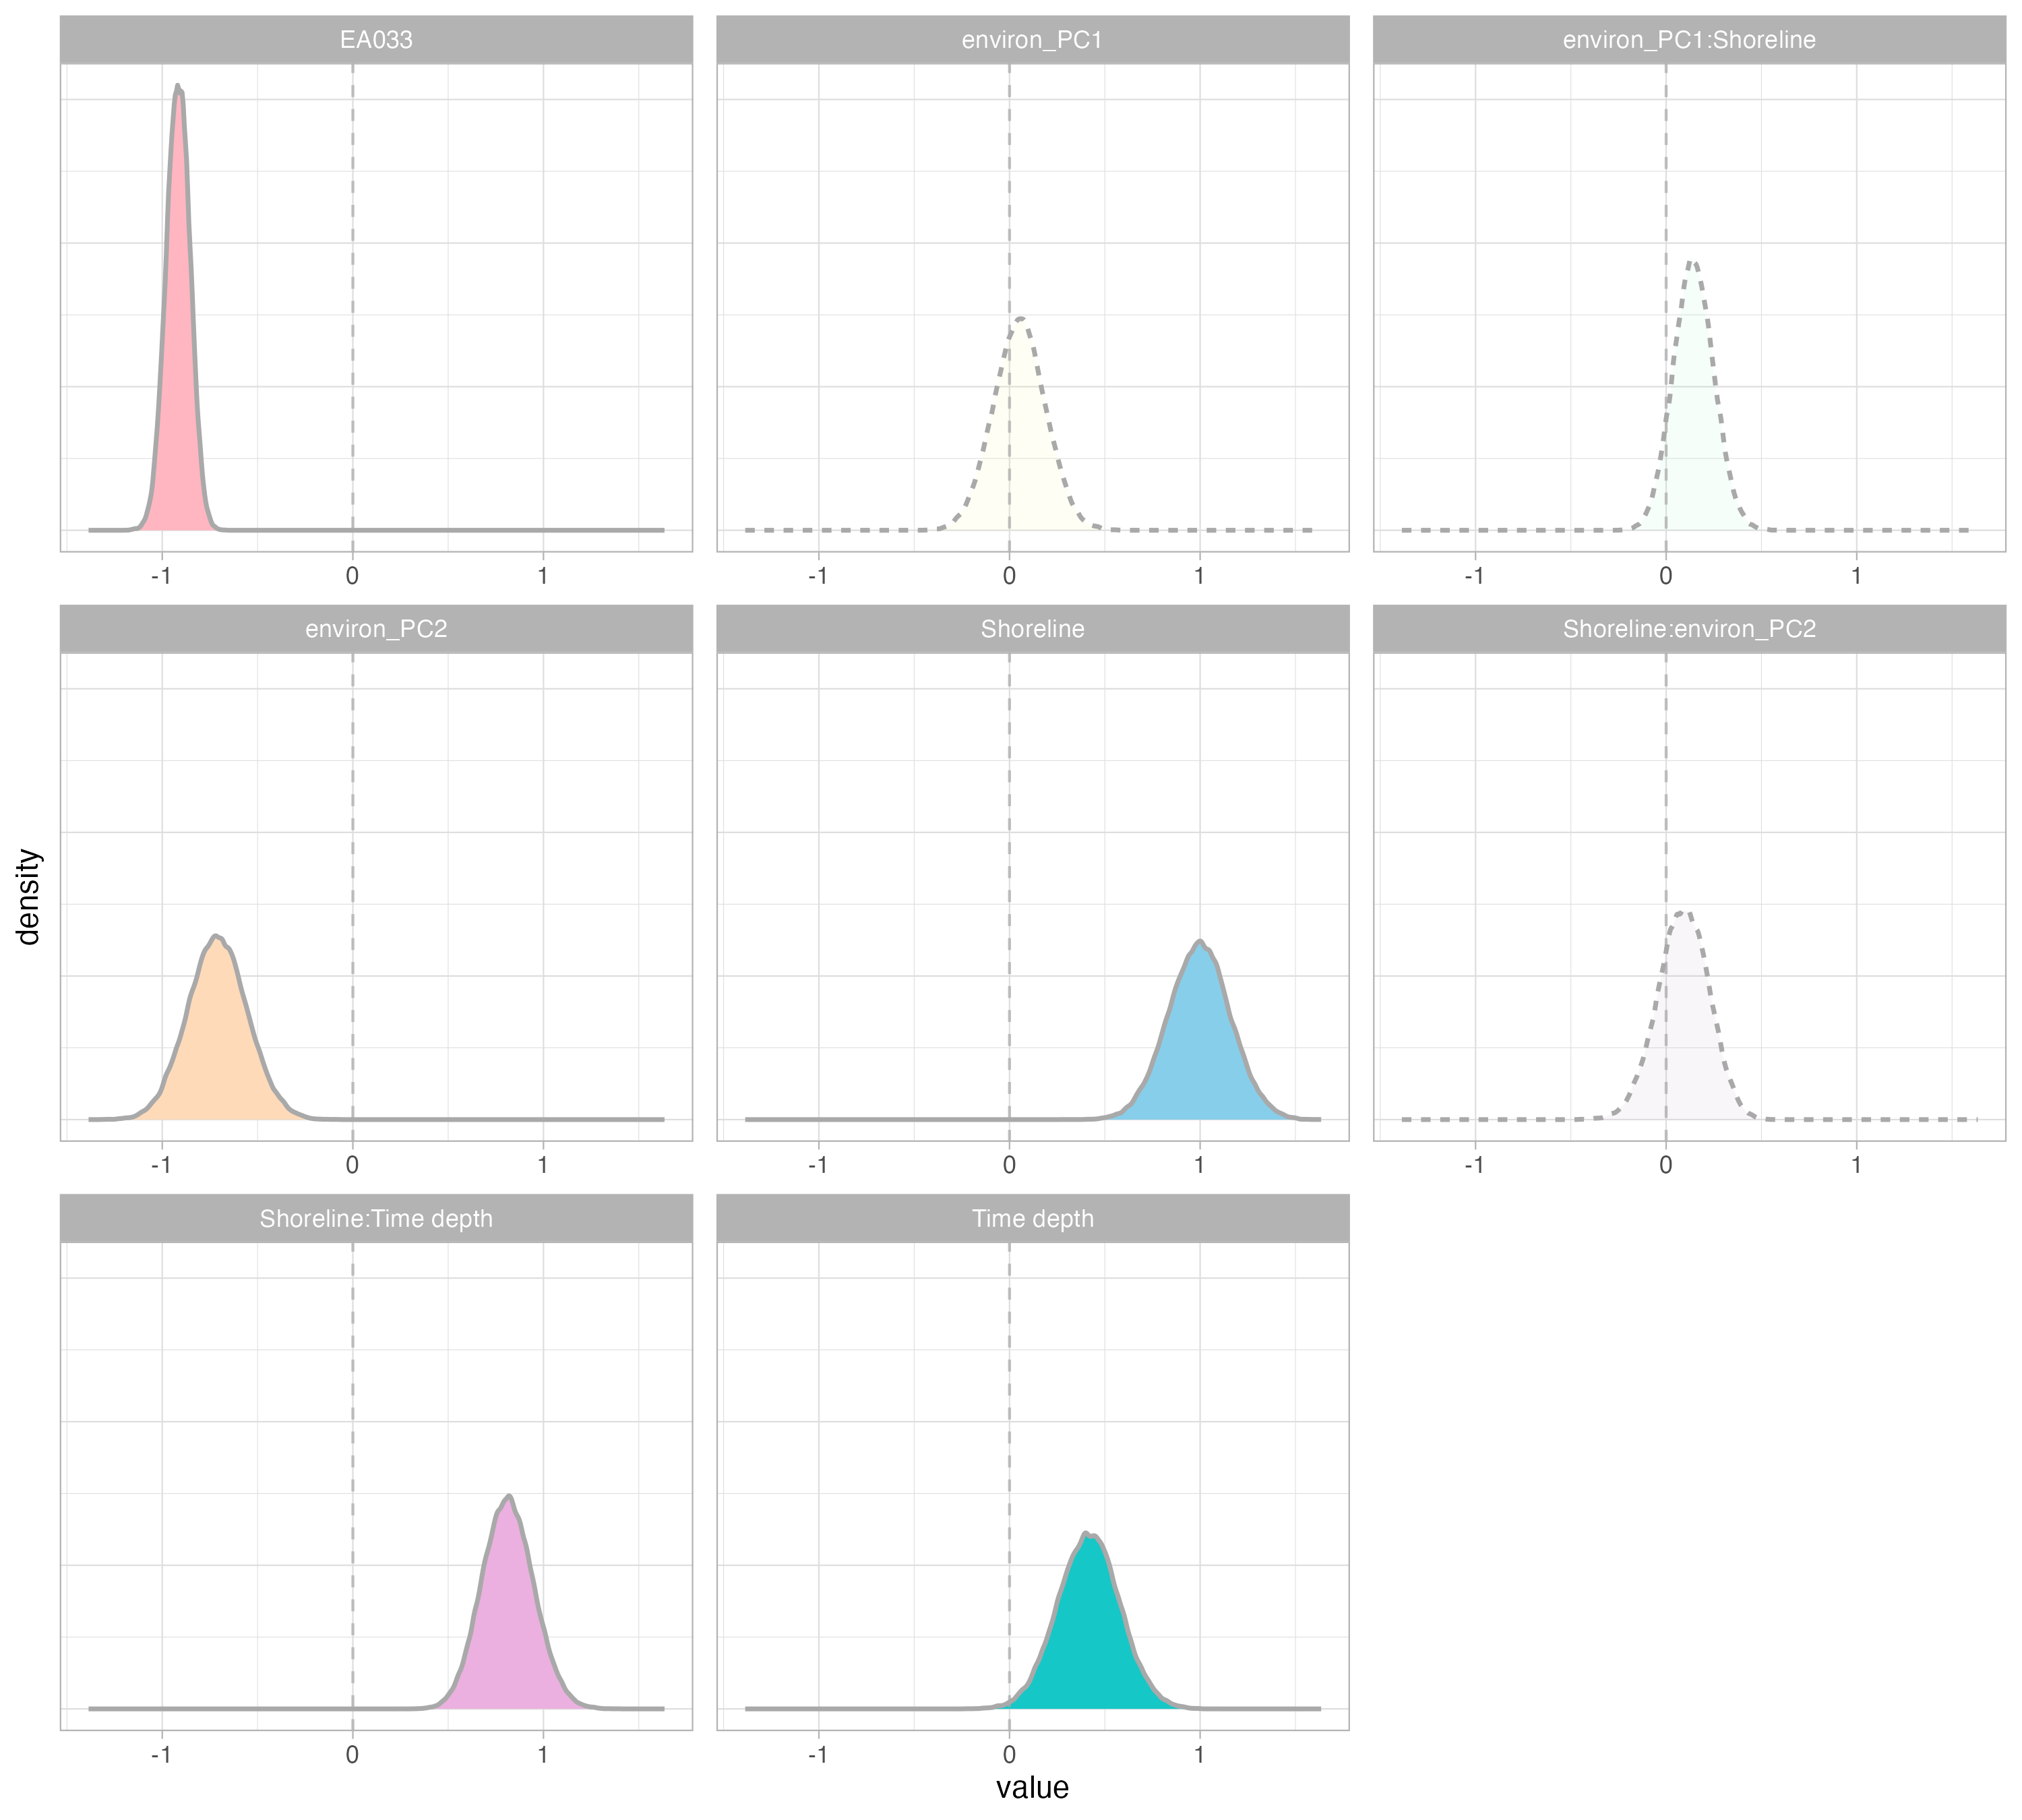
\includegraphics[width=15cm]{brms_SBZR_group_full_effect_ridge_panels_plot.png}
\caption{Coefficient distribution of BRMS model, using overnight sailing distances island groups with all observations.}
\label{brms_SBZR_group_full_effect_ridge_panels}
\end{figure}

\begin{figure}[ht]
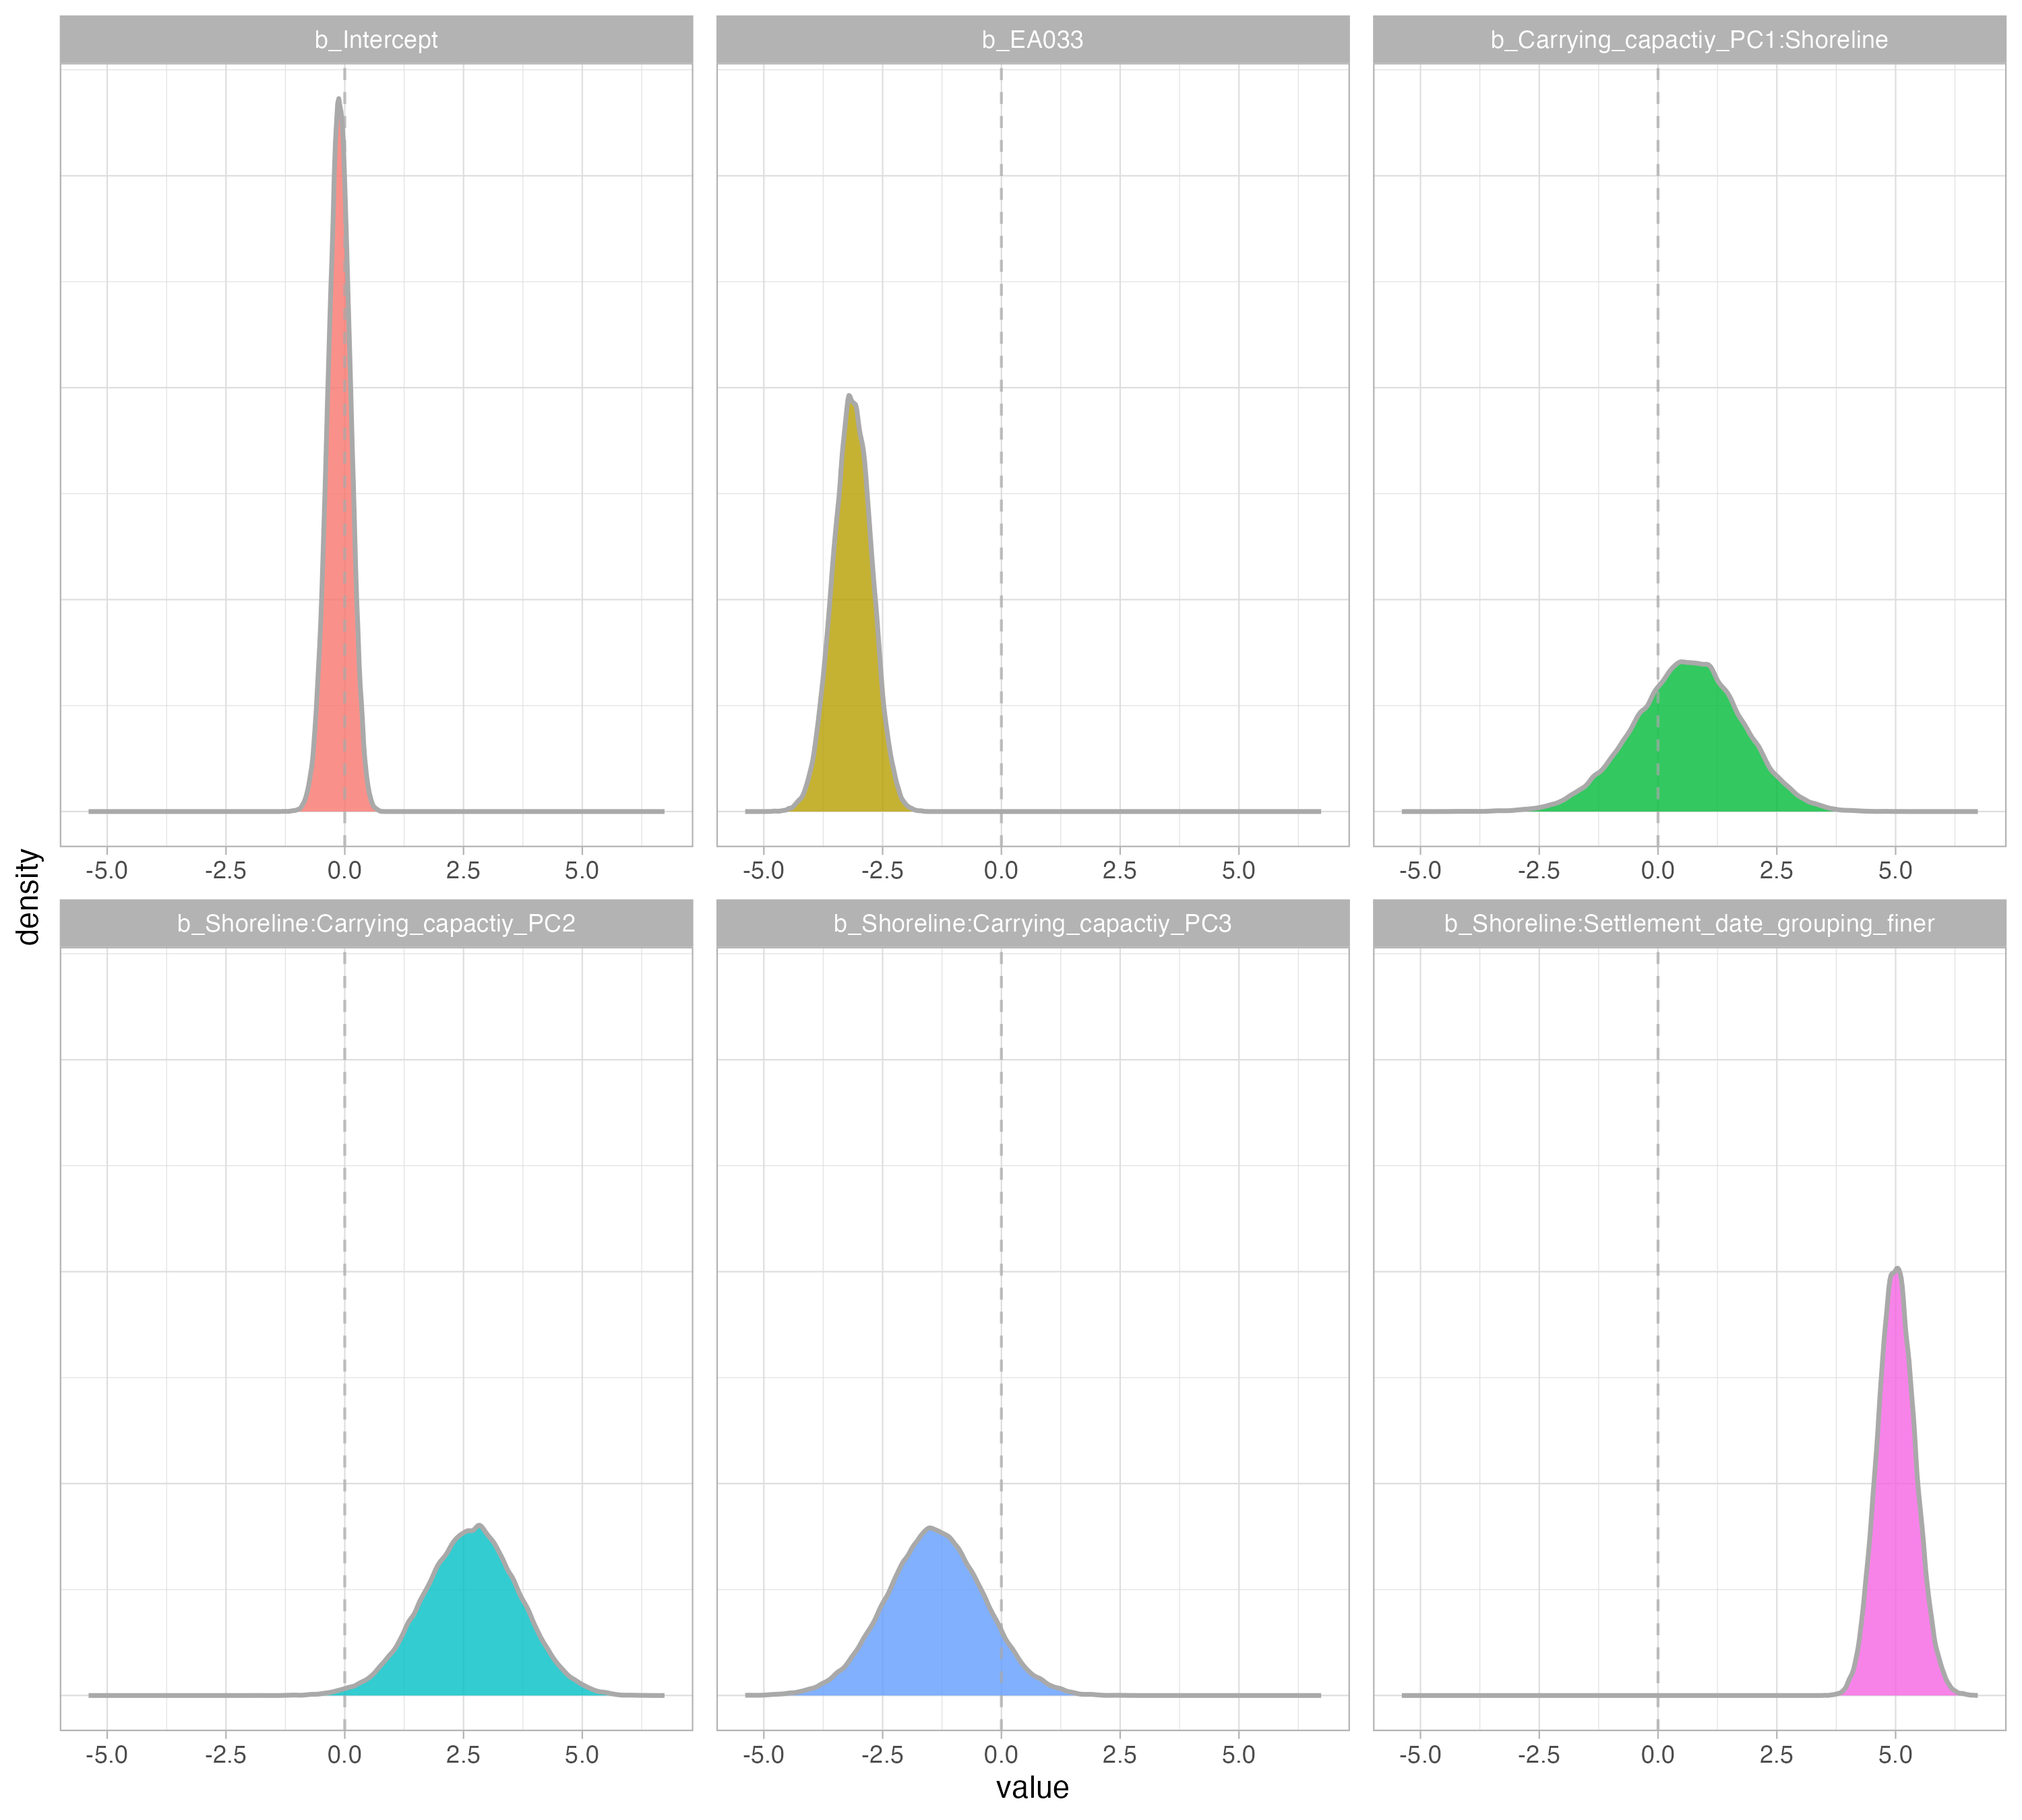
\includegraphics[width=15cm]{brms_medium_group_full_effect_ridge_panels_plot.png}
\caption{Coefficient distribution of BRMS model, using shared-language island groups with all observations.}
\label{brms_medium_group_full_effect_ridge_panels}
\end{figure}

\begin{figure}[ht]
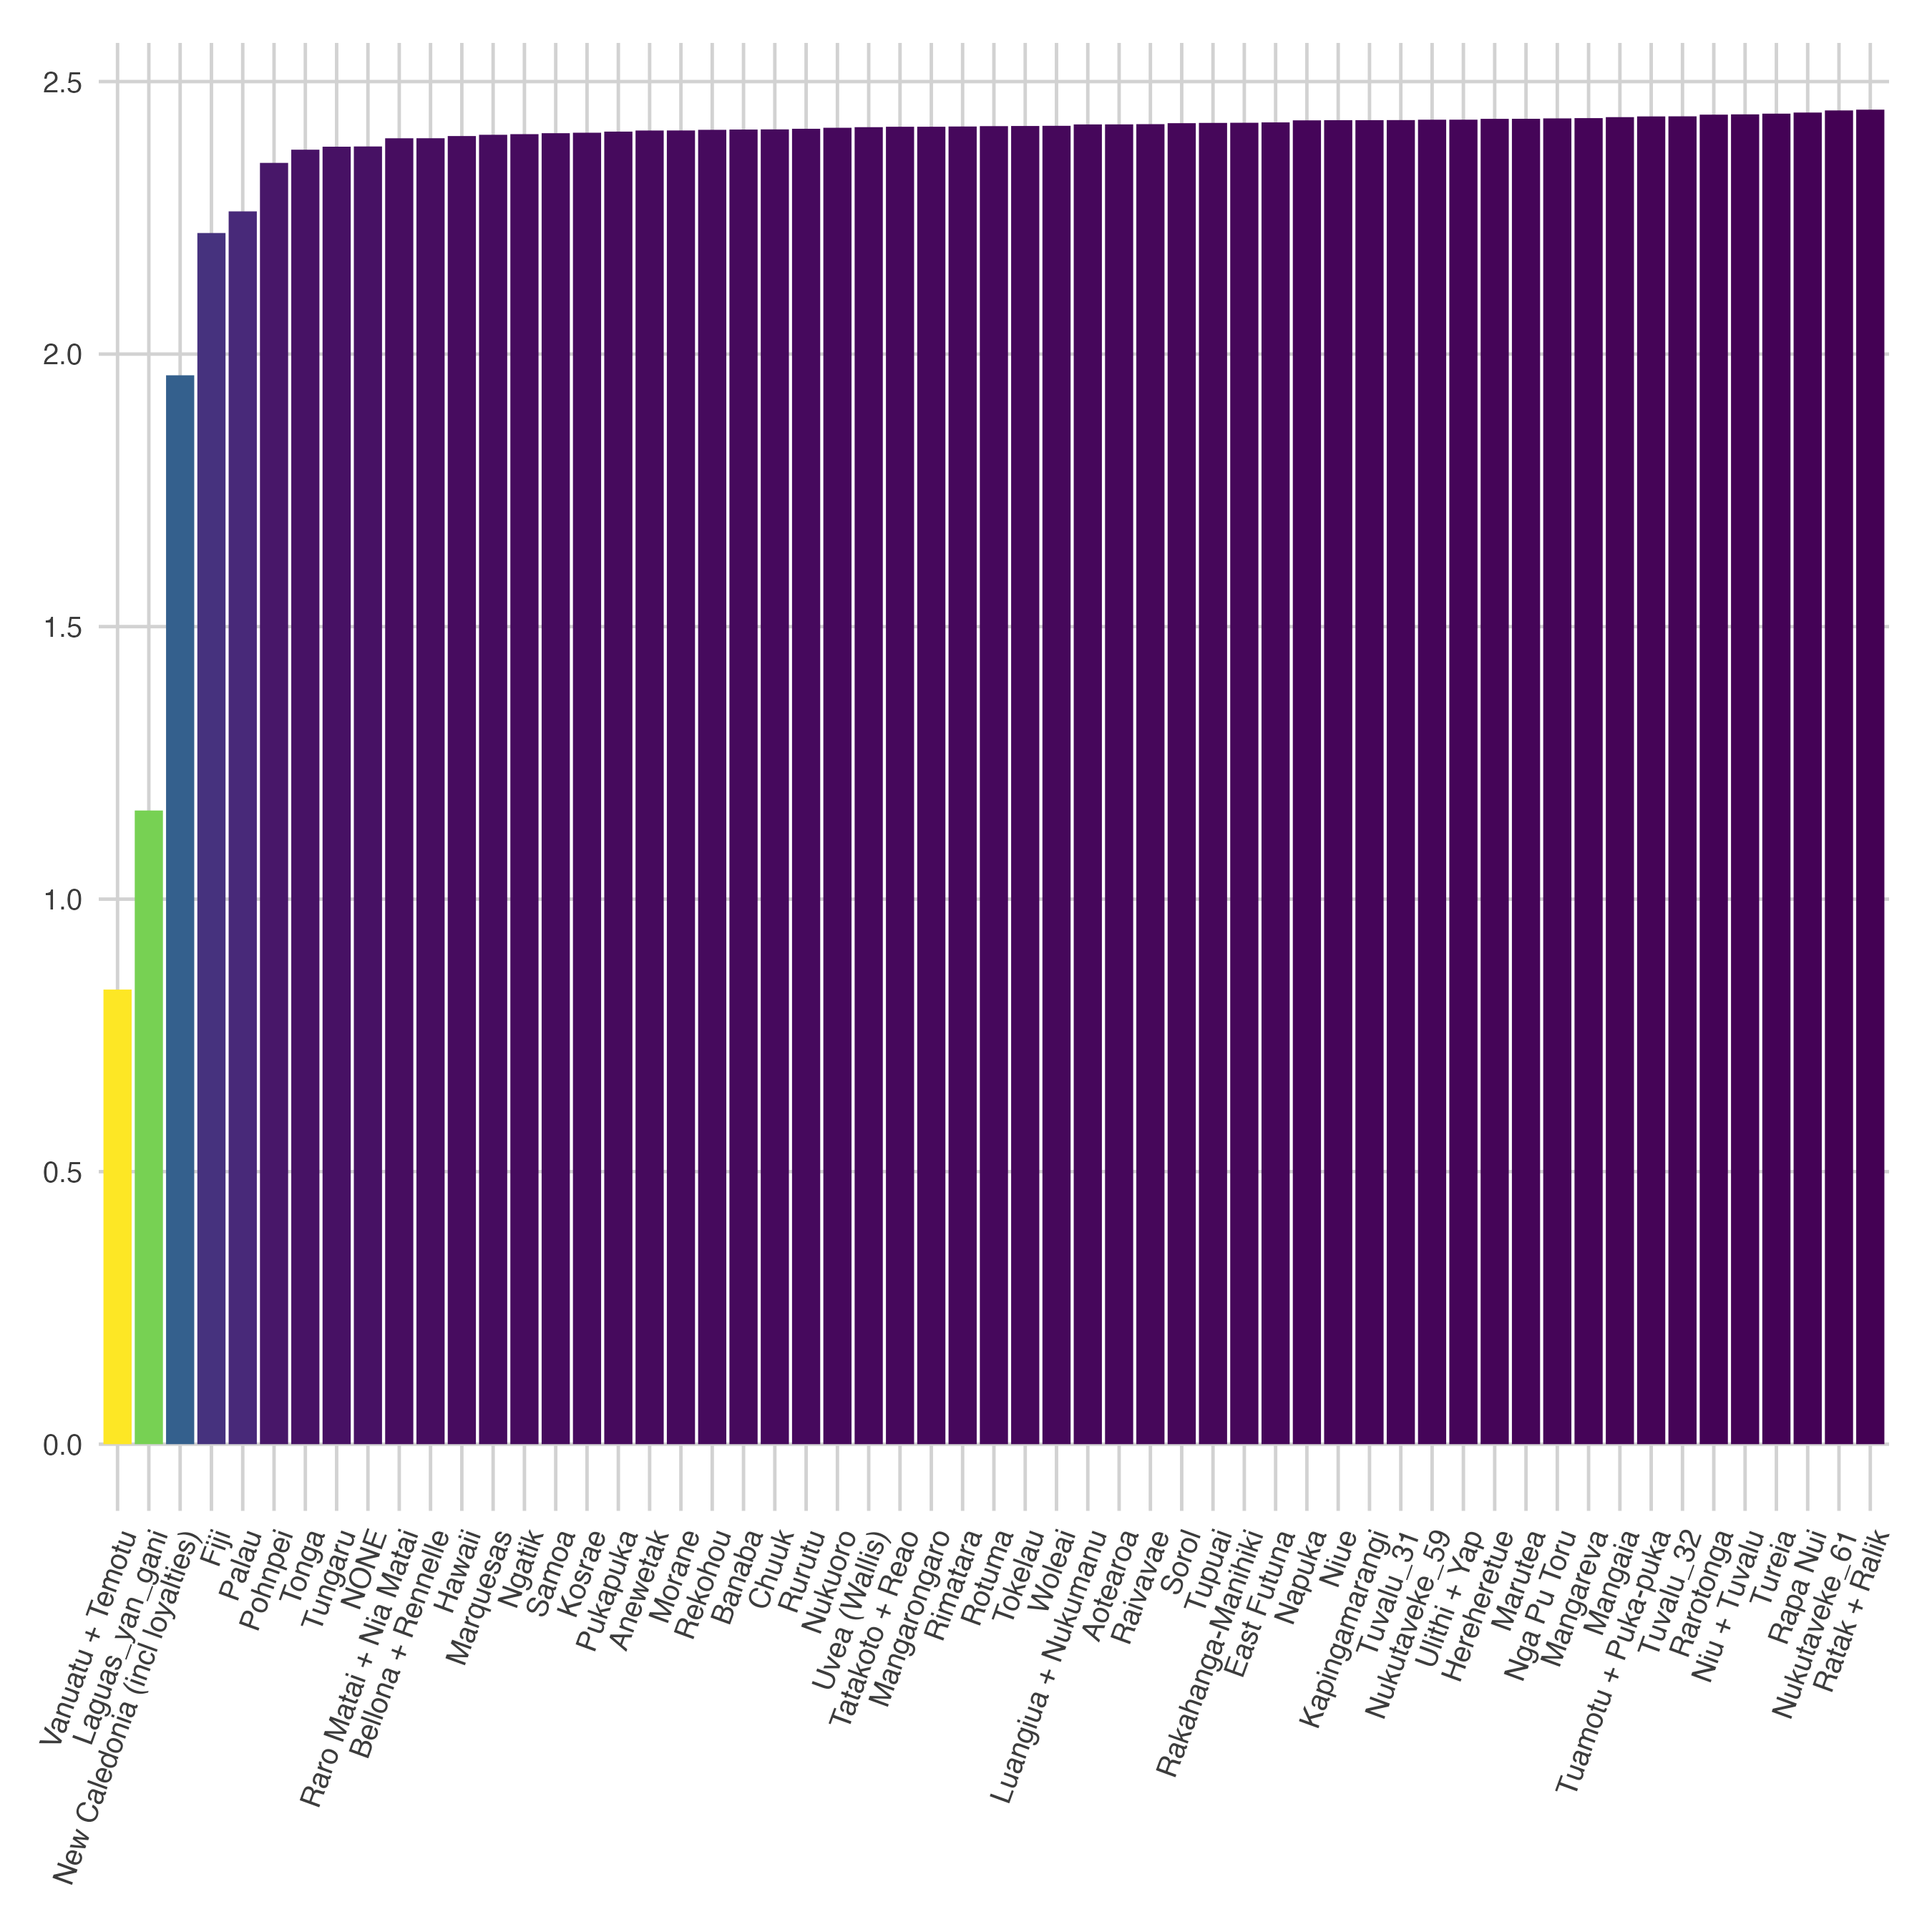
\includegraphics[width=15cm]{brms_SBZR_dropped_out_plot_diff.png}
\caption{Mean absolute difference of predicted and observed number of languages per island group (overnight sailing distances group). Every column represents a new run of the model with a particular group dropped out from the observations. When Vanuatu + Temotu is dropped out, the model predicts numbers that are more similar to the observed values than when that island group is included in the model.}
\label{brms_SBZR_dropped_out_plot_diff}
\end{figure}

\begin{figure}[ht]
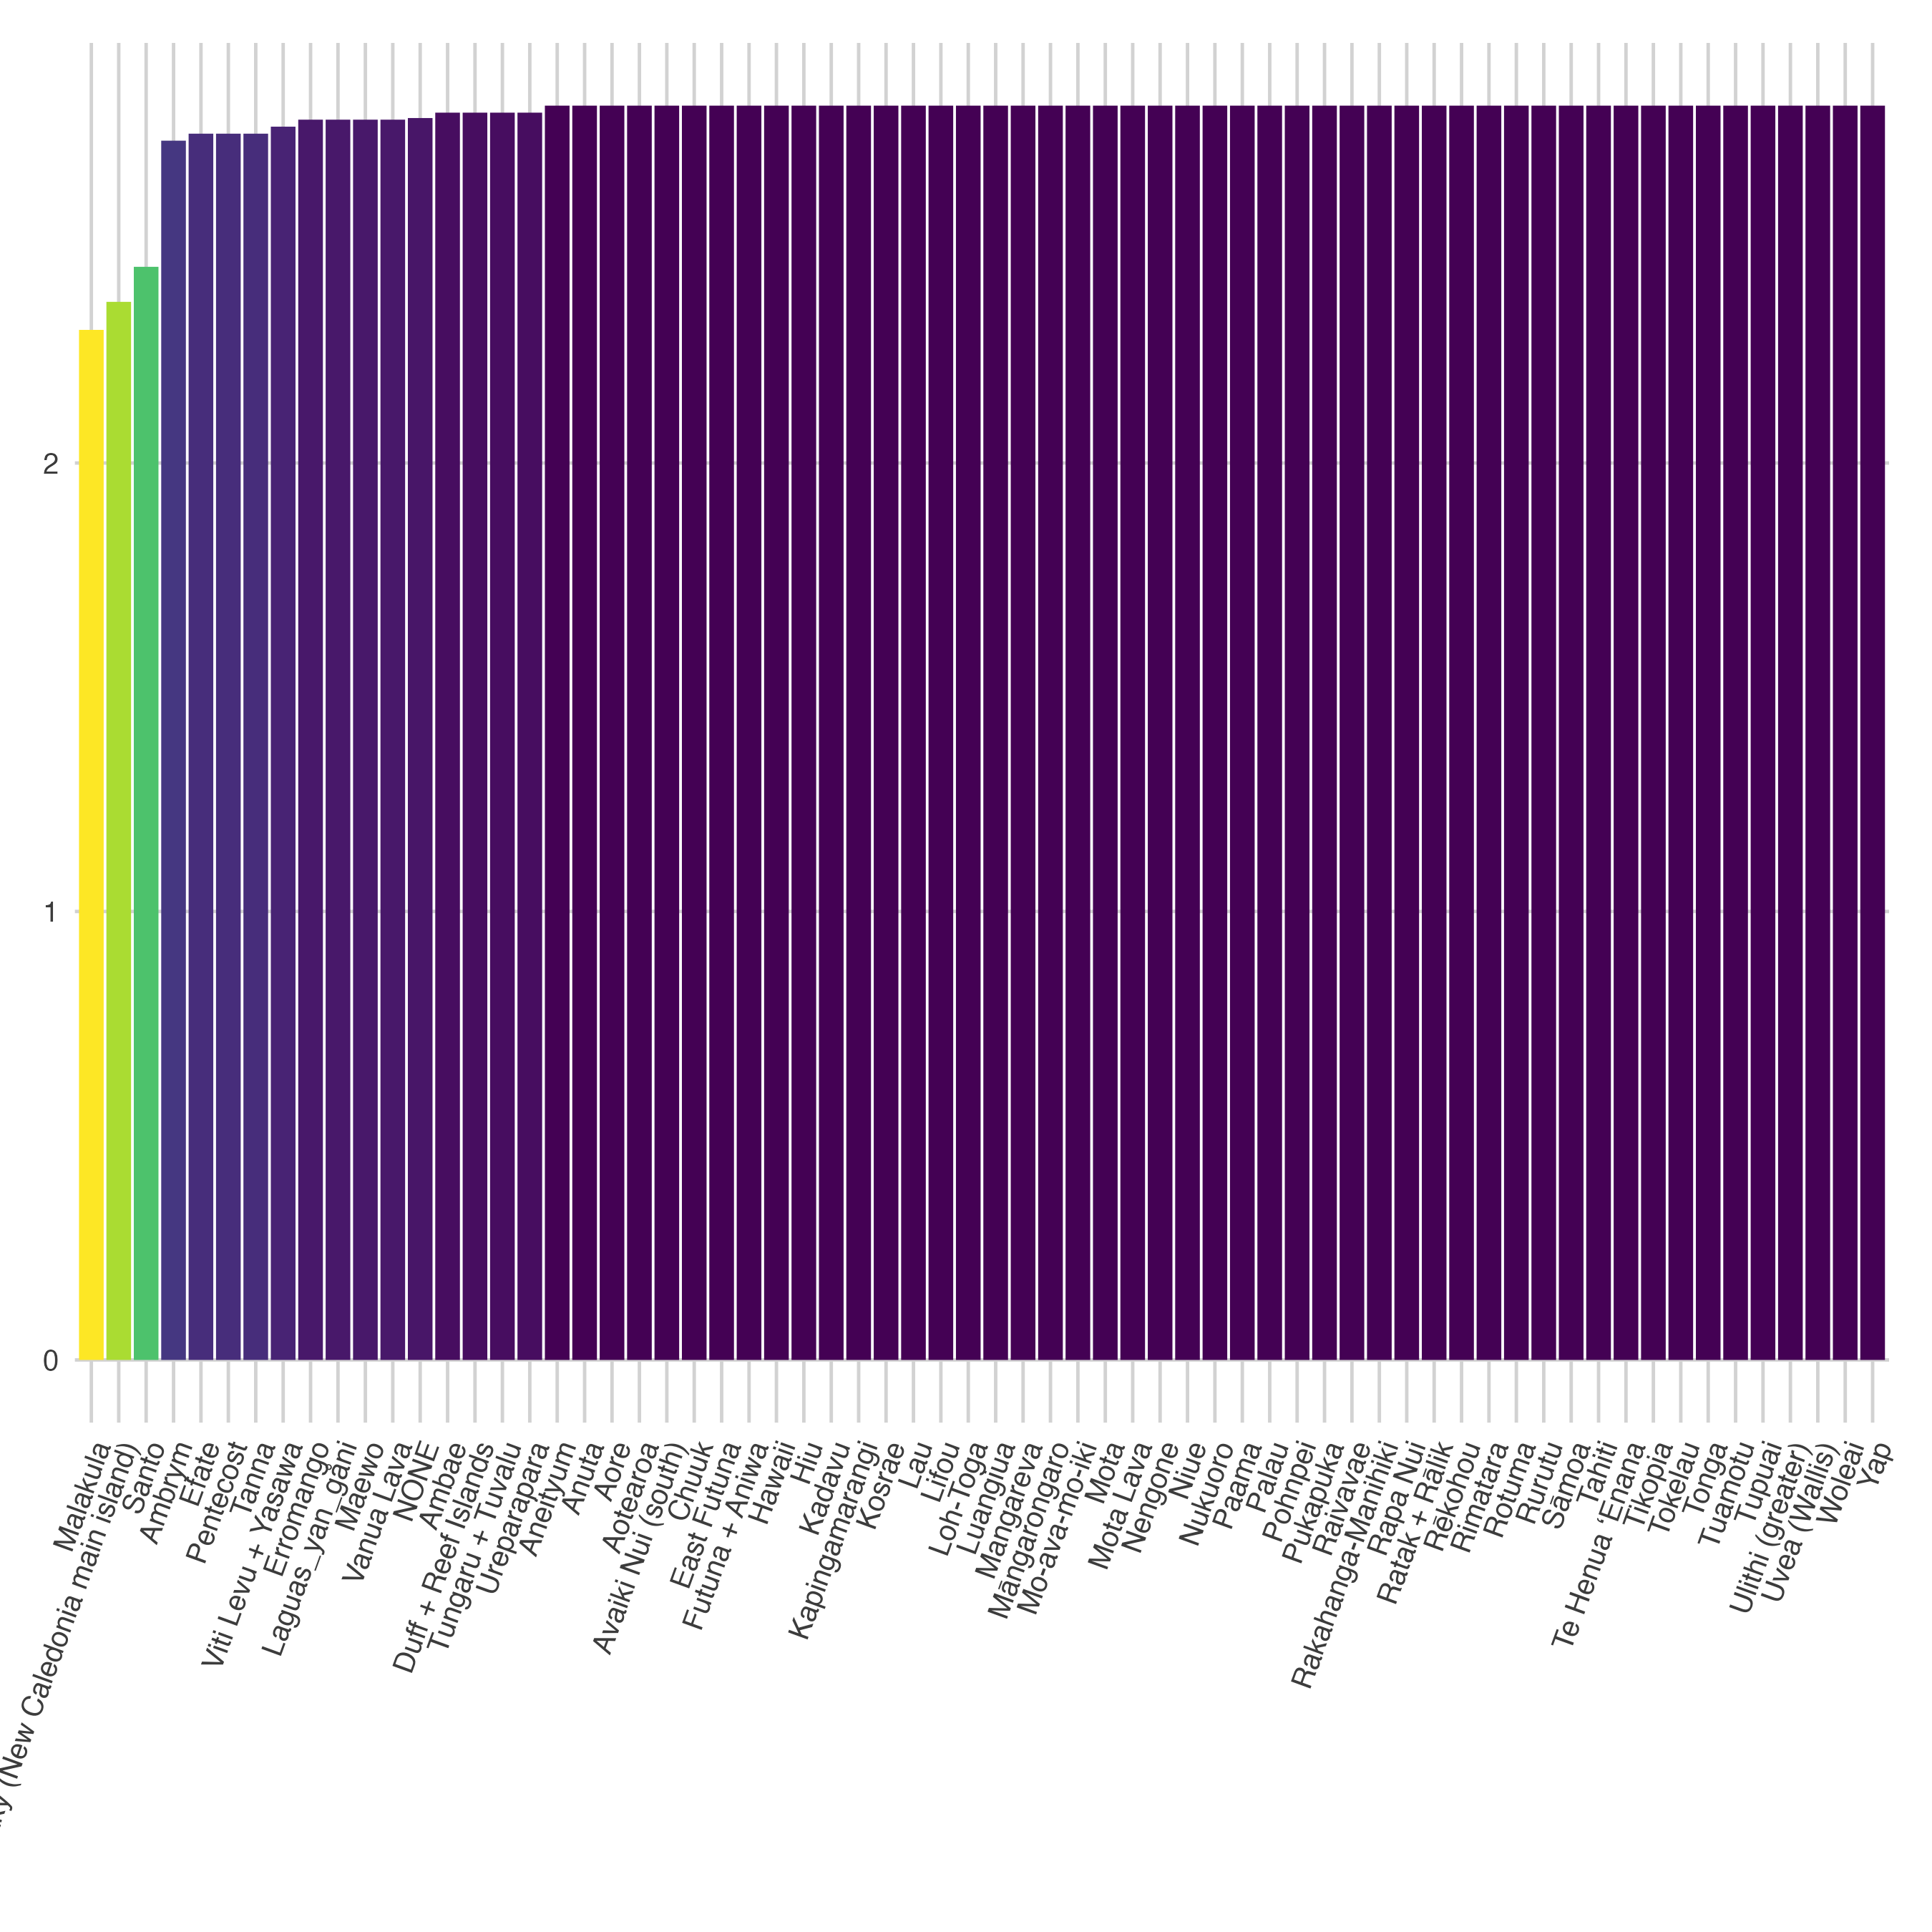
\includegraphics[width=15cm]{brms_medium_dropped_out_plot_diff.png}
\caption{Mean absolute difference of predicted and observed number of languages per island group (shared language grouping). Every column represents a new run of the model with a particular group dropped out from the observations. When Malakula is dropped out, the model predicts numbers that are more similar to the observed values than when that island group is included in the model.}
\label{brms_medium_dropped_out_plot_diff}
\end{figure}


\begin{figure}[ht]
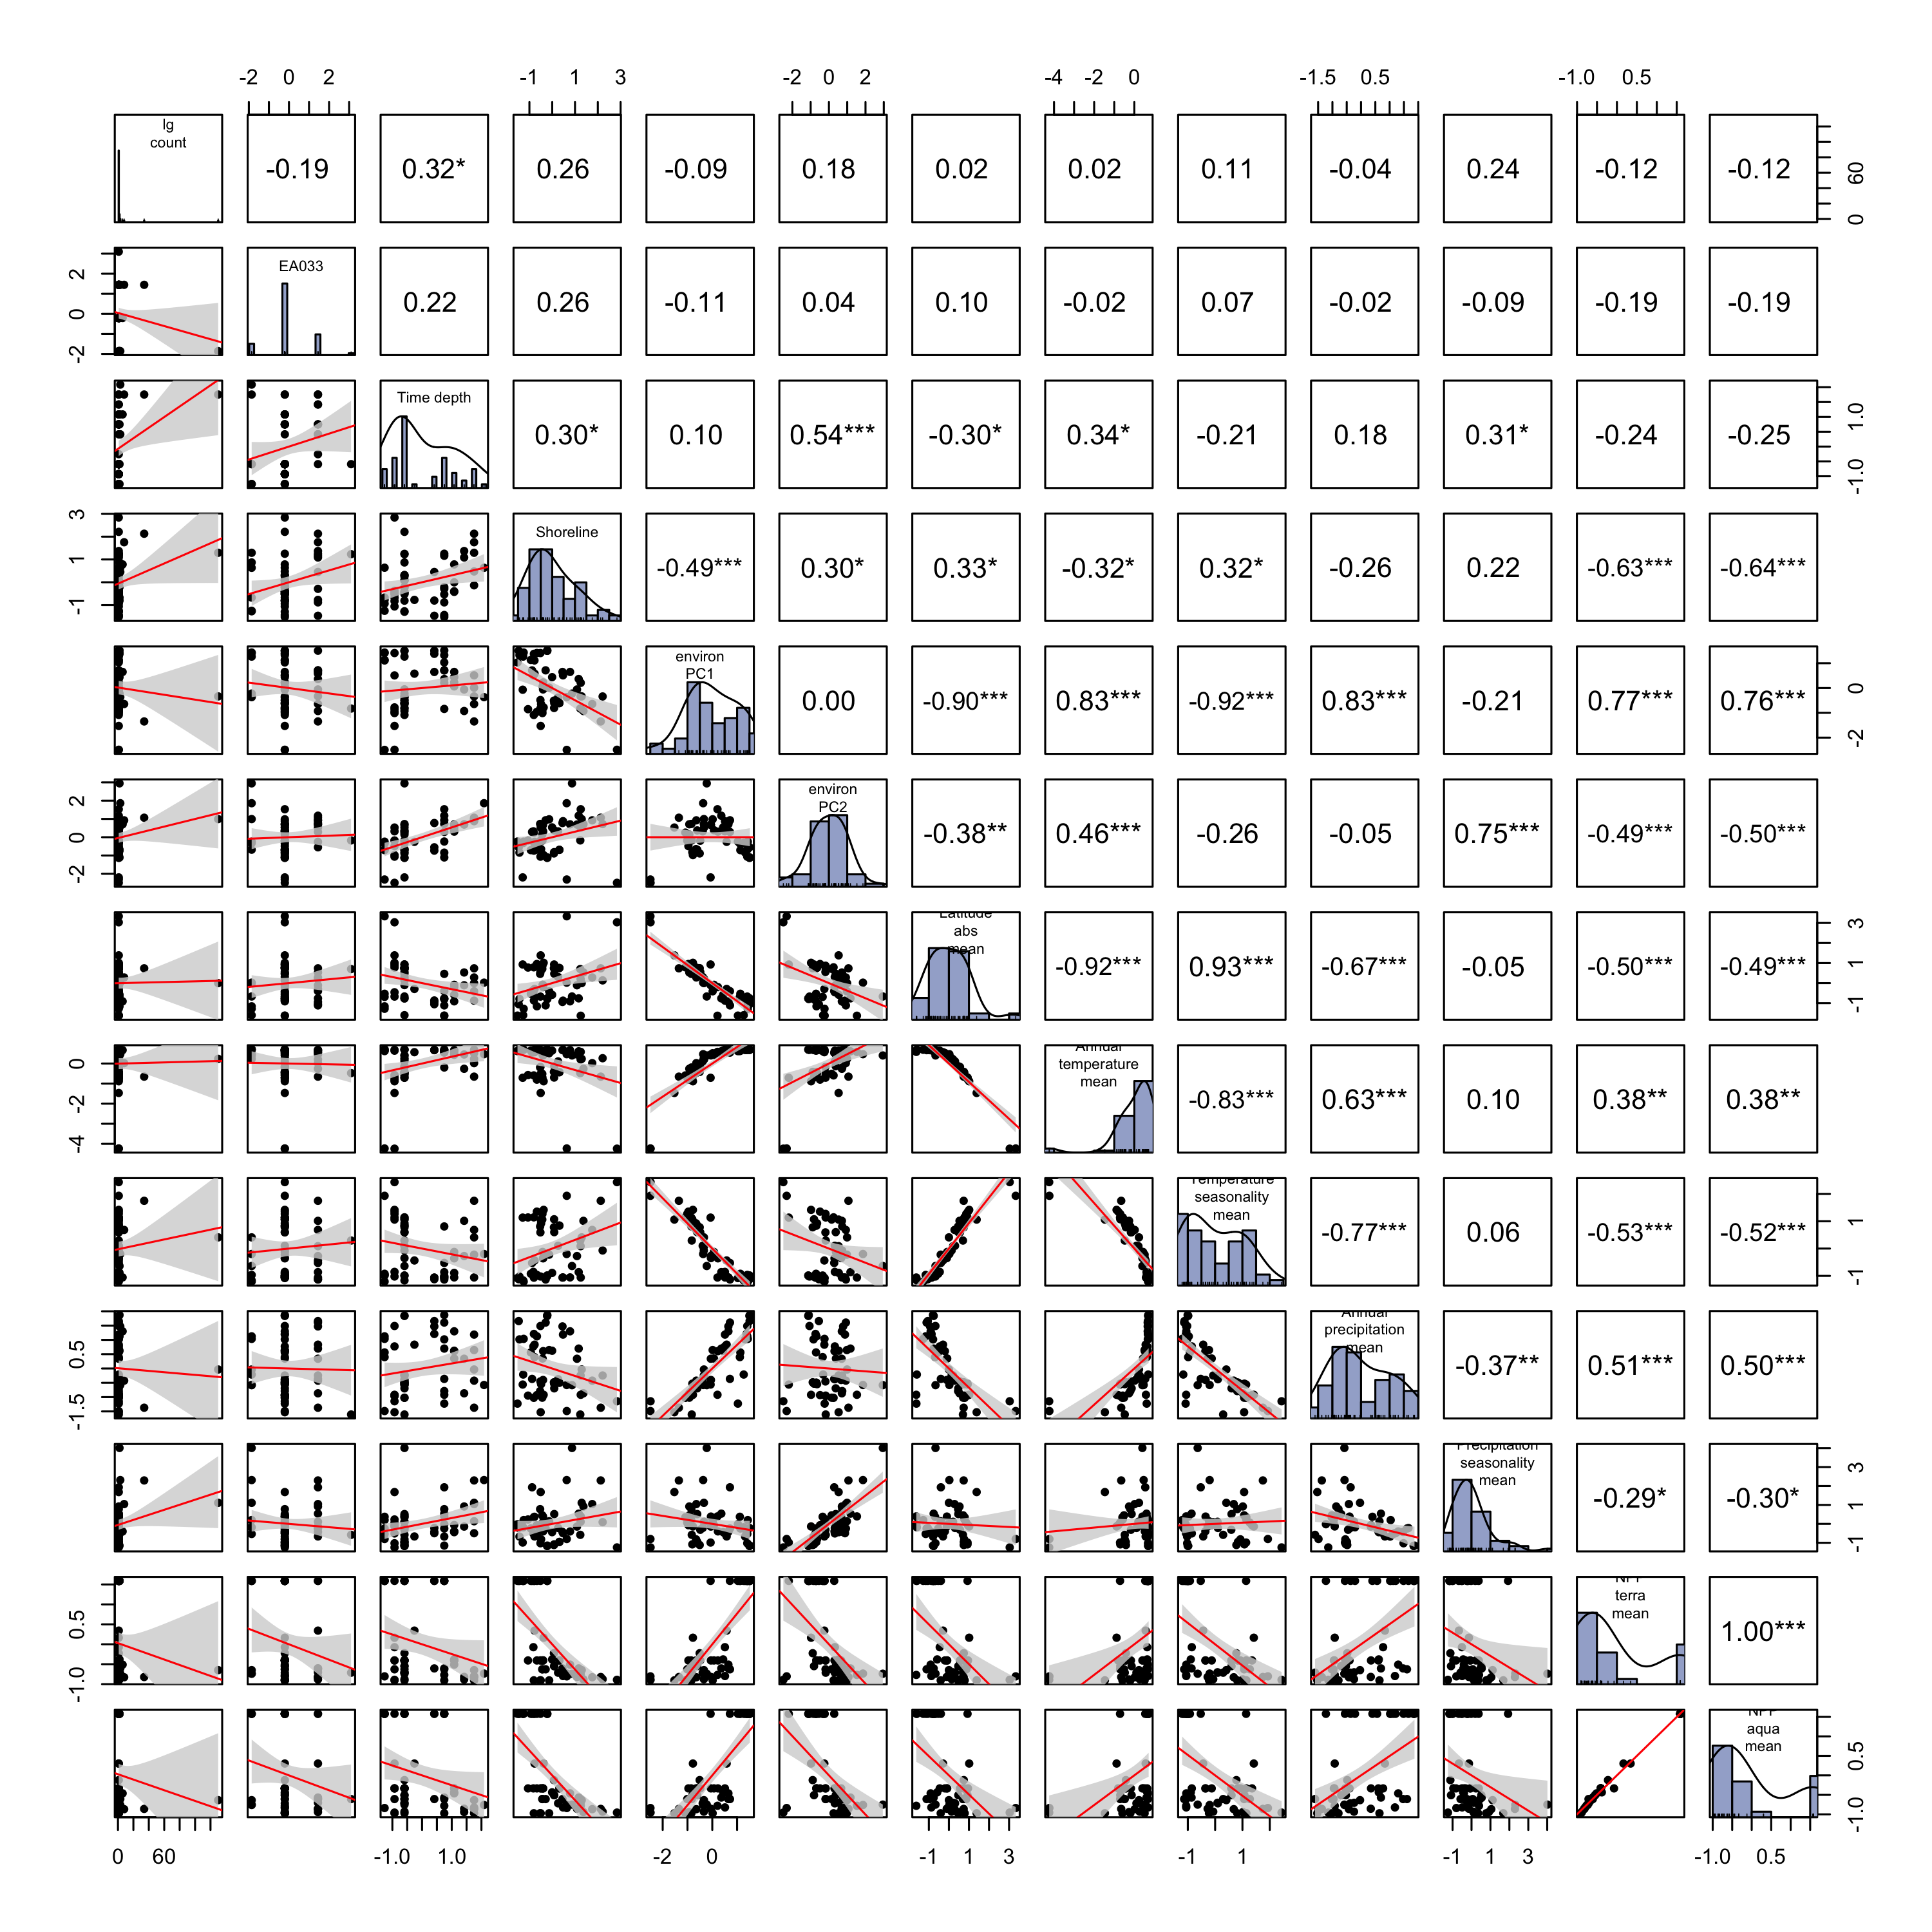
\includegraphics[width=15cm]{latex/SPLOM_SBZR_all_variables.png}
\caption{Scatterplot matrix of all variables available, over overnight-sailing-groups.}
\label{SPLOM_SBZR_all_variables}
\end{figure}

\begin{figure}[ht]
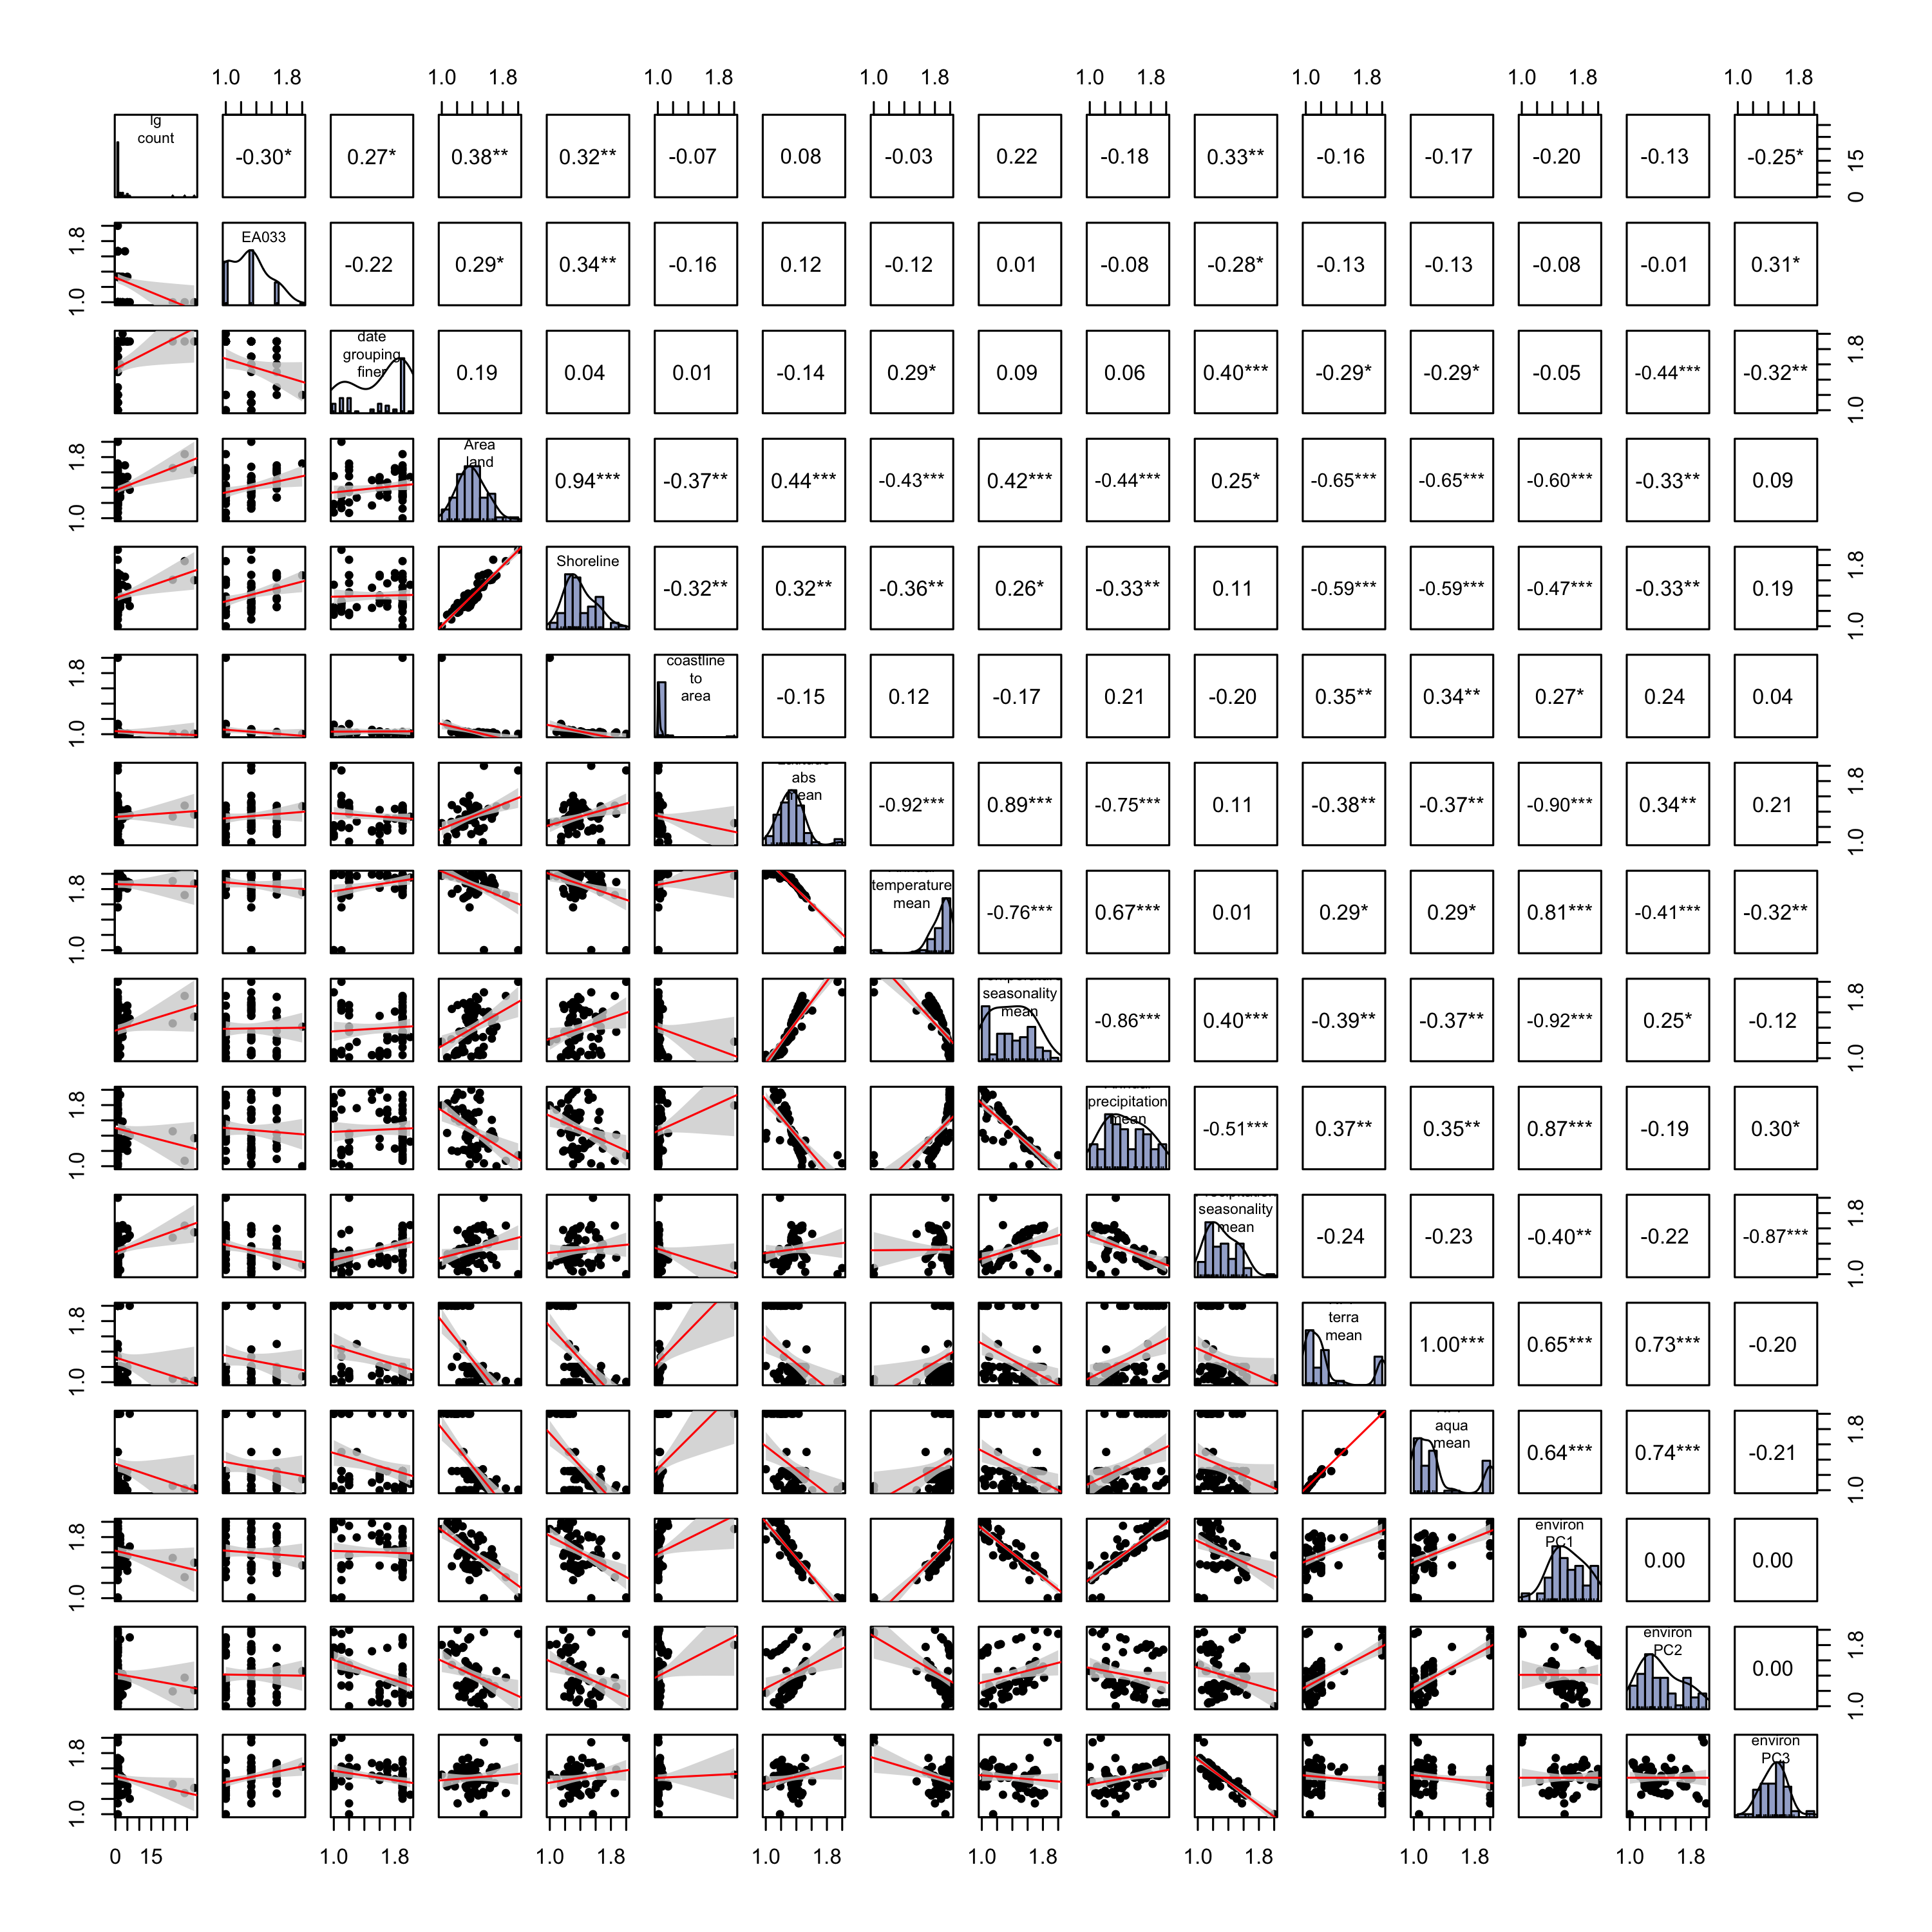
\includegraphics[width=15cm]{latex/SPLOM_medium_all_variables.png}
\caption{Scatterplot matrix of all variables available, over shared-language-groups.}
\label{SPLOM_medium_all_variables}
\end{figure}



\FloatBarrier
\newpage
\subsection{R-packages used}
\label{appendix_r_packages}

All the analysis for this research project was done in the free and open source programming language R, using a multitude of packages. All code and data for this project are available in the locations listed in Supplementary material section \ref{supp_data_availability}. The scripts have been written so that any user of R can execute them. Please see the bibliography for information on package versions. Below are citations for all used packages.

\input{latex/citation_keys.txt}.

\end{document}
